\documentclass[a4paper,UKenglish,cleveref, autoref, thm-restate,anonymous]{lipics-v2021}
%This is a template for producing LIPIcs articles. 
%for A4 paper format use option "a4paper", for US-letter use option "letterpaper"
%for british hyphenation rules use option "UKenglish", for american hyphenation rules use option "USenglish"
%for section-numbered lemmas etc., use "numberwithinsect"
%for enabling cleveref support, use "cleveref"
%for enabling autoref support, use "autoref"
%for anonymousing the authors (e.g. for double-blind review), add "anonymous"
%for enabling thm-restate support, use "thm-restate"
%for producing a PDF according the PDF/A standard, add "pdfa"

%\pdfoutput=1 %uncomment to ensure pdflatex processing (mandatatory e.g. to submit to arXiv)
%\hideLIPIcs  %uncomment to remove references to LIPIcs series (logo, DOI, ...), e.g. when preparing a pre-final version to be uploaded to arXiv or another public repository

%\graphicspath{{./graphics/}}%helpful if your graphic files are in another directory

\usepackage{panbench}

\title{\panbench: A Comparative Benchmarking Tool for Dependently-Typed Languages}

\author{Reed Mullanix}{Department of Computing and Software, McMaster University, Canada}{mullanir@mcmaster.ca}{https://orcid.org/0000-0002-7970-4961}{}
\author{Jacques Carette}{Department of Computing and Software, McMaster University, Canada}{carette@mcmaster.ca}{https://orcid.org/0000-0001-8993-9804}{}

\authorrunning{R. Mullanix and J. Carette}

\Copyright{Reed Mullanix and Jacques Carette}

\ccsdesc[100]{\textcolor{red}{Replace ccsdesc macro with valid one}} %TODO mandatory: Please choose ACM 2012 classifications from https://dl.acm.org/ccs/ccs_flat.cfm 

\keywords{\textcolor{red}{Benchmarking, dependent types, testing}}

\category{} %optional, e.g. invited paper

\relatedversion{} %optional, e.g. full version hosted on arXiv, HAL, or other respository/website
%\relatedversiondetails[linktext={opt. text shown instead of the URL}, cite=DBLP:books/mk/GrayR93]{Classification (e.g. Full Version, Extended Version, Previous Version}{URL to related version} %linktext and cite are optional

%\supplement{}%optional, e.g. related research data, source code, ... hosted on a repository like zenodo, figshare, GitHub, ...
%\supplementdetails[linktext={opt. text shown instead of the URL}, cite=DBLP:books/mk/GrayR93, subcategory={Description, Subcategory}, swhid={Software Heritage Identifier}]{General Classification (e.g. Software, Dataset, Model, ...)}{URL to related version} %linktext, cite, and subcategory are optional

%\funding{(Optional) general funding statement \dots}%optional, to capture a funding statement, which applies to all authors. Please enter author specific funding statements as fifth argument of the \author macro.

%\nolinenumbers %uncomment to disable line numbering

%Editor-only macros:: begin (do not touch as author)%%%%%%%%%%%%%%%%%%%%%%%%%%%%%%%%%%
\EventEditors{John Q. Open and Joan R. Access}
\EventNoEds{2}
\EventLongTitle{42nd Conference on Very Important Topics (CVIT 2016)}
\EventShortTitle{CVIT 2016}
\EventAcronym{CVIT}
\EventYear{2016}
\EventDate{December 24--27, 2016}
\EventLocation{Little Whinging, United Kingdom}
\EventLogo{}
\SeriesVolume{42}
\ArticleNo{23}
%%%%%%%%%%%%%%%%%%%%%%%%%%%%%%%%%%%%%%%%%%%%%%%%%%%%%%

\begin{document}

\maketitle

\begin{abstract}
We benchmark four proof assistants (\agda, \idris, \lean and \rocq) through a
single test suite. We focus our benchmarks on the basic features that all
systems based on a similar foundations (dependent type theory) have in common.
We do this by creating an ``over language'' in which to express all the
information we need to be able to output \emph{correct and idiomatic syntax}
for each of our targets. Our benchmarks further focus on ``basic engineering''
of these systems: how do they handle long identifiers, long lines, large
records, large data declarations, and so on.

Our benchmarks reveals both flaws and successes in all systems. We give a
thorough analysis of the results.

We also detail the design of our extensible system. It is designed so that
additional tests and additional system versions can easily be added. A side
effect of this work is a better understanding of the common abstract syntactic
structures of all four systems.
\end{abstract}

\section{Introduction}
\label{sec:intro}

Production-grade implementations of dependently typed programming languages
are complicated pieces of software that feature many intricate and potentially
expensive algorithms. As such, large amounts of engineering effort has been dedicated
to optimizing these components. Unfortunately, engineering time is a finite
resource, and this necessarily means that other parts of these systems
get comparatively less attention. This often results in easy-to-miss performance problems:
we have heard anecdotes from a proof assistant developer that a na\"ive \(O(n^{2})\)
fresh name generation algorithm used for pretty-printing resulted in 100x slowdowns
in some pathological cases.

This suggests that a benchmarking suite that focuses on these simpler components
could reveal some (comparatively) easy potential performance gains. Moreover, such
a benchmarking suite would also be valuable for developers of new dependently typed
languages, as it is much easier to optimize with a performance goal in mind. This
is an instance of the classic \(m \times n\) language tooling problem: constructing
a suite of \(m\) benchmarks for \(n\) languages directly requires a quadratic
amount of work up front, and adding either a new test case or a new language to
the suite requires an additional linear amount of effort.

Like most \(m \times n\) tooling problems, the solution is to introduce
a mediating tool. In our case, we ought to write all of the benchmarks
in an intermediate language, and then translate that intermediate language to
the target languages in question. There are existing languages like Dedukti~\cite{Dedukti:2023}
or Informath~\cite{Informath:2026}
that attempt to act as an intermediary between popular proof assistants, but these
tools typically focus on translating the \emph{content} of proofs, not exact
syntactic structure. To fill this gap, we have created the \panbench system, which consists of:

\begin{enumerate}
\item An extensible embedded Haskell DSL that encodes the concrete syntax of a
  typical dependently typed language.
\item A series of compilers for that DSL to \agda, \idris, \lean, and \rocq. \todo{Reed: Citations here}
\item A benchmarking harness that can perform sandboxed builds of
  multiple versions of \agda, \idris, \lean, and \rocq.
\item An incremental build system that can produce benchmarking reports as
  static HTML files or PGF plots\footnote{All plots in this paper were produced directly by \panbench.}.
\end{enumerate}


% Reed M, 13/02/2026:
% We discussed the main contributions, and settled on
% - Concrete benchmarking stats/graphs
% - Supporting infrastructure
% - The design of panbench qua DSL

% \todo{this itemized list should be expanded into actual text}
% \begin{itemize}
% \item benchmark system engineering and scaling
% \item benchmarking of anything resembling proofs would be a major research
% project
% \item the languages (of types/expressions and of declarations) of all 4
% are quite similar in their surface expressivity, even though all possess a
% myriad of specific features that are unshared
% \end{itemize}



\section{Methodology}
\label{sec:method}

\todo[inline]{This is really documenting the 'experiment'. The actual details
of the thinking behind the design is in Section~\ref{sec:design}.}

\todo{this itemized list should be expanded into actual text}
\begin{itemize}
\item single language of tests
\item document the setup of tests, high level
\item document the setup of testing infrastructure, high level
\item linear / exponential scaling up of test 'size'
\end{itemize}

\section{Results}
\label{sec:results}

Given that our test suite has \(32\) tests, each of which produces \(3\) different graphs, we have no
room to display all \(96\) resulting graphs\footnote{Nor can we have appendices!}. We thus choose results
that appear to be the most ``interesting''.

% Order:
% - very basic syntactic
% - long names of simple structures
% - nested structures
% - dependency
% - conversion
%
% Meta:
% - "get worse" is when the curve is not a straight line; these are log-log plots,
%     so that indicates exponential behaviour
% - system time variance hard to explain, though seems largely related to memory
%
% --------------
% Empty
% Meta: x-axis should not be log but uniform
% Comment: this is basically measuring start-up time, which varies a lot
%  - agda is very fast, lean is a bit slow, idris2 quite slow
%  - on max RSS, lean and idris2 are very greedy
% 
% Newlines
%
% - rocq and lean survive and only get measurably worse at n = 10^7
% - idris2 times out at the end
% - agda and idris2 get worse already at 10,000
% - memory goes up for all, but *much* worse for Agda/Idris2
% 
% Parens
%
% - there must a bug in lean's handling of parents: it is fine until 256 then dies
% - idris dies at 2^16, rocq at 2^14, while agda survives 2^16
% - (should compute slope of that straight line in idris2 and agda memory usage)
% 
% --------------
% 
% Meta: all LongName are fairly similar (good!) but still not entirely
%
% LongNameDatatype
%
% - idris2 handles quite smoothly until giant length
% - agda blows up much earlier
% - unknown why super-short length is (significantly) worse
% - lean's memory use is great, rest blow up, agda worst
% 
% LongNameDatatypeConstructor
% 
% - fairly similar (to above) except idris2 much more stable and rocq's memory use stabilizes
%
% LongNameDefinition
% 
% - similar to above but irdris2 blows up (didn't above(
%
% LongNameDefinitionLhs
%
% - idris2 now does not really blow up (though it starts to consume memory)
% - memory
% 
% LongNameDefinitionRhs
% 
% - same as above
%
% LongNameLambda
% 
% - long name lambda and Pi are 'the same', which is good (except for the blow up
%  of Agda and Idris2)
%
% LongNamePi
% 
% - see above
%
% - next 3 again follow same pattern
% LongNameRecord
% 
% LongNameRecordConstructor
% 
% LongNameRecordField
% 
% --------------
%
% DatatypeParameters
%
% - impressive performance (minus start-up) from idris2 and rocq
% - agda and lean "blow up" around size 30
% 
% LargeDependentRecord
%
% all systems get worse, following a similar path, 
% rest time out (lean at n=128, rest at n=256), only rocq survives
% memory use goes way way up
% 
% LargeIndexedDatatype
% 
% - all systems get worse, and all but rocq time out at n=256
% - Idris goes from its usual slow to timing out entirely with no transition
%
% LargeIndexedParameterisedDatatype
% 
% - idris2 rocks this one, with agda a close second
% - rocq explodes wrt memory, and lean on time
%
% LargeLambda
%
% - idris2 plateau unexplained; decrease in memory even more so
% - lean's spike?
% - agda suddenly blows up (seems to be memory related)
% 
% LargeSimpleDatatype
% 
% - idris2 does extremely well here
% - all others (slowly) get worse 
%
% LargeSimpleRecord
% 
% - idris2 does very well until the very end and blows up
% - agda and rocq handle very well
% - lean takes an increasingly large amount of time while rocq's memory blows up
% 
% ManyImplicits
% 
% - extremely weird idris2 behaviour: flat then spike
% - rocq and agda time curve up very gently, lean more seriously
% - rocq and agda start to consume more memory (from a very low level)
%
% * go up one more notch?
%
% Postulates
%
% - idris2 gets worse quickly, times out at 2^15
% - same for lean, times out earlier at 2^13
% - rocq and agda survive but seems to be in O(n^2) ? territory?
% 
% RecordParameters
% 
% - only rocq survives, rest die at 2^9
% - not clear what causes the problem
%
% SequentialDefinitions
% 
% - rocq clearly has worse definition (different slope), but memory behaviour is odd
% 
% SequentialDependentRecords
%
% - lean times out quickly, Idris eventually
% - none seem to "level out" to straight lines
% 
% SequentialSimpleRecords
%
% - idris2 seems to handle this extremely well
% - rest eventually starts to goblle memory
% - lean really does not handle this well at all
% 
% SimpleDataDefinitions
%
% - lean times out
% - same slope for rocq/agda and likely lean; not clear for idris2
% ----------------
% 
% NestedLet
% 
% - idris2 times out(n=1024), as does lean (n=512), rest do fine
%
% * another notch?
%
% NestedLetAdditions
% 
% - lots of tiem outs (agda, idris2 already after n=16), lean gets worse but survives,
%   rocq kills it
%
% NestedLetFunctions
% 
% - all systems blow up, at different points, as well as consume a lot of memory
% - lean, idris2 time out at n=128, agda at n=256, rocq survives
%
% IdChain
%
% - all systems blow up and time out (seems driven by memory use) between 8 and 16
%    except for lean, which uses no more memory at 32 and just a touch more time
% 
% ConversionAddition
% - Agda's higher time for the small case is unexplained
% - rocq is the only one that "blows up" with size
% 

\section{Discussion}
\label{sec:discuss}

The previous section analyzed the results themselves. Here we speculate on why the results may be as they
are. We comment on some particular results first, and then on what we find for each system.

\paragraph{General}

\paragraph{\agda}

\paragraph{\idris}

\paragraph{\lean}

\paragraph{\rocq}

\section{The Design of \panbench}
\label{sec:design}

At its core, \panbench is a tool for producing grammatically well-formed concrete
syntax across multiple different languages. Crucially, \panbench does \emph{not}
require that the syntax produced is well-typed or even well-scoped: if it did,
then it would be impossible to benchmark how systems perform when they encounter
errors. This seemingly places \panbench in stark contrast with other software tools\todo{Reed: Cite something} for
working with the meta-theoretic properties of type systems, which are typically
concerned only with well-typed terms.

However, the core task of \panbench is not that different from the task of
a logical framework~\cite{Harper-Honsell-Plotkin:1993}: Both
exist to manipulate judgements, inference rules, and derivations:
\panbench just works with \emph{grammatical} judgements and production
rules rather than typing judgments and inference rules. In this sense
\panbench is a \emph{grammatical} framework\footnote{Not to be
  confused with \emph{the} Grammatical Framework~\cite{Ranta:2011},
  which aims to be a more natural-language focused meta-framework for
  implementing and translating between grammars.  } rather than a
logical one.

This similarity let us build \panbench atop well-understood design 
principles. In particular, a mechanized logical framework typically
consists of two layers:

\begin{enumerate}
\item A layer for defining judgements \`{a} la relations.
\item A logic programming layer for synthesizing derivations.
\end{enumerate}

To use a logical framework, one first encodes a language by laying out all of the
judgements. Then, one needs to prove an adequacy theorem on the side that
shows that their encoding of the judgements actually aligns with the language. However, if
one wanted to mechanize this adequacy proof, then a staged third layer that consists of a more
traditional proof assistant would be required.

If we take this skeleton design and transpose it to work with grammatical constructs
rather than logical ones, we will also obtain three layers:

\begin{enumerate}
\item A layer for defining grammars as relations.
\item A logic programming layer for synthesizing derivations.
\item A staged functional programming layer for proving ``adequacy'' results.
\end{enumerate}

In this case, an adequacy result for a given language \(\mathcal{L}\) is a constructive proof that
all grammatical derivations written within the framework can be expressed within the
concrete syntax of a language \(\mathcal{L}\). However, the computational content of such a proof
essentially amounts to a compiler written in the functional programming layer. Given that this
compiler outputs \emph{concrete syntax}, it is implemented as a pretty-printer.

\subsection{Implementing The Grammatical Framework}
\label{sec:framework-implementation}

Implementing a bespoke hybrid of a logic and functional programming language is
no small feat, and also requires prospective users to learn yet another single-purpose
tool. Luckily, there already exists a popular, industrial-grade hybrid logic/functional
programming language in wide use: GHC Haskell.

At first glance, Haskell does not contain a logic programming language. However,
if we enable enough GHC extensions, the typeclass system can be made \emph{just}
rich enough to encode a simply-typed logical framework. The key insight is that
we can encode each production rule using multi-parameter type classes with
a single method. Moreover, we can encode our constructive adequacy proofs for a
given set of production rules as instances that translate each of the productions
in the abstract grammar to productions in the syntax of an actual language.

As a concrete example, consider the grammar of the following simple imperative language.
\begin{grammar}
  <expr> := x | n | <expr> `+' <expr> | <expr> `*' <expr>
  
  <stmt> := <var> `=' <expr> | `while' <expr> `do' <stmt> | <stmt> `;' <stmt>
\end{grammar}

We can then encode this grammar with the following set of multi-parameter typeclasses:

\begin{lstlisting}[style=haskell,caption={An example tagless encoding.}]
class Var expr where
  var :: String -> expr

class Lit expr where
  lit :: Int -> expr

class Add expr where
  add :: expr -> expr -> expr

class Mul expr where
  mul :: expr -> expr -> expr

class Assign expr stmt where
  assign :: String -> expr -> stmt

class While expr stmt where
  while :: expr -> stmt -> stmt

class AndThen stmt where
  andThen :: stmt -> stmt -> stmt
\end{lstlisting}

This style of language encoding is typically known as the untyped variant of \emph{finally tagless}~\cite{Carette-Kiselyov-Shan:2009}.
However, our encoding is a slight refinement where
we restrict ourselves to a single class per production rule. Other
tagless encodings often use a class per syntactic category. This more fine-grained approach
allows us to encode grammatical constructs that are only supported by a subset of our target
grammars; see section \ref{sec:language-design} for examples.

Unfortunately, the encoding above has some serious ergonomic issues. In particular, expressions
like \lstinline|assign "x" (lit 4)| will result in an unsolved metavariable for \lstinline|expr|,
as there may be multiple choices of \lstinline|expr| to use when solving the \lstinline|Assign ?expr stmt|
constraint. Luckily, we can resolve ambiguities of this form through judicious use of functional dependencies~\cite{Jones:2000},
as demonstrated below.

\begin{lstlisting}[style=haskell, caption={A tagless encoding with functional dependencies.}]
class Assign expr stmt | stmt -> expr where
  assign :: String -> expr -> stmt

class While expr stmt | stmt -> expr where
  while :: expr -> stmt -> stmt
\end{lstlisting}

\subsection{Designing The Language}
\label{sec:language-design}

Now that we've fleshed out how we are going to encode our grammatical framework into our host language,
it's time to design our idealized abstract grammar. All of our target languages roughly agree on a subset of
the grammar of non-binding terms: the main sources of divergence are binding
forms and top-level definitions\footnote{As we shall see in section
\ref{sec:top-level}, the syntactical divergence of top-level definitions is
essentially about binders as well.}.
This is ultimately unsurprising: dependent type theories are fundamentally theories of binding and
substitution, so we would expect some variation in how our target languages present the core of
their underlying theories.

This presents an interesting language design problem. Our idealized grammar will need
to find ``syntactic abstractions'' common between our four target languages.  Additionally,
we would also like for our solution to be (reasonably) extensible. Finding the core
set of grammatical primitives to accomplish this task is surprisingly tricky, and requires
a close analysis of the fine structure of binding.

\todo{JC: maybe a linguistic analogy would be useful? SVO vs SOV requires us to notice the
syntactic categories subject, object verb that are common to all, and that explicit renderings
merely differ in the order. Similarly for singular and plural as modifiers.}

\subsubsection{Binding Forms}
\label{sec:binding-form}

As users of dependently typed languages are well aware, a binding form carries much more information than
just a variable name and a type. Moreover, this extra information can have a large impact on typechecking
performance, as is the case with implicit/visible arguments. To further complicate matters, languages often offer
multiple syntactic options for writing the same binding form, as is evidenced by the prevalence of multi-binders
like \((x\ y\ z : A) \to B\). Though such binding forms are often equivalent to their single-binder counterparts
as \emph{abstract} syntax, they may have different performance characteristics, so we cannot simply lower them to a
uniform single-binding representation. To account for these variations, we have designed a sub-language dedicated solely
to binding forms. This language classifies the various binding features along three separate axes: binding arity,
binding annotations, and binding modifiers.

Binding arities and annotations are relatively self-explanatory, and classify the number of names bound, along with
the type of annotation allowed. Our target languages all have their binding arities falling into one of three classes:
\(n\)-ary, unary, or nullary. We can similarly characterise annotations into three categories: required, optional, or forbidden.

This language of binders is encoded in the implementation as a single class \lstinline|Binder| that is parameterised
by higher-kinded types \lstinline|arity :: Type -> Type| and \lstinline|ann :: Type -> Type|, and provide standardized
types for all three binding arities and annotations.  

\begin{lstlisting}[style=haskell,caption={The basic binding constructs in \panbench.}]
class Binder arity nm ann tm cell | cell -> nm tm where
  binder :: arity nm -> ann tm -> cell

-- | No annotation or arity.
data None nm = None
  
-- | A single annotation or singular arity.
newtype Single a = Single { unSingle :: a }

-- | Multi-binders.
type Multi = []

-- | Infix operator for an annotated binder with a single name.
(.:) :: (Binder Single nm Single tm cell) => nm -> tm -> cell
nm .: tp = binder (Single nm) (Single tp)

-- | Infix operator for an annotated binder.
(.:*) :: (Binder arity nm Single tm cell) => arity nm -> tm -> cell
nms .:* tp = binder nms (Single tp)
\end{lstlisting}
Production rules that involve binding forms are encoded as classes that are parametric
over a notion of a binding cell, as demonstrated below.
\begin{lstlisting}[style=haskell, caption={The \panbench class for \(\Pi\)-types.}]
class Pi cell tm | tm -> cell where
  pi :: [cell] -> tm -> tm
\end{lstlisting}

Decoupling the grammar of binding forms from the grammar of binders themselves allows us
to be somewhat polymorphic over the language of binding forms when writing generators.
This in turn means that we can potentially re-use generators when extending \panbench with
new target grammars that may support only a subset of the binding features present in
our four target grammars.

Binding modifiers, on the other hand, require a bit more explanation. A binding modifier captures features like
implicit arguments, which do not change the number of names bound nor their annotations, but rather how
those bound names get treated by the rest of the system. Currently,
\panbench only supports visibility-related modifiers, but we have designed the system so that it is
easy to extend with new modifiers; e.g. quantities in \idris or irrelevance annotations in \agda.

The language of binding modifiers is implemented as the following set of Haskell typeclasses.
\begin{lstlisting}[style=haskell,caption={Typeclasses for binding modifiers.}]
class Implicit cell where
  implicit :: cell -> cell

class SemiImplicit cell where
  semiImplicit :: cell -> cell
\end{lstlisting}

This is a case where the granular tagless encoding shines. Both \lean and \rocq have a form of semi-implicits\footnote{We use the term
  \emph{semi-implicit} argument to refer to an implicit argument that is not eagerly instantiated. In \rocq these are known as
  non-maximal implicits.}, whereas \idris and \agda have no such notion. Decomposing the language of binding
modifiers into granular pieces lets us write benchmarks that explicitly require support for features like semi-implicits.
Had we used a monolithic class that encodes the entire language of modifiers, we would have to resort to runtime errors
(or, even worse, dubious attempts at translation).

\subsubsection{Top-Level Definitions}
\label{sec:top-level}

The question of top-level definitions is much thornier, and there seems to be less agreement on how
they ought to be structured. Luckily, we can re-apply many of the lessons we learned in our treatment of binders;
after all, definitions are ``just'' top-level binding forms! This perspective lets us simplify how
we view some more baroque top-level bindings. As a contrived example, consider the following signature
for a pair of top-level \agda definitions.
\begin{lstlisting}[style=agda,caption={A complicated \agda signature.}]
private instance abstract @irr @mixed foo bar : Nat -> _
\end{lstlisting}
In our language of binders, this definition consists of a \(2\)-ary annotated binding
of the names \lstinline|foo|, \lstinline|bar| that has had a sequence of binding modifiers applied to it.

Unfortunately, this insight does not offer a complete solution. Notably, our four
target grammar differ significantly in how their treatment of type signatures.
prioritize dependent pattern matching (e.g. \agda, \idris) typically opt to have standalone type signatures:
this allow for top-level pattern matches, which in turn makes it much easier to infer motives\cite{McBride-Mckinna:2004}.
Conversely, languages oriented around tactics (e.g. \lean, \rocq) typically opt for in-line type signatures and pattern-matching
expressions. This appears to be largely independent of Miranda/ML syntax split: \lean borrows large parts of
its syntax from Haskell, yet still opts for in-line signatures.

This presents us with a design decision: should our idealized grammar use inline or standalone signatures?
As long as we can (easily) translate from one style to the other, we have a genuine decision to make.
We have opted for the former as standalone signatures offer variations that languages with inline
signatures cannot handle. As a concrete example, consider the following \agda declaration:

\begin{lstlisting}[style=agda,caption={A definition with mismatched names.}]
  id : (A : Type) -> A -> A
  id B x = x
\end{lstlisting}

In particular, note that we have bound the first argument to a different name. Translating this to a
corresponding \rocq declaration then forces us to choose to use either the name from the signature
or the term. Conversely, using in-line signatures does not lead us to having to make an unforced
choice when translating to a separate signature, as we can simply duplicate the name in both the
signature and term.

However, inline signatures are not completely without fault, and cause some edge cases with binding
modifiers. As an example, consider the following two variants of the identity function in \agda.
\label{listing:id}
\begin{lstlisting}[style=agda,caption={Two variants of the identity function.},label=lst:id]
  id : {A : Type} -> A -> A
  id x = x

  id' : {A : Type} -> A -> A
  id' {A} x = x 
\end{lstlisting}

Both definitions mark the \texttt{A} argument as an implicit, but the second definition \emph{also}
binds it in the declaration. When we pass to inline type signatures, we lose this extra layer of
distinction. To account for this, we were forced to refine the visibility modifier system to distinguish
between ``bound'' and ``unbound'' modifiers. This extra distinction has not proved to be too onerous in
practice, and we still believe that inline signatures are the correct choice for our application.

We have encoded this decision in our idealized grammar by introducing a notion of a ``left-hand-side''
of a definition, which consists of a collection of names to be defined, and a scope to define them
under. This means that we view definitions like Listing~\ref{lst:id} not as
functions \(\mathrm{id} : (A : \mathrm{Type}) \to A \to A\) but rather as \emph{bindings}
\(A : \mathrm{Type}, x : A \vdash \mathrm{id} : A\) in non-empty contexts.
This shift in perspective has the added benefit of making the interface to
other forms of parameterised definitions entirely uniform; for instance, a
parameterised record is simply just a record with a non-empty left-hand side.

In \panbench, definitions and their corresponding left-hand sides are encoded
via the following set of typeclasses.
\begin{lstlisting}[style=haskell, caption={Definitions and left-hand sides.}]
class Definition lhs tm defn | defn -> lhs tm where
  (.=) :: lhs -> tm -> defn

class DataDefinition lhs ctor defn | defn -> lhs ctor where
  data_ :: lhs -> [ctor] -> defn

class RecordDefinition lhs nm fld defn | defn -> lhs nm fld where
  record_ :: lhs -> name -> [fld] -> defn
\end{lstlisting}

\todo{JC: should have a closing sentence}
\section{Conclusion}
\label{sec:conc}

\bibliography{references}

% \section{Charts}

% \subsection{Empty}

% 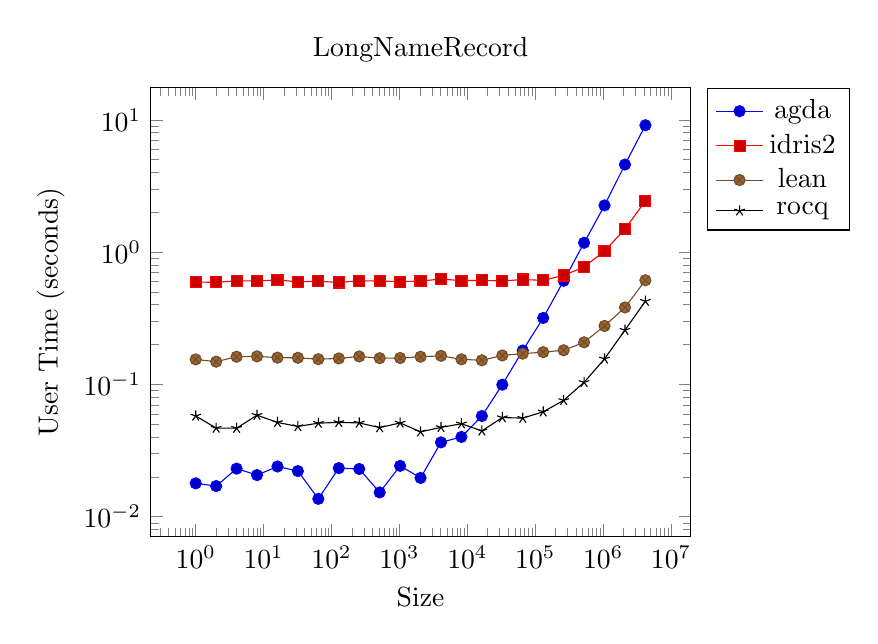
\begin{tikzpicture}
\begin{loglogaxis}
[title=LongNameRecord,
xlabel={Size},
ylabel={User Time (seconds)},
legend entries={agda,idris2,lean,rocq},
legend pos=outer north east,
]\addplot coordinates {
(4194304.0,9.097116) [0]
(2097152.0,4.588252) [0]
(1048576.0,2.253942) [0]
(524288.0,1.175644) [0]
(262144.0,0.606869) [0]
(131072.0,0.318102) [0]
(65536.0,0.180498) [0]
(32768.0,9.9566e-2) [0]
(16384.0,5.7703e-2) [0]
(8192.0,4.0103e-2) [0]
(4096.0,3.6509e-2) [0]
(2048.0,1.9649e-2) [0]
(1024.0,2.4239e-2) [0]
(512.0,1.5274e-2) [0]
(256.0,2.2951e-2) [0]
(128.0,2.3313e-2) [0]
(64.0,1.3655e-2) [0]
(32.0,2.2137e-2) [0]
(16.0,2.3973e-2) [0]
(8.0,2.0647e-2) [0]
(4.0,2.3102e-2) [0]
(2.0,1.7053e-2) [0]
(1.0,1.7885e-2) [0]
};
\addplot coordinates {
(4194304.0,2.435465) [0]
(2097152.0,1.494713) [0]
(1048576.0,1.018833) [0]
(524288.0,0.772144) [0]
(262144.0,0.66665) [0]
(131072.0,0.611889) [0]
(65536.0,0.620374) [0]
(32768.0,0.605496) [0]
(16384.0,0.611539) [0]
(8192.0,0.608788) [0]
(4096.0,0.626241) [0]
(2048.0,0.603874) [0]
(1024.0,0.598415) [0]
(512.0,0.604452) [0]
(256.0,0.60748) [0]
(128.0,0.589608) [0]
(64.0,0.603068) [0]
(32.0,0.596021) [0]
(16.0,0.616476) [0]
(8.0,0.605033) [0]
(4.0,0.606919) [0]
(2.0,0.591078) [0]
(1.0,0.594091) [0]
};
\addplot coordinates {
(4194304.0,0.612912) [0]
(2097152.0,0.381734) [0]
(1048576.0,0.276632) [0]
(524288.0,0.208152) [0]
(262144.0,0.181183) [0]
(131072.0,0.17531) [0]
(65536.0,0.170923) [0]
(32768.0,0.165527) [0]
(16384.0,0.15219) [0]
(8192.0,0.15478) [0]
(4096.0,0.164464) [0]
(2048.0,0.161915) [0]
(1024.0,0.158346) [0]
(512.0,0.157909) [0]
(256.0,0.162727) [0]
(128.0,0.157235) [0]
(64.0,0.155179) [0]
(32.0,0.158943) [0]
(16.0,0.159408) [0]
(8.0,0.162905) [0]
(4.0,0.16191) [0]
(2.0,0.148563) [0]
(1.0,0.15453) [0]
};
\addplot coordinates {
(4194304.0,0.426038) [0]
(2097152.0,0.257224) [0]
(1048576.0,0.156022) [0]
(524288.0,0.103696) [0]
(262144.0,7.5799e-2) [0]
(131072.0,6.2094e-2) [0]
(65536.0,5.5643e-2) [0]
(32768.0,5.6181e-2) [0]
(16384.0,4.4542e-2) [0]
(8192.0,5.0413e-2) [0]
(4096.0,4.7327e-2) [0]
(2048.0,4.3836e-2) [0]
(1024.0,5.1143e-2) [0]
(512.0,4.7186e-2) [0]
(256.0,5.1154e-2) [0]
(128.0,5.1667e-2) [0]
(64.0,5.0968e-2) [0]
(32.0,4.8123e-2) [0]
(16.0,5.1609e-2) [0]
(8.0,5.8562e-2) [0]
(4.0,4.6712e-2) [0]
(2.0,4.6796e-2) [0]
(1.0,5.7777e-2) [0]
};
\end{loglogaxis}
\end{tikzpicture}

% \\
% 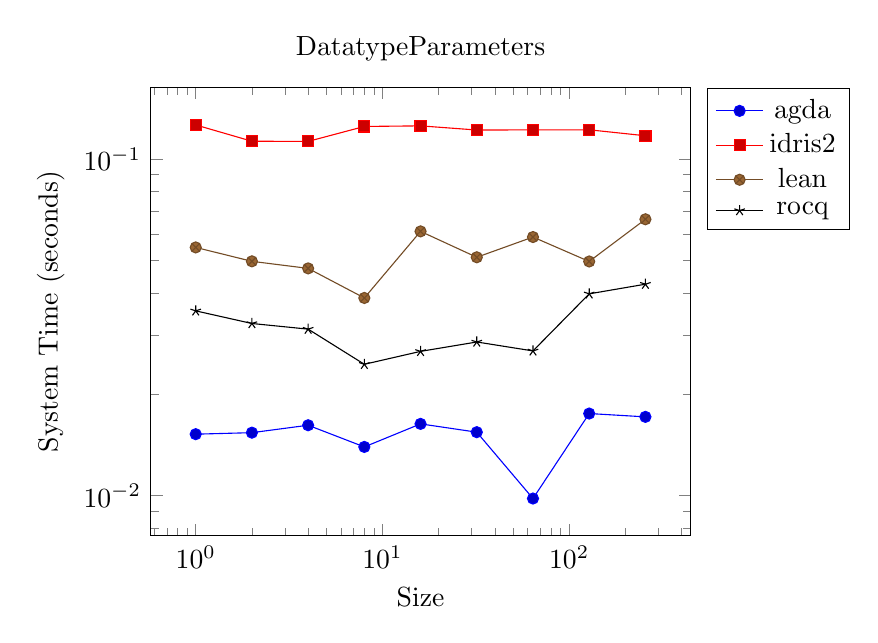
\begin{tikzpicture}
\begin{loglogaxis}
[title=DatatypeParameters,
xlabel={Size},
ylabel={System Time (seconds)},
legend entries={agda,idris2,lean,rocq},
legend pos=outer north east,
]\addplot coordinates {
(256.0,1.7155e-2) [0]
(128.0,1.755e-2) [0]
(64.0,9.813e-3) [0]
(32.0,1.545e-2) [0]
(16.0,1.6352e-2) [0]
(8.0,1.3967e-2) [0]
(4.0,1.62e-2) [0]
(2.0,1.5398e-2) [0]
(1.0,1.524e-2) [0]
};
\addplot coordinates {
(256.0,0.117316) [0]
(128.0,0.122186) [0]
(64.0,0.122117) [0]
(32.0,0.122001) [0]
(16.0,0.125521) [0]
(8.0,0.125017) [0]
(4.0,0.112862) [0]
(2.0,0.112996) [0]
(1.0,0.126323) [0]
};
\addplot coordinates {
(256.0,6.6273e-2) [256]
(128.0,4.9652e-2) [256]
(64.0,5.8684e-2) [0]
(32.0,5.1098e-2) [0]
(16.0,6.1002e-2) [0]
(8.0,3.8694e-2) [0]
(4.0,4.7356e-2) [0]
(2.0,4.9701e-2) [0]
(1.0,5.4661e-2) [0]
};
\addplot coordinates {
(256.0,4.2505e-2) [0]
(128.0,3.9801e-2) [0]
(64.0,2.6931e-2) [0]
(32.0,2.863e-2) [0]
(16.0,2.6848e-2) [0]
(8.0,2.4578e-2) [0]
(4.0,3.1258e-2) [0]
(2.0,3.2489e-2) [0]
(1.0,3.542e-2) [0]
};
\end{loglogaxis}
\end{tikzpicture}

% \\
% 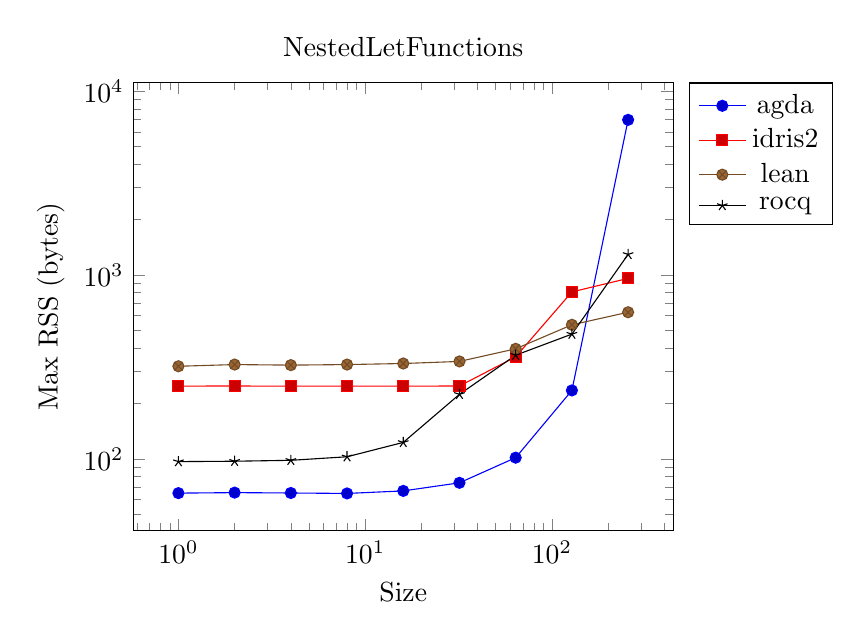
\begin{tikzpicture}
\begin{loglogaxis}
[title=NestedLetFunctions,
xlabel={Size},
ylabel={Max RSS (bytes)},
legend entries={agda,idris2,lean,rocq},
legend pos=outer north east,
]\addplot coordinates {
(256.0,6970.933248) [9]
(128.0,235.630592) [0]
(64.0,101.531648) [0]
(32.0,74.11712) [0]
(16.0,66.9696) [0]
(8.0,64.872448) [0]
(4.0,65.236992) [0]
(2.0,65.548288) [0]
(1.0,65.130496) [0]
};
\addplot coordinates {
(256.0,957.755392) [35072]
(128.0,808.771584) [35072]
(64.0,358.68672) [0]
(32.0,248.905728) [0]
(16.0,248.68864) [0]
(8.0,248.7296) [0]
(4.0,248.684544) [0]
(2.0,248.89344) [0]
(1.0,248.77056) [0]
};
\addplot coordinates {
(256.0,626.950144) [9]
(128.0,535.67488) [9]
(64.0,396.644352) [0]
(32.0,338.702336) [0]
(16.0,329.977856) [0]
(8.0,325.644288) [0]
(4.0,323.387392) [0]
(2.0,325.619712) [0]
(1.0,318.803968) [0]
};
\addplot coordinates {
(256.0,1293.410304) [0]
(128.0,476.749824) [0]
(64.0,366.256128) [0]
(32.0,224.354304) [0]
(16.0,122.884096) [0]
(8.0,102.670336) [0]
(4.0,98.213888) [0]
(2.0,97.087488) [0]
(1.0,96.620544) [0]
};
\end{loglogaxis}
\end{tikzpicture}


% \subsection{ConversionAddition}
% 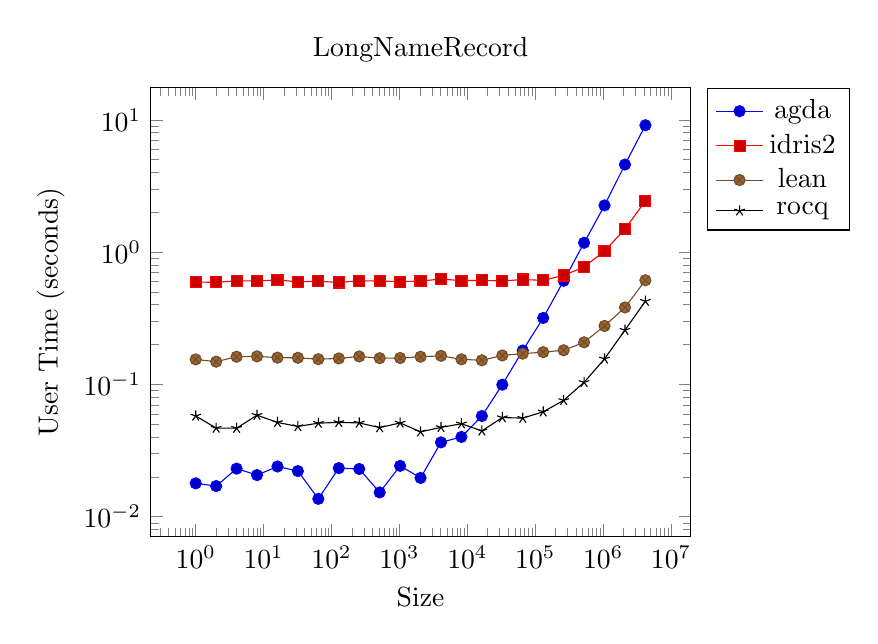
\begin{tikzpicture}
\begin{loglogaxis}
[title=LongNameRecord,
xlabel={Size},
ylabel={User Time (seconds)},
legend entries={agda,idris2,lean,rocq},
legend pos=outer north east,
]\addplot coordinates {
(4194304.0,9.097116) [0]
(2097152.0,4.588252) [0]
(1048576.0,2.253942) [0]
(524288.0,1.175644) [0]
(262144.0,0.606869) [0]
(131072.0,0.318102) [0]
(65536.0,0.180498) [0]
(32768.0,9.9566e-2) [0]
(16384.0,5.7703e-2) [0]
(8192.0,4.0103e-2) [0]
(4096.0,3.6509e-2) [0]
(2048.0,1.9649e-2) [0]
(1024.0,2.4239e-2) [0]
(512.0,1.5274e-2) [0]
(256.0,2.2951e-2) [0]
(128.0,2.3313e-2) [0]
(64.0,1.3655e-2) [0]
(32.0,2.2137e-2) [0]
(16.0,2.3973e-2) [0]
(8.0,2.0647e-2) [0]
(4.0,2.3102e-2) [0]
(2.0,1.7053e-2) [0]
(1.0,1.7885e-2) [0]
};
\addplot coordinates {
(4194304.0,2.435465) [0]
(2097152.0,1.494713) [0]
(1048576.0,1.018833) [0]
(524288.0,0.772144) [0]
(262144.0,0.66665) [0]
(131072.0,0.611889) [0]
(65536.0,0.620374) [0]
(32768.0,0.605496) [0]
(16384.0,0.611539) [0]
(8192.0,0.608788) [0]
(4096.0,0.626241) [0]
(2048.0,0.603874) [0]
(1024.0,0.598415) [0]
(512.0,0.604452) [0]
(256.0,0.60748) [0]
(128.0,0.589608) [0]
(64.0,0.603068) [0]
(32.0,0.596021) [0]
(16.0,0.616476) [0]
(8.0,0.605033) [0]
(4.0,0.606919) [0]
(2.0,0.591078) [0]
(1.0,0.594091) [0]
};
\addplot coordinates {
(4194304.0,0.612912) [0]
(2097152.0,0.381734) [0]
(1048576.0,0.276632) [0]
(524288.0,0.208152) [0]
(262144.0,0.181183) [0]
(131072.0,0.17531) [0]
(65536.0,0.170923) [0]
(32768.0,0.165527) [0]
(16384.0,0.15219) [0]
(8192.0,0.15478) [0]
(4096.0,0.164464) [0]
(2048.0,0.161915) [0]
(1024.0,0.158346) [0]
(512.0,0.157909) [0]
(256.0,0.162727) [0]
(128.0,0.157235) [0]
(64.0,0.155179) [0]
(32.0,0.158943) [0]
(16.0,0.159408) [0]
(8.0,0.162905) [0]
(4.0,0.16191) [0]
(2.0,0.148563) [0]
(1.0,0.15453) [0]
};
\addplot coordinates {
(4194304.0,0.426038) [0]
(2097152.0,0.257224) [0]
(1048576.0,0.156022) [0]
(524288.0,0.103696) [0]
(262144.0,7.5799e-2) [0]
(131072.0,6.2094e-2) [0]
(65536.0,5.5643e-2) [0]
(32768.0,5.6181e-2) [0]
(16384.0,4.4542e-2) [0]
(8192.0,5.0413e-2) [0]
(4096.0,4.7327e-2) [0]
(2048.0,4.3836e-2) [0]
(1024.0,5.1143e-2) [0]
(512.0,4.7186e-2) [0]
(256.0,5.1154e-2) [0]
(128.0,5.1667e-2) [0]
(64.0,5.0968e-2) [0]
(32.0,4.8123e-2) [0]
(16.0,5.1609e-2) [0]
(8.0,5.8562e-2) [0]
(4.0,4.6712e-2) [0]
(2.0,4.6796e-2) [0]
(1.0,5.7777e-2) [0]
};
\end{loglogaxis}
\end{tikzpicture}

% \\
% 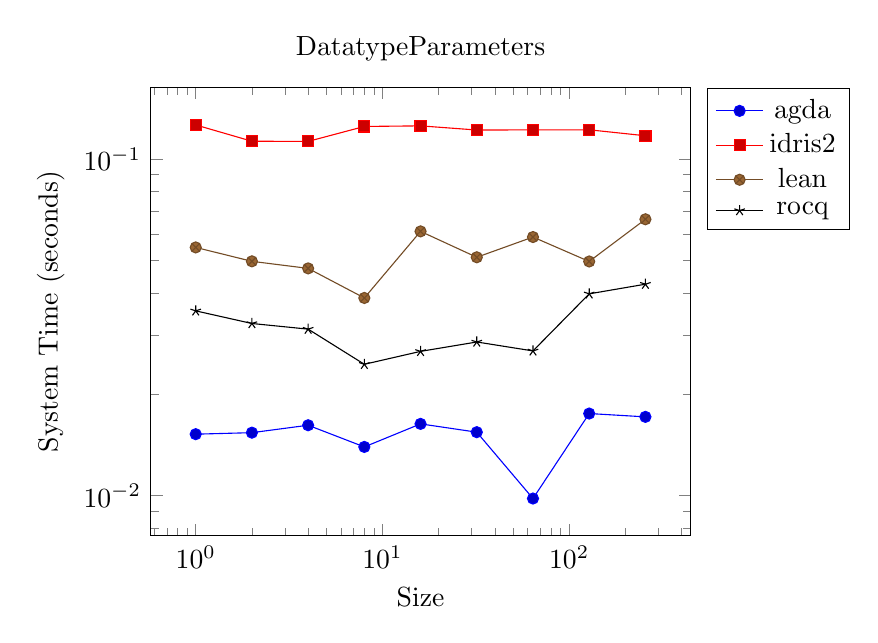
\begin{tikzpicture}
\begin{loglogaxis}
[title=DatatypeParameters,
xlabel={Size},
ylabel={System Time (seconds)},
legend entries={agda,idris2,lean,rocq},
legend pos=outer north east,
]\addplot coordinates {
(256.0,1.7155e-2) [0]
(128.0,1.755e-2) [0]
(64.0,9.813e-3) [0]
(32.0,1.545e-2) [0]
(16.0,1.6352e-2) [0]
(8.0,1.3967e-2) [0]
(4.0,1.62e-2) [0]
(2.0,1.5398e-2) [0]
(1.0,1.524e-2) [0]
};
\addplot coordinates {
(256.0,0.117316) [0]
(128.0,0.122186) [0]
(64.0,0.122117) [0]
(32.0,0.122001) [0]
(16.0,0.125521) [0]
(8.0,0.125017) [0]
(4.0,0.112862) [0]
(2.0,0.112996) [0]
(1.0,0.126323) [0]
};
\addplot coordinates {
(256.0,6.6273e-2) [256]
(128.0,4.9652e-2) [256]
(64.0,5.8684e-2) [0]
(32.0,5.1098e-2) [0]
(16.0,6.1002e-2) [0]
(8.0,3.8694e-2) [0]
(4.0,4.7356e-2) [0]
(2.0,4.9701e-2) [0]
(1.0,5.4661e-2) [0]
};
\addplot coordinates {
(256.0,4.2505e-2) [0]
(128.0,3.9801e-2) [0]
(64.0,2.6931e-2) [0]
(32.0,2.863e-2) [0]
(16.0,2.6848e-2) [0]
(8.0,2.4578e-2) [0]
(4.0,3.1258e-2) [0]
(2.0,3.2489e-2) [0]
(1.0,3.542e-2) [0]
};
\end{loglogaxis}
\end{tikzpicture}

% \\
% 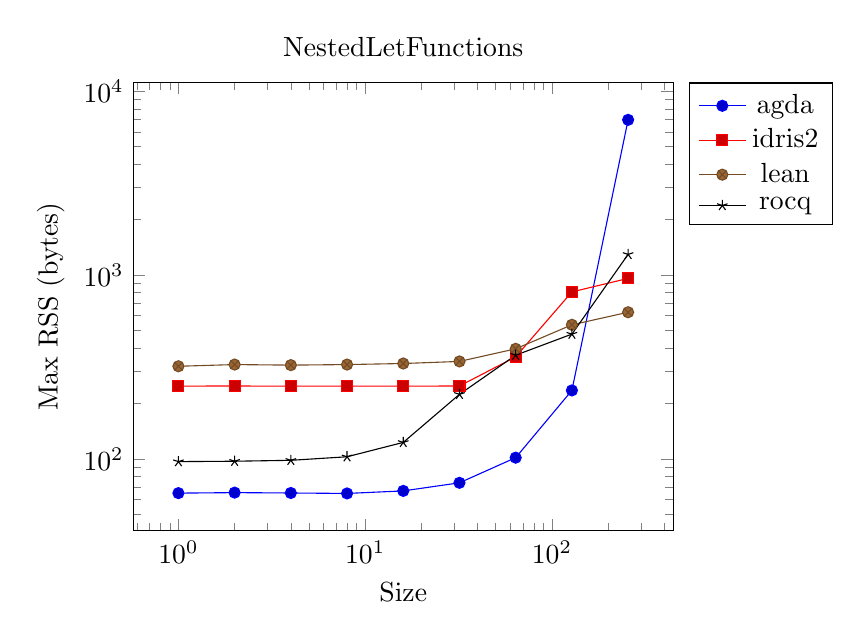
\begin{tikzpicture}
\begin{loglogaxis}
[title=NestedLetFunctions,
xlabel={Size},
ylabel={Max RSS (bytes)},
legend entries={agda,idris2,lean,rocq},
legend pos=outer north east,
]\addplot coordinates {
(256.0,6970.933248) [9]
(128.0,235.630592) [0]
(64.0,101.531648) [0]
(32.0,74.11712) [0]
(16.0,66.9696) [0]
(8.0,64.872448) [0]
(4.0,65.236992) [0]
(2.0,65.548288) [0]
(1.0,65.130496) [0]
};
\addplot coordinates {
(256.0,957.755392) [35072]
(128.0,808.771584) [35072]
(64.0,358.68672) [0]
(32.0,248.905728) [0]
(16.0,248.68864) [0]
(8.0,248.7296) [0]
(4.0,248.684544) [0]
(2.0,248.89344) [0]
(1.0,248.77056) [0]
};
\addplot coordinates {
(256.0,626.950144) [9]
(128.0,535.67488) [9]
(64.0,396.644352) [0]
(32.0,338.702336) [0]
(16.0,329.977856) [0]
(8.0,325.644288) [0]
(4.0,323.387392) [0]
(2.0,325.619712) [0]
(1.0,318.803968) [0]
};
\addplot coordinates {
(256.0,1293.410304) [0]
(128.0,476.749824) [0]
(64.0,366.256128) [0]
(32.0,224.354304) [0]
(16.0,122.884096) [0]
(8.0,102.670336) [0]
(4.0,98.213888) [0]
(2.0,97.087488) [0]
(1.0,96.620544) [0]
};
\end{loglogaxis}
\end{tikzpicture}


% \subsection{DatatypeParameters}
% 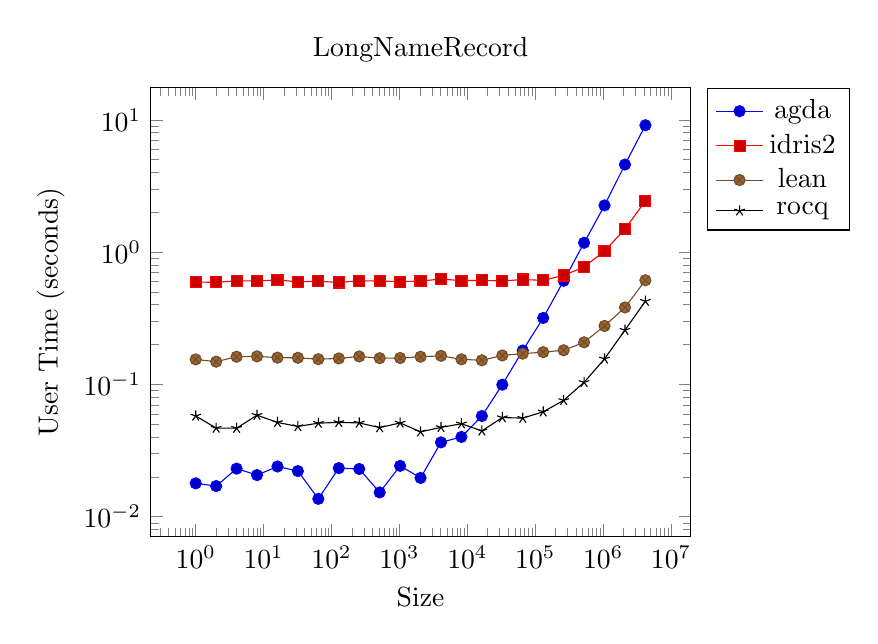
\begin{tikzpicture}
\begin{loglogaxis}
[title=LongNameRecord,
xlabel={Size},
ylabel={User Time (seconds)},
legend entries={agda,idris2,lean,rocq},
legend pos=outer north east,
]\addplot coordinates {
(4194304.0,9.097116) [0]
(2097152.0,4.588252) [0]
(1048576.0,2.253942) [0]
(524288.0,1.175644) [0]
(262144.0,0.606869) [0]
(131072.0,0.318102) [0]
(65536.0,0.180498) [0]
(32768.0,9.9566e-2) [0]
(16384.0,5.7703e-2) [0]
(8192.0,4.0103e-2) [0]
(4096.0,3.6509e-2) [0]
(2048.0,1.9649e-2) [0]
(1024.0,2.4239e-2) [0]
(512.0,1.5274e-2) [0]
(256.0,2.2951e-2) [0]
(128.0,2.3313e-2) [0]
(64.0,1.3655e-2) [0]
(32.0,2.2137e-2) [0]
(16.0,2.3973e-2) [0]
(8.0,2.0647e-2) [0]
(4.0,2.3102e-2) [0]
(2.0,1.7053e-2) [0]
(1.0,1.7885e-2) [0]
};
\addplot coordinates {
(4194304.0,2.435465) [0]
(2097152.0,1.494713) [0]
(1048576.0,1.018833) [0]
(524288.0,0.772144) [0]
(262144.0,0.66665) [0]
(131072.0,0.611889) [0]
(65536.0,0.620374) [0]
(32768.0,0.605496) [0]
(16384.0,0.611539) [0]
(8192.0,0.608788) [0]
(4096.0,0.626241) [0]
(2048.0,0.603874) [0]
(1024.0,0.598415) [0]
(512.0,0.604452) [0]
(256.0,0.60748) [0]
(128.0,0.589608) [0]
(64.0,0.603068) [0]
(32.0,0.596021) [0]
(16.0,0.616476) [0]
(8.0,0.605033) [0]
(4.0,0.606919) [0]
(2.0,0.591078) [0]
(1.0,0.594091) [0]
};
\addplot coordinates {
(4194304.0,0.612912) [0]
(2097152.0,0.381734) [0]
(1048576.0,0.276632) [0]
(524288.0,0.208152) [0]
(262144.0,0.181183) [0]
(131072.0,0.17531) [0]
(65536.0,0.170923) [0]
(32768.0,0.165527) [0]
(16384.0,0.15219) [0]
(8192.0,0.15478) [0]
(4096.0,0.164464) [0]
(2048.0,0.161915) [0]
(1024.0,0.158346) [0]
(512.0,0.157909) [0]
(256.0,0.162727) [0]
(128.0,0.157235) [0]
(64.0,0.155179) [0]
(32.0,0.158943) [0]
(16.0,0.159408) [0]
(8.0,0.162905) [0]
(4.0,0.16191) [0]
(2.0,0.148563) [0]
(1.0,0.15453) [0]
};
\addplot coordinates {
(4194304.0,0.426038) [0]
(2097152.0,0.257224) [0]
(1048576.0,0.156022) [0]
(524288.0,0.103696) [0]
(262144.0,7.5799e-2) [0]
(131072.0,6.2094e-2) [0]
(65536.0,5.5643e-2) [0]
(32768.0,5.6181e-2) [0]
(16384.0,4.4542e-2) [0]
(8192.0,5.0413e-2) [0]
(4096.0,4.7327e-2) [0]
(2048.0,4.3836e-2) [0]
(1024.0,5.1143e-2) [0]
(512.0,4.7186e-2) [0]
(256.0,5.1154e-2) [0]
(128.0,5.1667e-2) [0]
(64.0,5.0968e-2) [0]
(32.0,4.8123e-2) [0]
(16.0,5.1609e-2) [0]
(8.0,5.8562e-2) [0]
(4.0,4.6712e-2) [0]
(2.0,4.6796e-2) [0]
(1.0,5.7777e-2) [0]
};
\end{loglogaxis}
\end{tikzpicture}

% \\
% 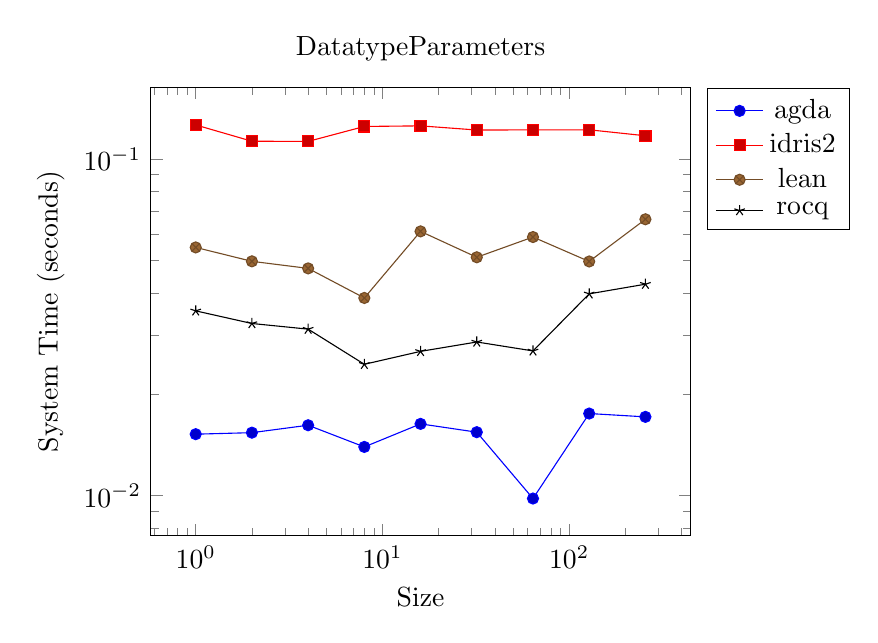
\begin{tikzpicture}
\begin{loglogaxis}
[title=DatatypeParameters,
xlabel={Size},
ylabel={System Time (seconds)},
legend entries={agda,idris2,lean,rocq},
legend pos=outer north east,
]\addplot coordinates {
(256.0,1.7155e-2) [0]
(128.0,1.755e-2) [0]
(64.0,9.813e-3) [0]
(32.0,1.545e-2) [0]
(16.0,1.6352e-2) [0]
(8.0,1.3967e-2) [0]
(4.0,1.62e-2) [0]
(2.0,1.5398e-2) [0]
(1.0,1.524e-2) [0]
};
\addplot coordinates {
(256.0,0.117316) [0]
(128.0,0.122186) [0]
(64.0,0.122117) [0]
(32.0,0.122001) [0]
(16.0,0.125521) [0]
(8.0,0.125017) [0]
(4.0,0.112862) [0]
(2.0,0.112996) [0]
(1.0,0.126323) [0]
};
\addplot coordinates {
(256.0,6.6273e-2) [256]
(128.0,4.9652e-2) [256]
(64.0,5.8684e-2) [0]
(32.0,5.1098e-2) [0]
(16.0,6.1002e-2) [0]
(8.0,3.8694e-2) [0]
(4.0,4.7356e-2) [0]
(2.0,4.9701e-2) [0]
(1.0,5.4661e-2) [0]
};
\addplot coordinates {
(256.0,4.2505e-2) [0]
(128.0,3.9801e-2) [0]
(64.0,2.6931e-2) [0]
(32.0,2.863e-2) [0]
(16.0,2.6848e-2) [0]
(8.0,2.4578e-2) [0]
(4.0,3.1258e-2) [0]
(2.0,3.2489e-2) [0]
(1.0,3.542e-2) [0]
};
\end{loglogaxis}
\end{tikzpicture}

% \\
% 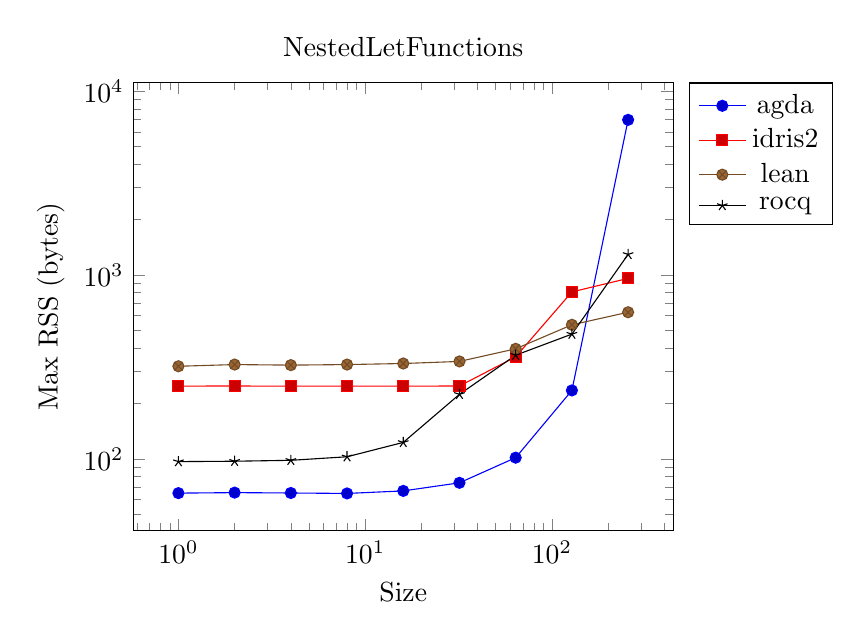
\begin{tikzpicture}
\begin{loglogaxis}
[title=NestedLetFunctions,
xlabel={Size},
ylabel={Max RSS (bytes)},
legend entries={agda,idris2,lean,rocq},
legend pos=outer north east,
]\addplot coordinates {
(256.0,6970.933248) [9]
(128.0,235.630592) [0]
(64.0,101.531648) [0]
(32.0,74.11712) [0]
(16.0,66.9696) [0]
(8.0,64.872448) [0]
(4.0,65.236992) [0]
(2.0,65.548288) [0]
(1.0,65.130496) [0]
};
\addplot coordinates {
(256.0,957.755392) [35072]
(128.0,808.771584) [35072]
(64.0,358.68672) [0]
(32.0,248.905728) [0]
(16.0,248.68864) [0]
(8.0,248.7296) [0]
(4.0,248.684544) [0]
(2.0,248.89344) [0]
(1.0,248.77056) [0]
};
\addplot coordinates {
(256.0,626.950144) [9]
(128.0,535.67488) [9]
(64.0,396.644352) [0]
(32.0,338.702336) [0]
(16.0,329.977856) [0]
(8.0,325.644288) [0]
(4.0,323.387392) [0]
(2.0,325.619712) [0]
(1.0,318.803968) [0]
};
\addplot coordinates {
(256.0,1293.410304) [0]
(128.0,476.749824) [0]
(64.0,366.256128) [0]
(32.0,224.354304) [0]
(16.0,122.884096) [0]
(8.0,102.670336) [0]
(4.0,98.213888) [0]
(2.0,97.087488) [0]
(1.0,96.620544) [0]
};
\end{loglogaxis}
\end{tikzpicture}


% \subsection{IdChain}
% 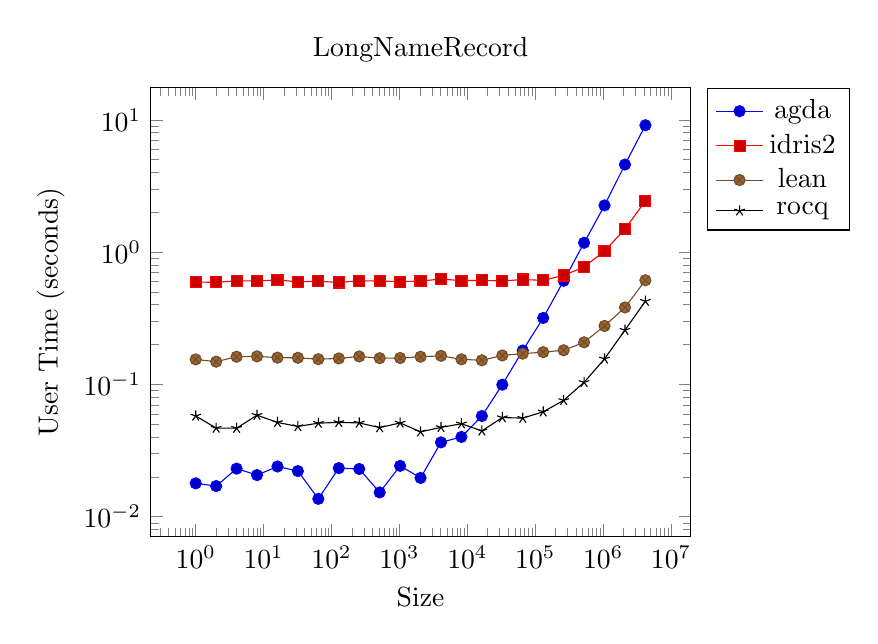
\begin{tikzpicture}
\begin{loglogaxis}
[title=LongNameRecord,
xlabel={Size},
ylabel={User Time (seconds)},
legend entries={agda,idris2,lean,rocq},
legend pos=outer north east,
]\addplot coordinates {
(4194304.0,9.097116) [0]
(2097152.0,4.588252) [0]
(1048576.0,2.253942) [0]
(524288.0,1.175644) [0]
(262144.0,0.606869) [0]
(131072.0,0.318102) [0]
(65536.0,0.180498) [0]
(32768.0,9.9566e-2) [0]
(16384.0,5.7703e-2) [0]
(8192.0,4.0103e-2) [0]
(4096.0,3.6509e-2) [0]
(2048.0,1.9649e-2) [0]
(1024.0,2.4239e-2) [0]
(512.0,1.5274e-2) [0]
(256.0,2.2951e-2) [0]
(128.0,2.3313e-2) [0]
(64.0,1.3655e-2) [0]
(32.0,2.2137e-2) [0]
(16.0,2.3973e-2) [0]
(8.0,2.0647e-2) [0]
(4.0,2.3102e-2) [0]
(2.0,1.7053e-2) [0]
(1.0,1.7885e-2) [0]
};
\addplot coordinates {
(4194304.0,2.435465) [0]
(2097152.0,1.494713) [0]
(1048576.0,1.018833) [0]
(524288.0,0.772144) [0]
(262144.0,0.66665) [0]
(131072.0,0.611889) [0]
(65536.0,0.620374) [0]
(32768.0,0.605496) [0]
(16384.0,0.611539) [0]
(8192.0,0.608788) [0]
(4096.0,0.626241) [0]
(2048.0,0.603874) [0]
(1024.0,0.598415) [0]
(512.0,0.604452) [0]
(256.0,0.60748) [0]
(128.0,0.589608) [0]
(64.0,0.603068) [0]
(32.0,0.596021) [0]
(16.0,0.616476) [0]
(8.0,0.605033) [0]
(4.0,0.606919) [0]
(2.0,0.591078) [0]
(1.0,0.594091) [0]
};
\addplot coordinates {
(4194304.0,0.612912) [0]
(2097152.0,0.381734) [0]
(1048576.0,0.276632) [0]
(524288.0,0.208152) [0]
(262144.0,0.181183) [0]
(131072.0,0.17531) [0]
(65536.0,0.170923) [0]
(32768.0,0.165527) [0]
(16384.0,0.15219) [0]
(8192.0,0.15478) [0]
(4096.0,0.164464) [0]
(2048.0,0.161915) [0]
(1024.0,0.158346) [0]
(512.0,0.157909) [0]
(256.0,0.162727) [0]
(128.0,0.157235) [0]
(64.0,0.155179) [0]
(32.0,0.158943) [0]
(16.0,0.159408) [0]
(8.0,0.162905) [0]
(4.0,0.16191) [0]
(2.0,0.148563) [0]
(1.0,0.15453) [0]
};
\addplot coordinates {
(4194304.0,0.426038) [0]
(2097152.0,0.257224) [0]
(1048576.0,0.156022) [0]
(524288.0,0.103696) [0]
(262144.0,7.5799e-2) [0]
(131072.0,6.2094e-2) [0]
(65536.0,5.5643e-2) [0]
(32768.0,5.6181e-2) [0]
(16384.0,4.4542e-2) [0]
(8192.0,5.0413e-2) [0]
(4096.0,4.7327e-2) [0]
(2048.0,4.3836e-2) [0]
(1024.0,5.1143e-2) [0]
(512.0,4.7186e-2) [0]
(256.0,5.1154e-2) [0]
(128.0,5.1667e-2) [0]
(64.0,5.0968e-2) [0]
(32.0,4.8123e-2) [0]
(16.0,5.1609e-2) [0]
(8.0,5.8562e-2) [0]
(4.0,4.6712e-2) [0]
(2.0,4.6796e-2) [0]
(1.0,5.7777e-2) [0]
};
\end{loglogaxis}
\end{tikzpicture}

% \\
% 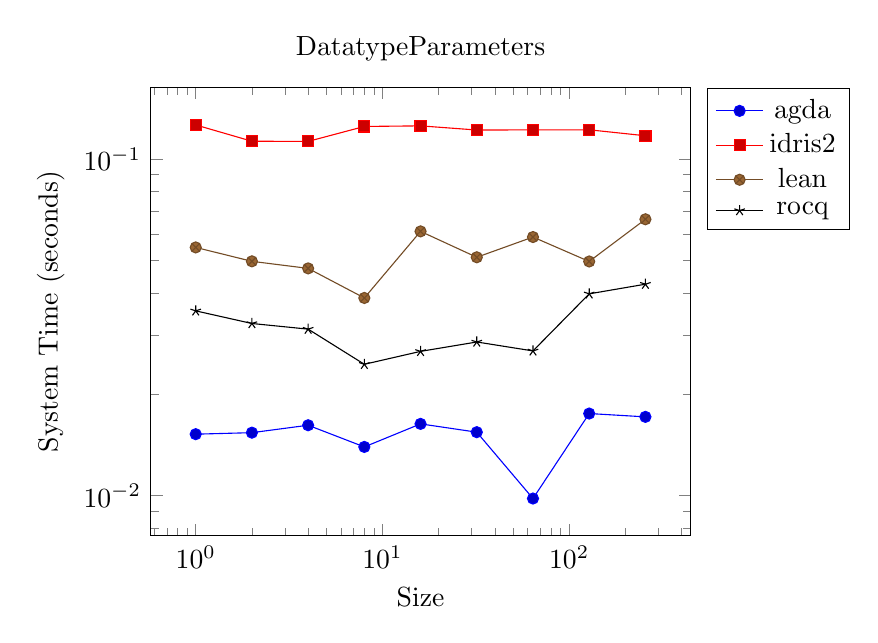
\begin{tikzpicture}
\begin{loglogaxis}
[title=DatatypeParameters,
xlabel={Size},
ylabel={System Time (seconds)},
legend entries={agda,idris2,lean,rocq},
legend pos=outer north east,
]\addplot coordinates {
(256.0,1.7155e-2) [0]
(128.0,1.755e-2) [0]
(64.0,9.813e-3) [0]
(32.0,1.545e-2) [0]
(16.0,1.6352e-2) [0]
(8.0,1.3967e-2) [0]
(4.0,1.62e-2) [0]
(2.0,1.5398e-2) [0]
(1.0,1.524e-2) [0]
};
\addplot coordinates {
(256.0,0.117316) [0]
(128.0,0.122186) [0]
(64.0,0.122117) [0]
(32.0,0.122001) [0]
(16.0,0.125521) [0]
(8.0,0.125017) [0]
(4.0,0.112862) [0]
(2.0,0.112996) [0]
(1.0,0.126323) [0]
};
\addplot coordinates {
(256.0,6.6273e-2) [256]
(128.0,4.9652e-2) [256]
(64.0,5.8684e-2) [0]
(32.0,5.1098e-2) [0]
(16.0,6.1002e-2) [0]
(8.0,3.8694e-2) [0]
(4.0,4.7356e-2) [0]
(2.0,4.9701e-2) [0]
(1.0,5.4661e-2) [0]
};
\addplot coordinates {
(256.0,4.2505e-2) [0]
(128.0,3.9801e-2) [0]
(64.0,2.6931e-2) [0]
(32.0,2.863e-2) [0]
(16.0,2.6848e-2) [0]
(8.0,2.4578e-2) [0]
(4.0,3.1258e-2) [0]
(2.0,3.2489e-2) [0]
(1.0,3.542e-2) [0]
};
\end{loglogaxis}
\end{tikzpicture}

% \\
% 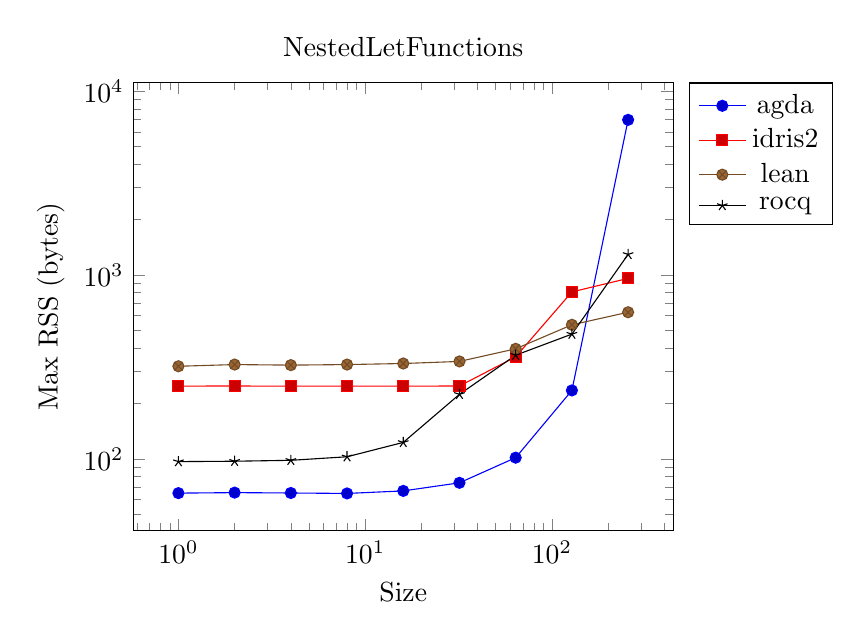
\begin{tikzpicture}
\begin{loglogaxis}
[title=NestedLetFunctions,
xlabel={Size},
ylabel={Max RSS (bytes)},
legend entries={agda,idris2,lean,rocq},
legend pos=outer north east,
]\addplot coordinates {
(256.0,6970.933248) [9]
(128.0,235.630592) [0]
(64.0,101.531648) [0]
(32.0,74.11712) [0]
(16.0,66.9696) [0]
(8.0,64.872448) [0]
(4.0,65.236992) [0]
(2.0,65.548288) [0]
(1.0,65.130496) [0]
};
\addplot coordinates {
(256.0,957.755392) [35072]
(128.0,808.771584) [35072]
(64.0,358.68672) [0]
(32.0,248.905728) [0]
(16.0,248.68864) [0]
(8.0,248.7296) [0]
(4.0,248.684544) [0]
(2.0,248.89344) [0]
(1.0,248.77056) [0]
};
\addplot coordinates {
(256.0,626.950144) [9]
(128.0,535.67488) [9]
(64.0,396.644352) [0]
(32.0,338.702336) [0]
(16.0,329.977856) [0]
(8.0,325.644288) [0]
(4.0,323.387392) [0]
(2.0,325.619712) [0]
(1.0,318.803968) [0]
};
\addplot coordinates {
(256.0,1293.410304) [0]
(128.0,476.749824) [0]
(64.0,366.256128) [0]
(32.0,224.354304) [0]
(16.0,122.884096) [0]
(8.0,102.670336) [0]
(4.0,98.213888) [0]
(2.0,97.087488) [0]
(1.0,96.620544) [0]
};
\end{loglogaxis}
\end{tikzpicture}


% \subsection{LargeDependentRecord}
% 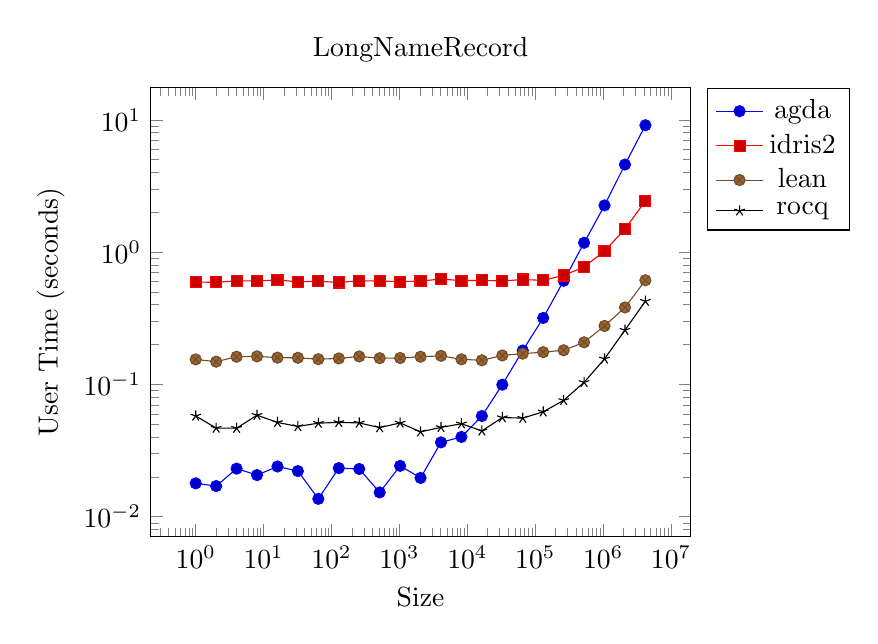
\begin{tikzpicture}
\begin{loglogaxis}
[title=LongNameRecord,
xlabel={Size},
ylabel={User Time (seconds)},
legend entries={agda,idris2,lean,rocq},
legend pos=outer north east,
]\addplot coordinates {
(4194304.0,9.097116) [0]
(2097152.0,4.588252) [0]
(1048576.0,2.253942) [0]
(524288.0,1.175644) [0]
(262144.0,0.606869) [0]
(131072.0,0.318102) [0]
(65536.0,0.180498) [0]
(32768.0,9.9566e-2) [0]
(16384.0,5.7703e-2) [0]
(8192.0,4.0103e-2) [0]
(4096.0,3.6509e-2) [0]
(2048.0,1.9649e-2) [0]
(1024.0,2.4239e-2) [0]
(512.0,1.5274e-2) [0]
(256.0,2.2951e-2) [0]
(128.0,2.3313e-2) [0]
(64.0,1.3655e-2) [0]
(32.0,2.2137e-2) [0]
(16.0,2.3973e-2) [0]
(8.0,2.0647e-2) [0]
(4.0,2.3102e-2) [0]
(2.0,1.7053e-2) [0]
(1.0,1.7885e-2) [0]
};
\addplot coordinates {
(4194304.0,2.435465) [0]
(2097152.0,1.494713) [0]
(1048576.0,1.018833) [0]
(524288.0,0.772144) [0]
(262144.0,0.66665) [0]
(131072.0,0.611889) [0]
(65536.0,0.620374) [0]
(32768.0,0.605496) [0]
(16384.0,0.611539) [0]
(8192.0,0.608788) [0]
(4096.0,0.626241) [0]
(2048.0,0.603874) [0]
(1024.0,0.598415) [0]
(512.0,0.604452) [0]
(256.0,0.60748) [0]
(128.0,0.589608) [0]
(64.0,0.603068) [0]
(32.0,0.596021) [0]
(16.0,0.616476) [0]
(8.0,0.605033) [0]
(4.0,0.606919) [0]
(2.0,0.591078) [0]
(1.0,0.594091) [0]
};
\addplot coordinates {
(4194304.0,0.612912) [0]
(2097152.0,0.381734) [0]
(1048576.0,0.276632) [0]
(524288.0,0.208152) [0]
(262144.0,0.181183) [0]
(131072.0,0.17531) [0]
(65536.0,0.170923) [0]
(32768.0,0.165527) [0]
(16384.0,0.15219) [0]
(8192.0,0.15478) [0]
(4096.0,0.164464) [0]
(2048.0,0.161915) [0]
(1024.0,0.158346) [0]
(512.0,0.157909) [0]
(256.0,0.162727) [0]
(128.0,0.157235) [0]
(64.0,0.155179) [0]
(32.0,0.158943) [0]
(16.0,0.159408) [0]
(8.0,0.162905) [0]
(4.0,0.16191) [0]
(2.0,0.148563) [0]
(1.0,0.15453) [0]
};
\addplot coordinates {
(4194304.0,0.426038) [0]
(2097152.0,0.257224) [0]
(1048576.0,0.156022) [0]
(524288.0,0.103696) [0]
(262144.0,7.5799e-2) [0]
(131072.0,6.2094e-2) [0]
(65536.0,5.5643e-2) [0]
(32768.0,5.6181e-2) [0]
(16384.0,4.4542e-2) [0]
(8192.0,5.0413e-2) [0]
(4096.0,4.7327e-2) [0]
(2048.0,4.3836e-2) [0]
(1024.0,5.1143e-2) [0]
(512.0,4.7186e-2) [0]
(256.0,5.1154e-2) [0]
(128.0,5.1667e-2) [0]
(64.0,5.0968e-2) [0]
(32.0,4.8123e-2) [0]
(16.0,5.1609e-2) [0]
(8.0,5.8562e-2) [0]
(4.0,4.6712e-2) [0]
(2.0,4.6796e-2) [0]
(1.0,5.7777e-2) [0]
};
\end{loglogaxis}
\end{tikzpicture}

% \\
% 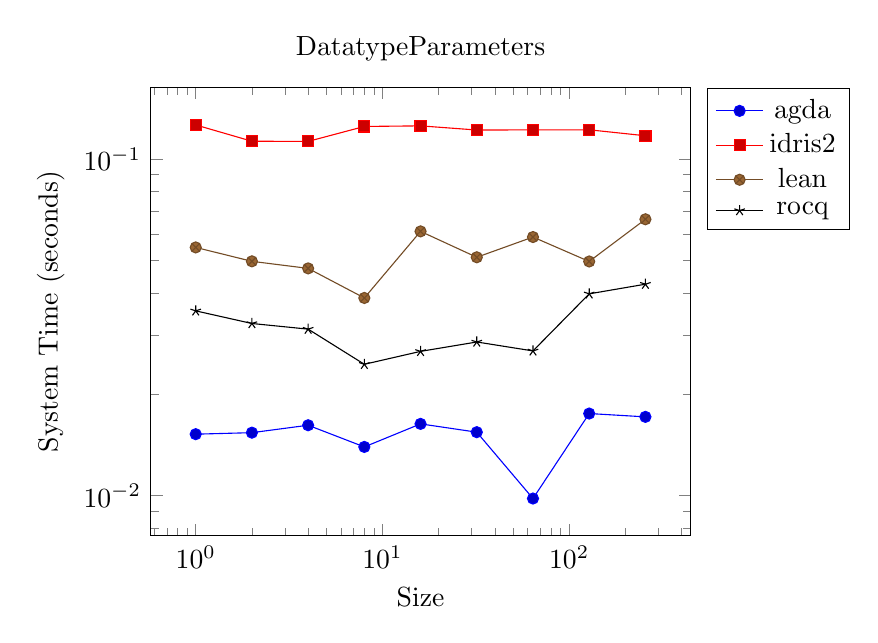
\begin{tikzpicture}
\begin{loglogaxis}
[title=DatatypeParameters,
xlabel={Size},
ylabel={System Time (seconds)},
legend entries={agda,idris2,lean,rocq},
legend pos=outer north east,
]\addplot coordinates {
(256.0,1.7155e-2) [0]
(128.0,1.755e-2) [0]
(64.0,9.813e-3) [0]
(32.0,1.545e-2) [0]
(16.0,1.6352e-2) [0]
(8.0,1.3967e-2) [0]
(4.0,1.62e-2) [0]
(2.0,1.5398e-2) [0]
(1.0,1.524e-2) [0]
};
\addplot coordinates {
(256.0,0.117316) [0]
(128.0,0.122186) [0]
(64.0,0.122117) [0]
(32.0,0.122001) [0]
(16.0,0.125521) [0]
(8.0,0.125017) [0]
(4.0,0.112862) [0]
(2.0,0.112996) [0]
(1.0,0.126323) [0]
};
\addplot coordinates {
(256.0,6.6273e-2) [256]
(128.0,4.9652e-2) [256]
(64.0,5.8684e-2) [0]
(32.0,5.1098e-2) [0]
(16.0,6.1002e-2) [0]
(8.0,3.8694e-2) [0]
(4.0,4.7356e-2) [0]
(2.0,4.9701e-2) [0]
(1.0,5.4661e-2) [0]
};
\addplot coordinates {
(256.0,4.2505e-2) [0]
(128.0,3.9801e-2) [0]
(64.0,2.6931e-2) [0]
(32.0,2.863e-2) [0]
(16.0,2.6848e-2) [0]
(8.0,2.4578e-2) [0]
(4.0,3.1258e-2) [0]
(2.0,3.2489e-2) [0]
(1.0,3.542e-2) [0]
};
\end{loglogaxis}
\end{tikzpicture}

% \\
% 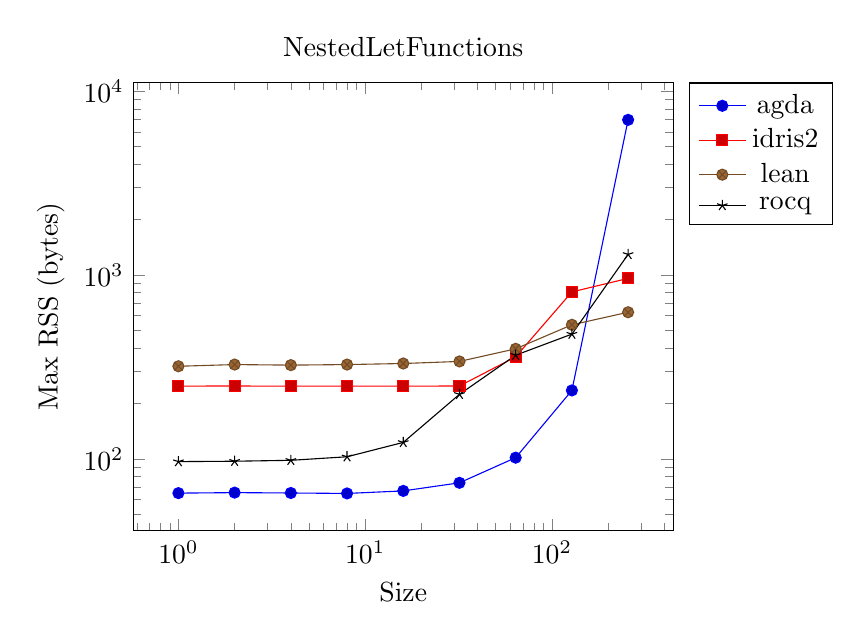
\begin{tikzpicture}
\begin{loglogaxis}
[title=NestedLetFunctions,
xlabel={Size},
ylabel={Max RSS (bytes)},
legend entries={agda,idris2,lean,rocq},
legend pos=outer north east,
]\addplot coordinates {
(256.0,6970.933248) [9]
(128.0,235.630592) [0]
(64.0,101.531648) [0]
(32.0,74.11712) [0]
(16.0,66.9696) [0]
(8.0,64.872448) [0]
(4.0,65.236992) [0]
(2.0,65.548288) [0]
(1.0,65.130496) [0]
};
\addplot coordinates {
(256.0,957.755392) [35072]
(128.0,808.771584) [35072]
(64.0,358.68672) [0]
(32.0,248.905728) [0]
(16.0,248.68864) [0]
(8.0,248.7296) [0]
(4.0,248.684544) [0]
(2.0,248.89344) [0]
(1.0,248.77056) [0]
};
\addplot coordinates {
(256.0,626.950144) [9]
(128.0,535.67488) [9]
(64.0,396.644352) [0]
(32.0,338.702336) [0]
(16.0,329.977856) [0]
(8.0,325.644288) [0]
(4.0,323.387392) [0]
(2.0,325.619712) [0]
(1.0,318.803968) [0]
};
\addplot coordinates {
(256.0,1293.410304) [0]
(128.0,476.749824) [0]
(64.0,366.256128) [0]
(32.0,224.354304) [0]
(16.0,122.884096) [0]
(8.0,102.670336) [0]
(4.0,98.213888) [0]
(2.0,97.087488) [0]
(1.0,96.620544) [0]
};
\end{loglogaxis}
\end{tikzpicture}


% \subsection{LargeIndexedDatatype}
% 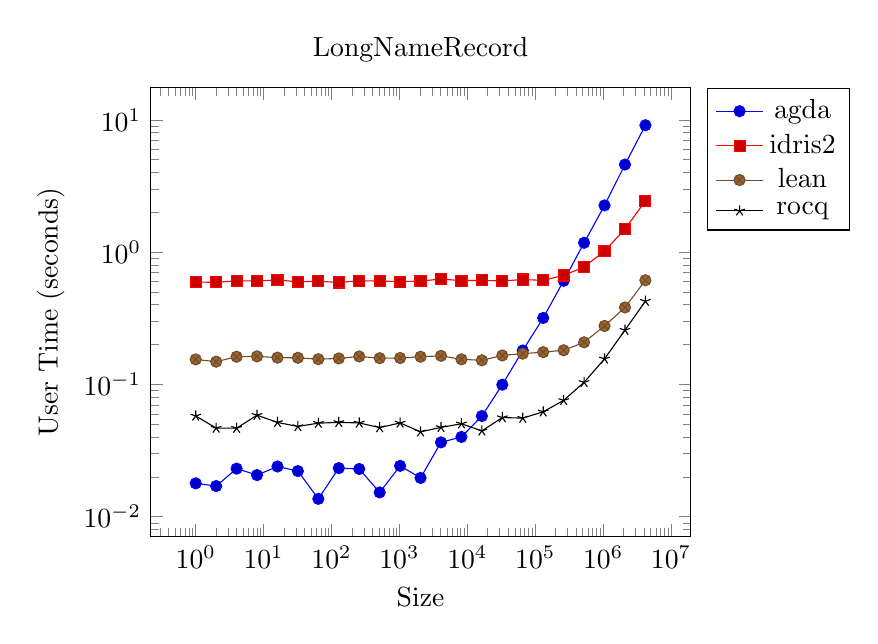
\begin{tikzpicture}
\begin{loglogaxis}
[title=LongNameRecord,
xlabel={Size},
ylabel={User Time (seconds)},
legend entries={agda,idris2,lean,rocq},
legend pos=outer north east,
]\addplot coordinates {
(4194304.0,9.097116) [0]
(2097152.0,4.588252) [0]
(1048576.0,2.253942) [0]
(524288.0,1.175644) [0]
(262144.0,0.606869) [0]
(131072.0,0.318102) [0]
(65536.0,0.180498) [0]
(32768.0,9.9566e-2) [0]
(16384.0,5.7703e-2) [0]
(8192.0,4.0103e-2) [0]
(4096.0,3.6509e-2) [0]
(2048.0,1.9649e-2) [0]
(1024.0,2.4239e-2) [0]
(512.0,1.5274e-2) [0]
(256.0,2.2951e-2) [0]
(128.0,2.3313e-2) [0]
(64.0,1.3655e-2) [0]
(32.0,2.2137e-2) [0]
(16.0,2.3973e-2) [0]
(8.0,2.0647e-2) [0]
(4.0,2.3102e-2) [0]
(2.0,1.7053e-2) [0]
(1.0,1.7885e-2) [0]
};
\addplot coordinates {
(4194304.0,2.435465) [0]
(2097152.0,1.494713) [0]
(1048576.0,1.018833) [0]
(524288.0,0.772144) [0]
(262144.0,0.66665) [0]
(131072.0,0.611889) [0]
(65536.0,0.620374) [0]
(32768.0,0.605496) [0]
(16384.0,0.611539) [0]
(8192.0,0.608788) [0]
(4096.0,0.626241) [0]
(2048.0,0.603874) [0]
(1024.0,0.598415) [0]
(512.0,0.604452) [0]
(256.0,0.60748) [0]
(128.0,0.589608) [0]
(64.0,0.603068) [0]
(32.0,0.596021) [0]
(16.0,0.616476) [0]
(8.0,0.605033) [0]
(4.0,0.606919) [0]
(2.0,0.591078) [0]
(1.0,0.594091) [0]
};
\addplot coordinates {
(4194304.0,0.612912) [0]
(2097152.0,0.381734) [0]
(1048576.0,0.276632) [0]
(524288.0,0.208152) [0]
(262144.0,0.181183) [0]
(131072.0,0.17531) [0]
(65536.0,0.170923) [0]
(32768.0,0.165527) [0]
(16384.0,0.15219) [0]
(8192.0,0.15478) [0]
(4096.0,0.164464) [0]
(2048.0,0.161915) [0]
(1024.0,0.158346) [0]
(512.0,0.157909) [0]
(256.0,0.162727) [0]
(128.0,0.157235) [0]
(64.0,0.155179) [0]
(32.0,0.158943) [0]
(16.0,0.159408) [0]
(8.0,0.162905) [0]
(4.0,0.16191) [0]
(2.0,0.148563) [0]
(1.0,0.15453) [0]
};
\addplot coordinates {
(4194304.0,0.426038) [0]
(2097152.0,0.257224) [0]
(1048576.0,0.156022) [0]
(524288.0,0.103696) [0]
(262144.0,7.5799e-2) [0]
(131072.0,6.2094e-2) [0]
(65536.0,5.5643e-2) [0]
(32768.0,5.6181e-2) [0]
(16384.0,4.4542e-2) [0]
(8192.0,5.0413e-2) [0]
(4096.0,4.7327e-2) [0]
(2048.0,4.3836e-2) [0]
(1024.0,5.1143e-2) [0]
(512.0,4.7186e-2) [0]
(256.0,5.1154e-2) [0]
(128.0,5.1667e-2) [0]
(64.0,5.0968e-2) [0]
(32.0,4.8123e-2) [0]
(16.0,5.1609e-2) [0]
(8.0,5.8562e-2) [0]
(4.0,4.6712e-2) [0]
(2.0,4.6796e-2) [0]
(1.0,5.7777e-2) [0]
};
\end{loglogaxis}
\end{tikzpicture}

% \\
% 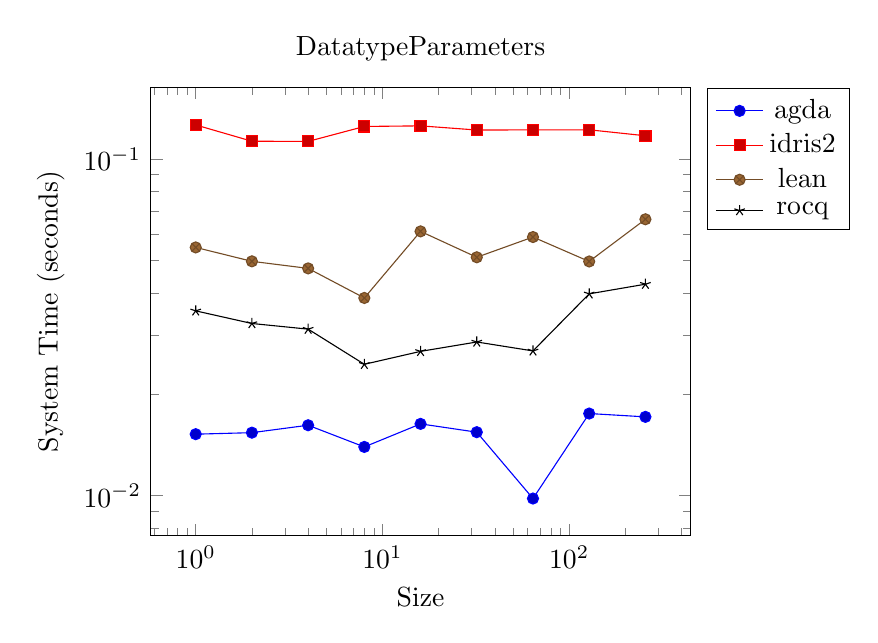
\begin{tikzpicture}
\begin{loglogaxis}
[title=DatatypeParameters,
xlabel={Size},
ylabel={System Time (seconds)},
legend entries={agda,idris2,lean,rocq},
legend pos=outer north east,
]\addplot coordinates {
(256.0,1.7155e-2) [0]
(128.0,1.755e-2) [0]
(64.0,9.813e-3) [0]
(32.0,1.545e-2) [0]
(16.0,1.6352e-2) [0]
(8.0,1.3967e-2) [0]
(4.0,1.62e-2) [0]
(2.0,1.5398e-2) [0]
(1.0,1.524e-2) [0]
};
\addplot coordinates {
(256.0,0.117316) [0]
(128.0,0.122186) [0]
(64.0,0.122117) [0]
(32.0,0.122001) [0]
(16.0,0.125521) [0]
(8.0,0.125017) [0]
(4.0,0.112862) [0]
(2.0,0.112996) [0]
(1.0,0.126323) [0]
};
\addplot coordinates {
(256.0,6.6273e-2) [256]
(128.0,4.9652e-2) [256]
(64.0,5.8684e-2) [0]
(32.0,5.1098e-2) [0]
(16.0,6.1002e-2) [0]
(8.0,3.8694e-2) [0]
(4.0,4.7356e-2) [0]
(2.0,4.9701e-2) [0]
(1.0,5.4661e-2) [0]
};
\addplot coordinates {
(256.0,4.2505e-2) [0]
(128.0,3.9801e-2) [0]
(64.0,2.6931e-2) [0]
(32.0,2.863e-2) [0]
(16.0,2.6848e-2) [0]
(8.0,2.4578e-2) [0]
(4.0,3.1258e-2) [0]
(2.0,3.2489e-2) [0]
(1.0,3.542e-2) [0]
};
\end{loglogaxis}
\end{tikzpicture}

% \\
% 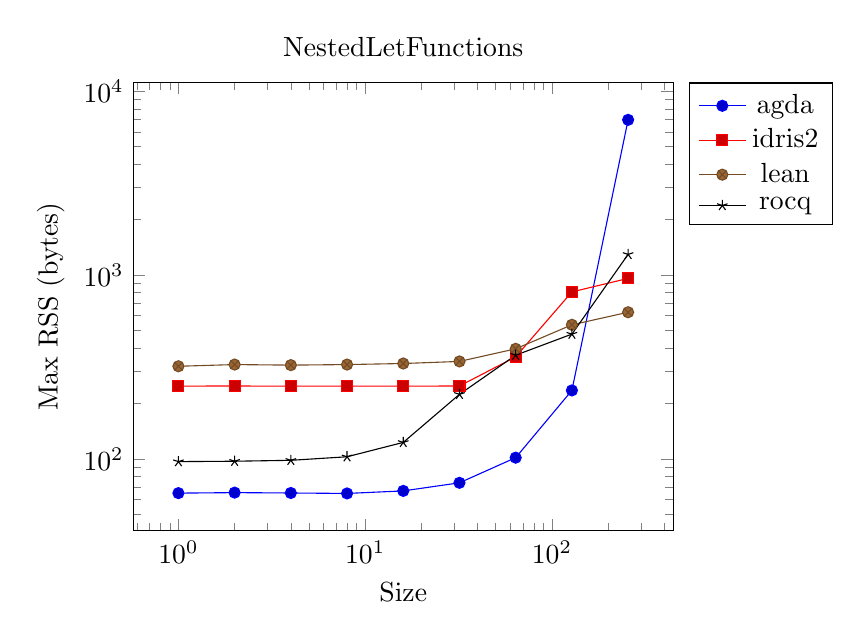
\begin{tikzpicture}
\begin{loglogaxis}
[title=NestedLetFunctions,
xlabel={Size},
ylabel={Max RSS (bytes)},
legend entries={agda,idris2,lean,rocq},
legend pos=outer north east,
]\addplot coordinates {
(256.0,6970.933248) [9]
(128.0,235.630592) [0]
(64.0,101.531648) [0]
(32.0,74.11712) [0]
(16.0,66.9696) [0]
(8.0,64.872448) [0]
(4.0,65.236992) [0]
(2.0,65.548288) [0]
(1.0,65.130496) [0]
};
\addplot coordinates {
(256.0,957.755392) [35072]
(128.0,808.771584) [35072]
(64.0,358.68672) [0]
(32.0,248.905728) [0]
(16.0,248.68864) [0]
(8.0,248.7296) [0]
(4.0,248.684544) [0]
(2.0,248.89344) [0]
(1.0,248.77056) [0]
};
\addplot coordinates {
(256.0,626.950144) [9]
(128.0,535.67488) [9]
(64.0,396.644352) [0]
(32.0,338.702336) [0]
(16.0,329.977856) [0]
(8.0,325.644288) [0]
(4.0,323.387392) [0]
(2.0,325.619712) [0]
(1.0,318.803968) [0]
};
\addplot coordinates {
(256.0,1293.410304) [0]
(128.0,476.749824) [0]
(64.0,366.256128) [0]
(32.0,224.354304) [0]
(16.0,122.884096) [0]
(8.0,102.670336) [0]
(4.0,98.213888) [0]
(2.0,97.087488) [0]
(1.0,96.620544) [0]
};
\end{loglogaxis}
\end{tikzpicture}


% \subsection{LargeIndexedParameterisedDatatype}
% 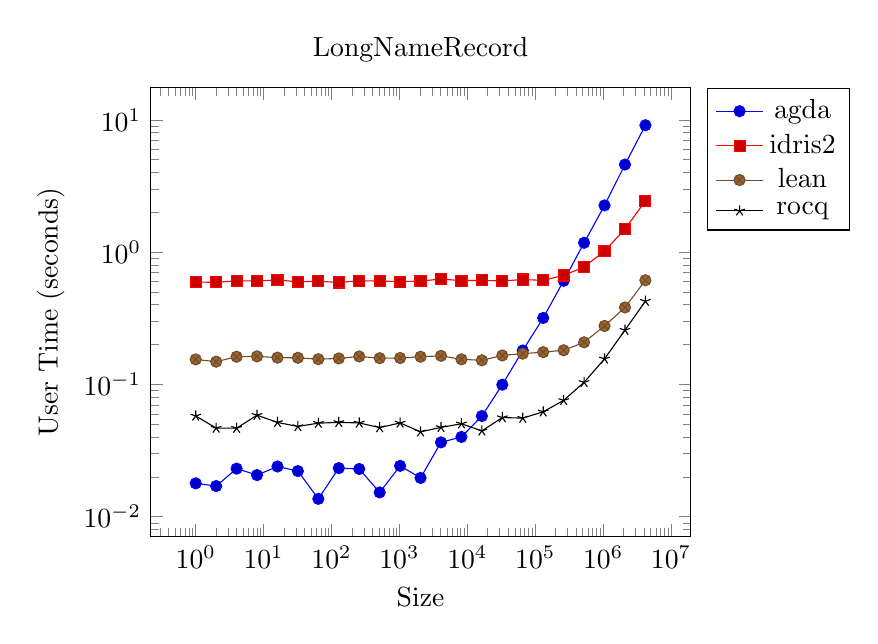
\begin{tikzpicture}
\begin{loglogaxis}
[title=LongNameRecord,
xlabel={Size},
ylabel={User Time (seconds)},
legend entries={agda,idris2,lean,rocq},
legend pos=outer north east,
]\addplot coordinates {
(4194304.0,9.097116) [0]
(2097152.0,4.588252) [0]
(1048576.0,2.253942) [0]
(524288.0,1.175644) [0]
(262144.0,0.606869) [0]
(131072.0,0.318102) [0]
(65536.0,0.180498) [0]
(32768.0,9.9566e-2) [0]
(16384.0,5.7703e-2) [0]
(8192.0,4.0103e-2) [0]
(4096.0,3.6509e-2) [0]
(2048.0,1.9649e-2) [0]
(1024.0,2.4239e-2) [0]
(512.0,1.5274e-2) [0]
(256.0,2.2951e-2) [0]
(128.0,2.3313e-2) [0]
(64.0,1.3655e-2) [0]
(32.0,2.2137e-2) [0]
(16.0,2.3973e-2) [0]
(8.0,2.0647e-2) [0]
(4.0,2.3102e-2) [0]
(2.0,1.7053e-2) [0]
(1.0,1.7885e-2) [0]
};
\addplot coordinates {
(4194304.0,2.435465) [0]
(2097152.0,1.494713) [0]
(1048576.0,1.018833) [0]
(524288.0,0.772144) [0]
(262144.0,0.66665) [0]
(131072.0,0.611889) [0]
(65536.0,0.620374) [0]
(32768.0,0.605496) [0]
(16384.0,0.611539) [0]
(8192.0,0.608788) [0]
(4096.0,0.626241) [0]
(2048.0,0.603874) [0]
(1024.0,0.598415) [0]
(512.0,0.604452) [0]
(256.0,0.60748) [0]
(128.0,0.589608) [0]
(64.0,0.603068) [0]
(32.0,0.596021) [0]
(16.0,0.616476) [0]
(8.0,0.605033) [0]
(4.0,0.606919) [0]
(2.0,0.591078) [0]
(1.0,0.594091) [0]
};
\addplot coordinates {
(4194304.0,0.612912) [0]
(2097152.0,0.381734) [0]
(1048576.0,0.276632) [0]
(524288.0,0.208152) [0]
(262144.0,0.181183) [0]
(131072.0,0.17531) [0]
(65536.0,0.170923) [0]
(32768.0,0.165527) [0]
(16384.0,0.15219) [0]
(8192.0,0.15478) [0]
(4096.0,0.164464) [0]
(2048.0,0.161915) [0]
(1024.0,0.158346) [0]
(512.0,0.157909) [0]
(256.0,0.162727) [0]
(128.0,0.157235) [0]
(64.0,0.155179) [0]
(32.0,0.158943) [0]
(16.0,0.159408) [0]
(8.0,0.162905) [0]
(4.0,0.16191) [0]
(2.0,0.148563) [0]
(1.0,0.15453) [0]
};
\addplot coordinates {
(4194304.0,0.426038) [0]
(2097152.0,0.257224) [0]
(1048576.0,0.156022) [0]
(524288.0,0.103696) [0]
(262144.0,7.5799e-2) [0]
(131072.0,6.2094e-2) [0]
(65536.0,5.5643e-2) [0]
(32768.0,5.6181e-2) [0]
(16384.0,4.4542e-2) [0]
(8192.0,5.0413e-2) [0]
(4096.0,4.7327e-2) [0]
(2048.0,4.3836e-2) [0]
(1024.0,5.1143e-2) [0]
(512.0,4.7186e-2) [0]
(256.0,5.1154e-2) [0]
(128.0,5.1667e-2) [0]
(64.0,5.0968e-2) [0]
(32.0,4.8123e-2) [0]
(16.0,5.1609e-2) [0]
(8.0,5.8562e-2) [0]
(4.0,4.6712e-2) [0]
(2.0,4.6796e-2) [0]
(1.0,5.7777e-2) [0]
};
\end{loglogaxis}
\end{tikzpicture}

% \\
% 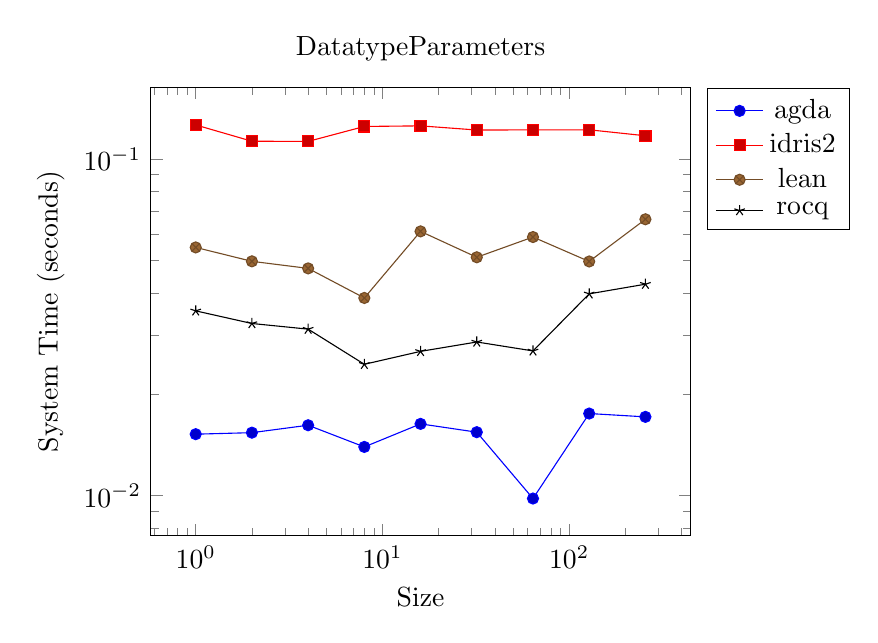
\begin{tikzpicture}
\begin{loglogaxis}
[title=DatatypeParameters,
xlabel={Size},
ylabel={System Time (seconds)},
legend entries={agda,idris2,lean,rocq},
legend pos=outer north east,
]\addplot coordinates {
(256.0,1.7155e-2) [0]
(128.0,1.755e-2) [0]
(64.0,9.813e-3) [0]
(32.0,1.545e-2) [0]
(16.0,1.6352e-2) [0]
(8.0,1.3967e-2) [0]
(4.0,1.62e-2) [0]
(2.0,1.5398e-2) [0]
(1.0,1.524e-2) [0]
};
\addplot coordinates {
(256.0,0.117316) [0]
(128.0,0.122186) [0]
(64.0,0.122117) [0]
(32.0,0.122001) [0]
(16.0,0.125521) [0]
(8.0,0.125017) [0]
(4.0,0.112862) [0]
(2.0,0.112996) [0]
(1.0,0.126323) [0]
};
\addplot coordinates {
(256.0,6.6273e-2) [256]
(128.0,4.9652e-2) [256]
(64.0,5.8684e-2) [0]
(32.0,5.1098e-2) [0]
(16.0,6.1002e-2) [0]
(8.0,3.8694e-2) [0]
(4.0,4.7356e-2) [0]
(2.0,4.9701e-2) [0]
(1.0,5.4661e-2) [0]
};
\addplot coordinates {
(256.0,4.2505e-2) [0]
(128.0,3.9801e-2) [0]
(64.0,2.6931e-2) [0]
(32.0,2.863e-2) [0]
(16.0,2.6848e-2) [0]
(8.0,2.4578e-2) [0]
(4.0,3.1258e-2) [0]
(2.0,3.2489e-2) [0]
(1.0,3.542e-2) [0]
};
\end{loglogaxis}
\end{tikzpicture}

% \\
% 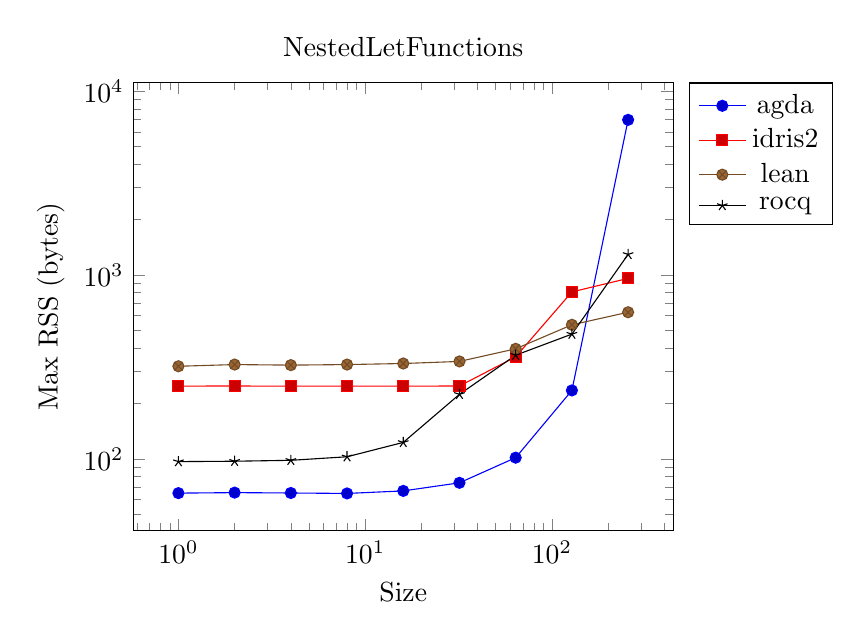
\begin{tikzpicture}
\begin{loglogaxis}
[title=NestedLetFunctions,
xlabel={Size},
ylabel={Max RSS (bytes)},
legend entries={agda,idris2,lean,rocq},
legend pos=outer north east,
]\addplot coordinates {
(256.0,6970.933248) [9]
(128.0,235.630592) [0]
(64.0,101.531648) [0]
(32.0,74.11712) [0]
(16.0,66.9696) [0]
(8.0,64.872448) [0]
(4.0,65.236992) [0]
(2.0,65.548288) [0]
(1.0,65.130496) [0]
};
\addplot coordinates {
(256.0,957.755392) [35072]
(128.0,808.771584) [35072]
(64.0,358.68672) [0]
(32.0,248.905728) [0]
(16.0,248.68864) [0]
(8.0,248.7296) [0]
(4.0,248.684544) [0]
(2.0,248.89344) [0]
(1.0,248.77056) [0]
};
\addplot coordinates {
(256.0,626.950144) [9]
(128.0,535.67488) [9]
(64.0,396.644352) [0]
(32.0,338.702336) [0]
(16.0,329.977856) [0]
(8.0,325.644288) [0]
(4.0,323.387392) [0]
(2.0,325.619712) [0]
(1.0,318.803968) [0]
};
\addplot coordinates {
(256.0,1293.410304) [0]
(128.0,476.749824) [0]
(64.0,366.256128) [0]
(32.0,224.354304) [0]
(16.0,122.884096) [0]
(8.0,102.670336) [0]
(4.0,98.213888) [0]
(2.0,97.087488) [0]
(1.0,96.620544) [0]
};
\end{loglogaxis}
\end{tikzpicture}


% \subsection{LargeLambda}
% 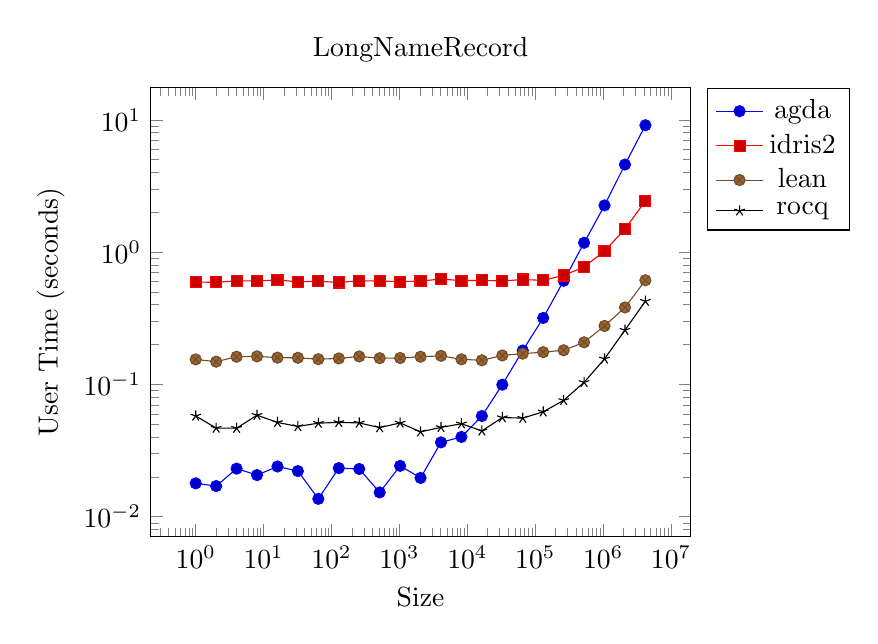
\begin{tikzpicture}
\begin{loglogaxis}
[title=LongNameRecord,
xlabel={Size},
ylabel={User Time (seconds)},
legend entries={agda,idris2,lean,rocq},
legend pos=outer north east,
]\addplot coordinates {
(4194304.0,9.097116) [0]
(2097152.0,4.588252) [0]
(1048576.0,2.253942) [0]
(524288.0,1.175644) [0]
(262144.0,0.606869) [0]
(131072.0,0.318102) [0]
(65536.0,0.180498) [0]
(32768.0,9.9566e-2) [0]
(16384.0,5.7703e-2) [0]
(8192.0,4.0103e-2) [0]
(4096.0,3.6509e-2) [0]
(2048.0,1.9649e-2) [0]
(1024.0,2.4239e-2) [0]
(512.0,1.5274e-2) [0]
(256.0,2.2951e-2) [0]
(128.0,2.3313e-2) [0]
(64.0,1.3655e-2) [0]
(32.0,2.2137e-2) [0]
(16.0,2.3973e-2) [0]
(8.0,2.0647e-2) [0]
(4.0,2.3102e-2) [0]
(2.0,1.7053e-2) [0]
(1.0,1.7885e-2) [0]
};
\addplot coordinates {
(4194304.0,2.435465) [0]
(2097152.0,1.494713) [0]
(1048576.0,1.018833) [0]
(524288.0,0.772144) [0]
(262144.0,0.66665) [0]
(131072.0,0.611889) [0]
(65536.0,0.620374) [0]
(32768.0,0.605496) [0]
(16384.0,0.611539) [0]
(8192.0,0.608788) [0]
(4096.0,0.626241) [0]
(2048.0,0.603874) [0]
(1024.0,0.598415) [0]
(512.0,0.604452) [0]
(256.0,0.60748) [0]
(128.0,0.589608) [0]
(64.0,0.603068) [0]
(32.0,0.596021) [0]
(16.0,0.616476) [0]
(8.0,0.605033) [0]
(4.0,0.606919) [0]
(2.0,0.591078) [0]
(1.0,0.594091) [0]
};
\addplot coordinates {
(4194304.0,0.612912) [0]
(2097152.0,0.381734) [0]
(1048576.0,0.276632) [0]
(524288.0,0.208152) [0]
(262144.0,0.181183) [0]
(131072.0,0.17531) [0]
(65536.0,0.170923) [0]
(32768.0,0.165527) [0]
(16384.0,0.15219) [0]
(8192.0,0.15478) [0]
(4096.0,0.164464) [0]
(2048.0,0.161915) [0]
(1024.0,0.158346) [0]
(512.0,0.157909) [0]
(256.0,0.162727) [0]
(128.0,0.157235) [0]
(64.0,0.155179) [0]
(32.0,0.158943) [0]
(16.0,0.159408) [0]
(8.0,0.162905) [0]
(4.0,0.16191) [0]
(2.0,0.148563) [0]
(1.0,0.15453) [0]
};
\addplot coordinates {
(4194304.0,0.426038) [0]
(2097152.0,0.257224) [0]
(1048576.0,0.156022) [0]
(524288.0,0.103696) [0]
(262144.0,7.5799e-2) [0]
(131072.0,6.2094e-2) [0]
(65536.0,5.5643e-2) [0]
(32768.0,5.6181e-2) [0]
(16384.0,4.4542e-2) [0]
(8192.0,5.0413e-2) [0]
(4096.0,4.7327e-2) [0]
(2048.0,4.3836e-2) [0]
(1024.0,5.1143e-2) [0]
(512.0,4.7186e-2) [0]
(256.0,5.1154e-2) [0]
(128.0,5.1667e-2) [0]
(64.0,5.0968e-2) [0]
(32.0,4.8123e-2) [0]
(16.0,5.1609e-2) [0]
(8.0,5.8562e-2) [0]
(4.0,4.6712e-2) [0]
(2.0,4.6796e-2) [0]
(1.0,5.7777e-2) [0]
};
\end{loglogaxis}
\end{tikzpicture}

% \\
% 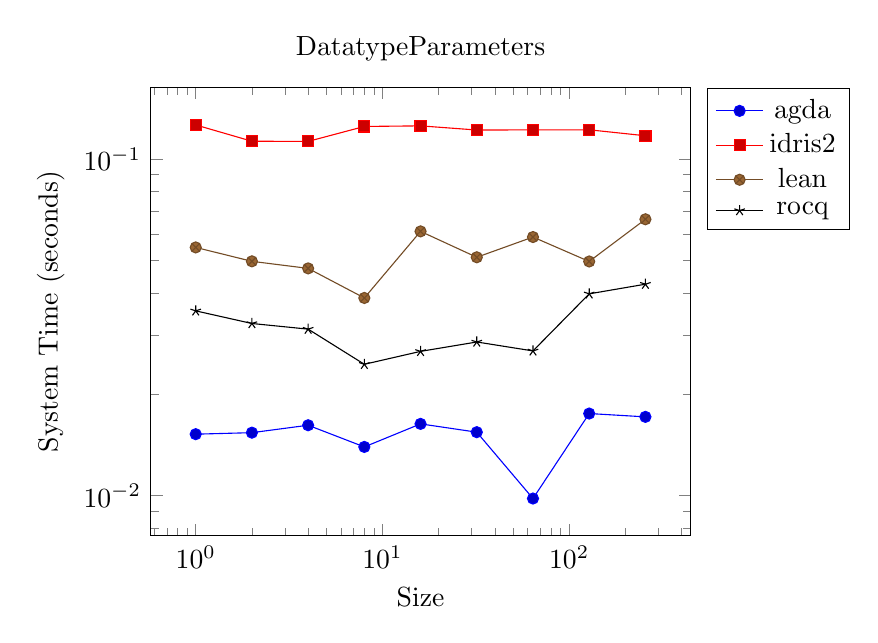
\begin{tikzpicture}
\begin{loglogaxis}
[title=DatatypeParameters,
xlabel={Size},
ylabel={System Time (seconds)},
legend entries={agda,idris2,lean,rocq},
legend pos=outer north east,
]\addplot coordinates {
(256.0,1.7155e-2) [0]
(128.0,1.755e-2) [0]
(64.0,9.813e-3) [0]
(32.0,1.545e-2) [0]
(16.0,1.6352e-2) [0]
(8.0,1.3967e-2) [0]
(4.0,1.62e-2) [0]
(2.0,1.5398e-2) [0]
(1.0,1.524e-2) [0]
};
\addplot coordinates {
(256.0,0.117316) [0]
(128.0,0.122186) [0]
(64.0,0.122117) [0]
(32.0,0.122001) [0]
(16.0,0.125521) [0]
(8.0,0.125017) [0]
(4.0,0.112862) [0]
(2.0,0.112996) [0]
(1.0,0.126323) [0]
};
\addplot coordinates {
(256.0,6.6273e-2) [256]
(128.0,4.9652e-2) [256]
(64.0,5.8684e-2) [0]
(32.0,5.1098e-2) [0]
(16.0,6.1002e-2) [0]
(8.0,3.8694e-2) [0]
(4.0,4.7356e-2) [0]
(2.0,4.9701e-2) [0]
(1.0,5.4661e-2) [0]
};
\addplot coordinates {
(256.0,4.2505e-2) [0]
(128.0,3.9801e-2) [0]
(64.0,2.6931e-2) [0]
(32.0,2.863e-2) [0]
(16.0,2.6848e-2) [0]
(8.0,2.4578e-2) [0]
(4.0,3.1258e-2) [0]
(2.0,3.2489e-2) [0]
(1.0,3.542e-2) [0]
};
\end{loglogaxis}
\end{tikzpicture}

% \\
% 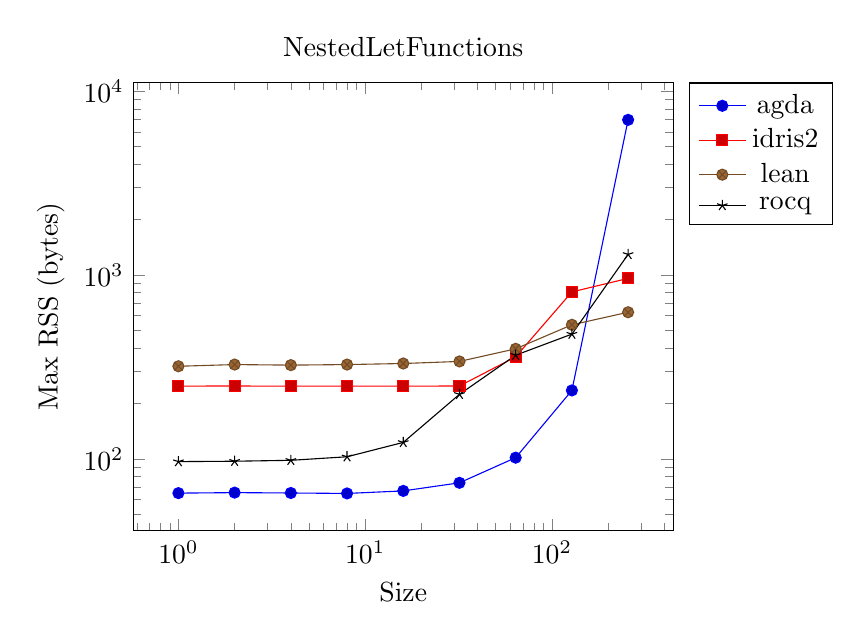
\begin{tikzpicture}
\begin{loglogaxis}
[title=NestedLetFunctions,
xlabel={Size},
ylabel={Max RSS (bytes)},
legend entries={agda,idris2,lean,rocq},
legend pos=outer north east,
]\addplot coordinates {
(256.0,6970.933248) [9]
(128.0,235.630592) [0]
(64.0,101.531648) [0]
(32.0,74.11712) [0]
(16.0,66.9696) [0]
(8.0,64.872448) [0]
(4.0,65.236992) [0]
(2.0,65.548288) [0]
(1.0,65.130496) [0]
};
\addplot coordinates {
(256.0,957.755392) [35072]
(128.0,808.771584) [35072]
(64.0,358.68672) [0]
(32.0,248.905728) [0]
(16.0,248.68864) [0]
(8.0,248.7296) [0]
(4.0,248.684544) [0]
(2.0,248.89344) [0]
(1.0,248.77056) [0]
};
\addplot coordinates {
(256.0,626.950144) [9]
(128.0,535.67488) [9]
(64.0,396.644352) [0]
(32.0,338.702336) [0]
(16.0,329.977856) [0]
(8.0,325.644288) [0]
(4.0,323.387392) [0]
(2.0,325.619712) [0]
(1.0,318.803968) [0]
};
\addplot coordinates {
(256.0,1293.410304) [0]
(128.0,476.749824) [0]
(64.0,366.256128) [0]
(32.0,224.354304) [0]
(16.0,122.884096) [0]
(8.0,102.670336) [0]
(4.0,98.213888) [0]
(2.0,97.087488) [0]
(1.0,96.620544) [0]
};
\end{loglogaxis}
\end{tikzpicture}


% \subsection{LargeSimpleDatatype}
% 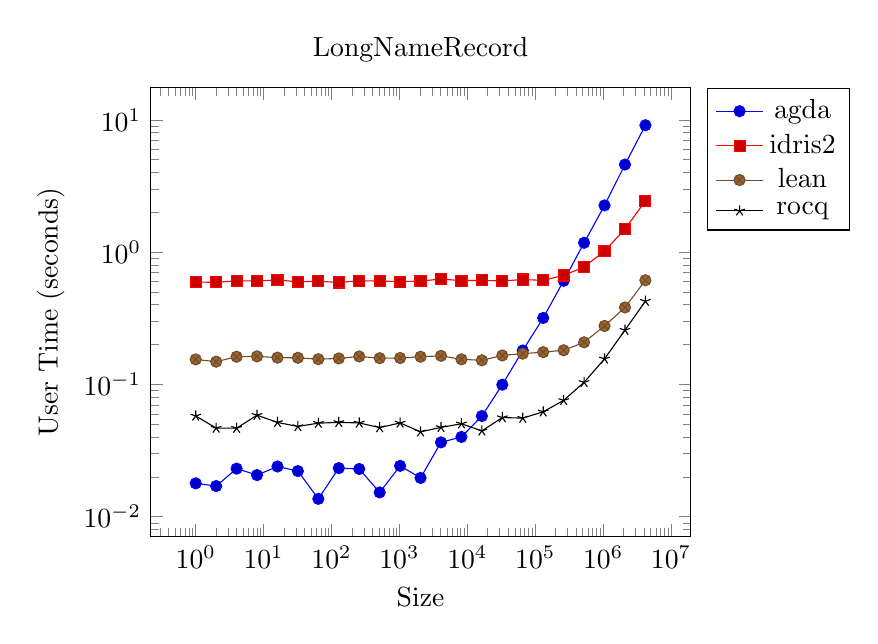
\begin{tikzpicture}
\begin{loglogaxis}
[title=LongNameRecord,
xlabel={Size},
ylabel={User Time (seconds)},
legend entries={agda,idris2,lean,rocq},
legend pos=outer north east,
]\addplot coordinates {
(4194304.0,9.097116) [0]
(2097152.0,4.588252) [0]
(1048576.0,2.253942) [0]
(524288.0,1.175644) [0]
(262144.0,0.606869) [0]
(131072.0,0.318102) [0]
(65536.0,0.180498) [0]
(32768.0,9.9566e-2) [0]
(16384.0,5.7703e-2) [0]
(8192.0,4.0103e-2) [0]
(4096.0,3.6509e-2) [0]
(2048.0,1.9649e-2) [0]
(1024.0,2.4239e-2) [0]
(512.0,1.5274e-2) [0]
(256.0,2.2951e-2) [0]
(128.0,2.3313e-2) [0]
(64.0,1.3655e-2) [0]
(32.0,2.2137e-2) [0]
(16.0,2.3973e-2) [0]
(8.0,2.0647e-2) [0]
(4.0,2.3102e-2) [0]
(2.0,1.7053e-2) [0]
(1.0,1.7885e-2) [0]
};
\addplot coordinates {
(4194304.0,2.435465) [0]
(2097152.0,1.494713) [0]
(1048576.0,1.018833) [0]
(524288.0,0.772144) [0]
(262144.0,0.66665) [0]
(131072.0,0.611889) [0]
(65536.0,0.620374) [0]
(32768.0,0.605496) [0]
(16384.0,0.611539) [0]
(8192.0,0.608788) [0]
(4096.0,0.626241) [0]
(2048.0,0.603874) [0]
(1024.0,0.598415) [0]
(512.0,0.604452) [0]
(256.0,0.60748) [0]
(128.0,0.589608) [0]
(64.0,0.603068) [0]
(32.0,0.596021) [0]
(16.0,0.616476) [0]
(8.0,0.605033) [0]
(4.0,0.606919) [0]
(2.0,0.591078) [0]
(1.0,0.594091) [0]
};
\addplot coordinates {
(4194304.0,0.612912) [0]
(2097152.0,0.381734) [0]
(1048576.0,0.276632) [0]
(524288.0,0.208152) [0]
(262144.0,0.181183) [0]
(131072.0,0.17531) [0]
(65536.0,0.170923) [0]
(32768.0,0.165527) [0]
(16384.0,0.15219) [0]
(8192.0,0.15478) [0]
(4096.0,0.164464) [0]
(2048.0,0.161915) [0]
(1024.0,0.158346) [0]
(512.0,0.157909) [0]
(256.0,0.162727) [0]
(128.0,0.157235) [0]
(64.0,0.155179) [0]
(32.0,0.158943) [0]
(16.0,0.159408) [0]
(8.0,0.162905) [0]
(4.0,0.16191) [0]
(2.0,0.148563) [0]
(1.0,0.15453) [0]
};
\addplot coordinates {
(4194304.0,0.426038) [0]
(2097152.0,0.257224) [0]
(1048576.0,0.156022) [0]
(524288.0,0.103696) [0]
(262144.0,7.5799e-2) [0]
(131072.0,6.2094e-2) [0]
(65536.0,5.5643e-2) [0]
(32768.0,5.6181e-2) [0]
(16384.0,4.4542e-2) [0]
(8192.0,5.0413e-2) [0]
(4096.0,4.7327e-2) [0]
(2048.0,4.3836e-2) [0]
(1024.0,5.1143e-2) [0]
(512.0,4.7186e-2) [0]
(256.0,5.1154e-2) [0]
(128.0,5.1667e-2) [0]
(64.0,5.0968e-2) [0]
(32.0,4.8123e-2) [0]
(16.0,5.1609e-2) [0]
(8.0,5.8562e-2) [0]
(4.0,4.6712e-2) [0]
(2.0,4.6796e-2) [0]
(1.0,5.7777e-2) [0]
};
\end{loglogaxis}
\end{tikzpicture}

% \\
% 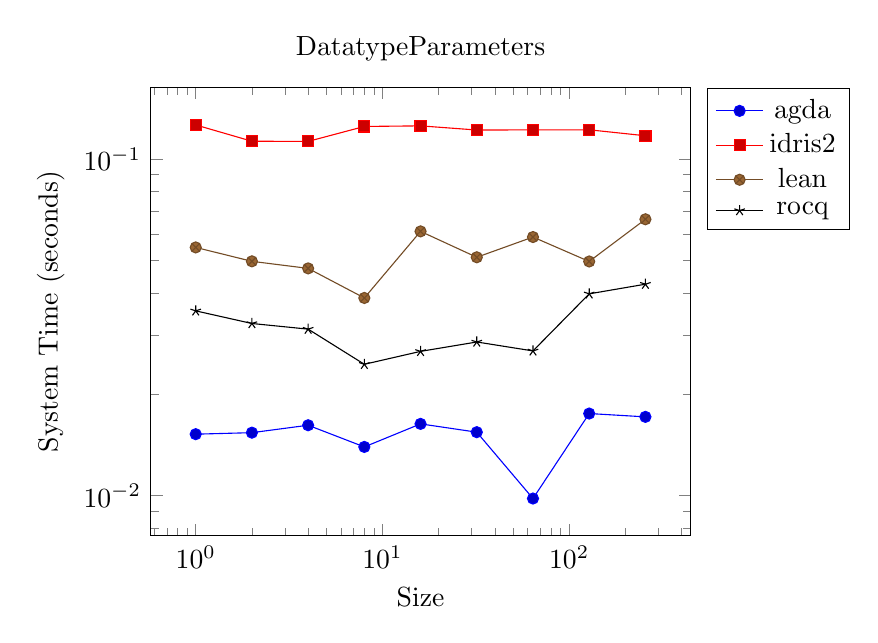
\begin{tikzpicture}
\begin{loglogaxis}
[title=DatatypeParameters,
xlabel={Size},
ylabel={System Time (seconds)},
legend entries={agda,idris2,lean,rocq},
legend pos=outer north east,
]\addplot coordinates {
(256.0,1.7155e-2) [0]
(128.0,1.755e-2) [0]
(64.0,9.813e-3) [0]
(32.0,1.545e-2) [0]
(16.0,1.6352e-2) [0]
(8.0,1.3967e-2) [0]
(4.0,1.62e-2) [0]
(2.0,1.5398e-2) [0]
(1.0,1.524e-2) [0]
};
\addplot coordinates {
(256.0,0.117316) [0]
(128.0,0.122186) [0]
(64.0,0.122117) [0]
(32.0,0.122001) [0]
(16.0,0.125521) [0]
(8.0,0.125017) [0]
(4.0,0.112862) [0]
(2.0,0.112996) [0]
(1.0,0.126323) [0]
};
\addplot coordinates {
(256.0,6.6273e-2) [256]
(128.0,4.9652e-2) [256]
(64.0,5.8684e-2) [0]
(32.0,5.1098e-2) [0]
(16.0,6.1002e-2) [0]
(8.0,3.8694e-2) [0]
(4.0,4.7356e-2) [0]
(2.0,4.9701e-2) [0]
(1.0,5.4661e-2) [0]
};
\addplot coordinates {
(256.0,4.2505e-2) [0]
(128.0,3.9801e-2) [0]
(64.0,2.6931e-2) [0]
(32.0,2.863e-2) [0]
(16.0,2.6848e-2) [0]
(8.0,2.4578e-2) [0]
(4.0,3.1258e-2) [0]
(2.0,3.2489e-2) [0]
(1.0,3.542e-2) [0]
};
\end{loglogaxis}
\end{tikzpicture}

% \\
% 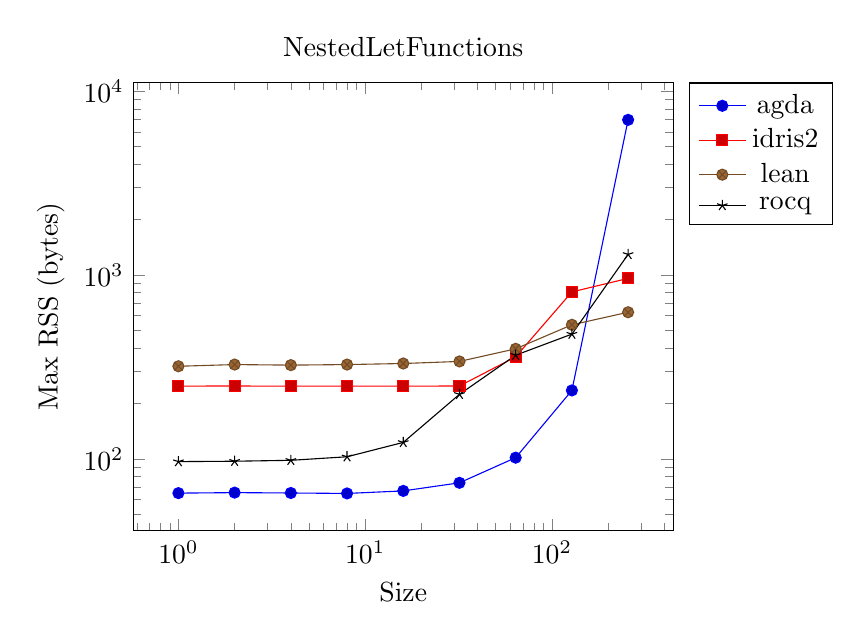
\begin{tikzpicture}
\begin{loglogaxis}
[title=NestedLetFunctions,
xlabel={Size},
ylabel={Max RSS (bytes)},
legend entries={agda,idris2,lean,rocq},
legend pos=outer north east,
]\addplot coordinates {
(256.0,6970.933248) [9]
(128.0,235.630592) [0]
(64.0,101.531648) [0]
(32.0,74.11712) [0]
(16.0,66.9696) [0]
(8.0,64.872448) [0]
(4.0,65.236992) [0]
(2.0,65.548288) [0]
(1.0,65.130496) [0]
};
\addplot coordinates {
(256.0,957.755392) [35072]
(128.0,808.771584) [35072]
(64.0,358.68672) [0]
(32.0,248.905728) [0]
(16.0,248.68864) [0]
(8.0,248.7296) [0]
(4.0,248.684544) [0]
(2.0,248.89344) [0]
(1.0,248.77056) [0]
};
\addplot coordinates {
(256.0,626.950144) [9]
(128.0,535.67488) [9]
(64.0,396.644352) [0]
(32.0,338.702336) [0]
(16.0,329.977856) [0]
(8.0,325.644288) [0]
(4.0,323.387392) [0]
(2.0,325.619712) [0]
(1.0,318.803968) [0]
};
\addplot coordinates {
(256.0,1293.410304) [0]
(128.0,476.749824) [0]
(64.0,366.256128) [0]
(32.0,224.354304) [0]
(16.0,122.884096) [0]
(8.0,102.670336) [0]
(4.0,98.213888) [0]
(2.0,97.087488) [0]
(1.0,96.620544) [0]
};
\end{loglogaxis}
\end{tikzpicture}


% \subsection{LargeSimpleRecord}
% 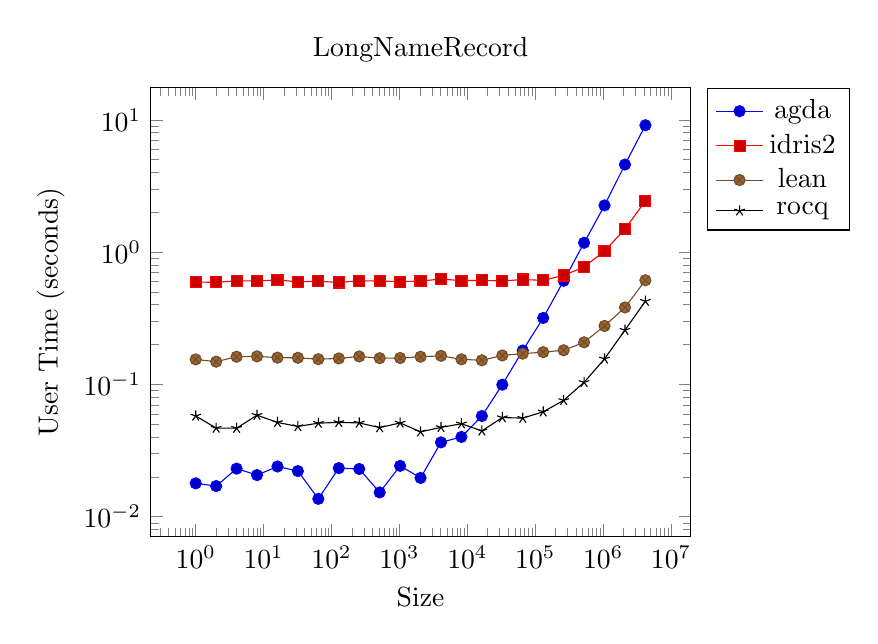
\begin{tikzpicture}
\begin{loglogaxis}
[title=LongNameRecord,
xlabel={Size},
ylabel={User Time (seconds)},
legend entries={agda,idris2,lean,rocq},
legend pos=outer north east,
]\addplot coordinates {
(4194304.0,9.097116) [0]
(2097152.0,4.588252) [0]
(1048576.0,2.253942) [0]
(524288.0,1.175644) [0]
(262144.0,0.606869) [0]
(131072.0,0.318102) [0]
(65536.0,0.180498) [0]
(32768.0,9.9566e-2) [0]
(16384.0,5.7703e-2) [0]
(8192.0,4.0103e-2) [0]
(4096.0,3.6509e-2) [0]
(2048.0,1.9649e-2) [0]
(1024.0,2.4239e-2) [0]
(512.0,1.5274e-2) [0]
(256.0,2.2951e-2) [0]
(128.0,2.3313e-2) [0]
(64.0,1.3655e-2) [0]
(32.0,2.2137e-2) [0]
(16.0,2.3973e-2) [0]
(8.0,2.0647e-2) [0]
(4.0,2.3102e-2) [0]
(2.0,1.7053e-2) [0]
(1.0,1.7885e-2) [0]
};
\addplot coordinates {
(4194304.0,2.435465) [0]
(2097152.0,1.494713) [0]
(1048576.0,1.018833) [0]
(524288.0,0.772144) [0]
(262144.0,0.66665) [0]
(131072.0,0.611889) [0]
(65536.0,0.620374) [0]
(32768.0,0.605496) [0]
(16384.0,0.611539) [0]
(8192.0,0.608788) [0]
(4096.0,0.626241) [0]
(2048.0,0.603874) [0]
(1024.0,0.598415) [0]
(512.0,0.604452) [0]
(256.0,0.60748) [0]
(128.0,0.589608) [0]
(64.0,0.603068) [0]
(32.0,0.596021) [0]
(16.0,0.616476) [0]
(8.0,0.605033) [0]
(4.0,0.606919) [0]
(2.0,0.591078) [0]
(1.0,0.594091) [0]
};
\addplot coordinates {
(4194304.0,0.612912) [0]
(2097152.0,0.381734) [0]
(1048576.0,0.276632) [0]
(524288.0,0.208152) [0]
(262144.0,0.181183) [0]
(131072.0,0.17531) [0]
(65536.0,0.170923) [0]
(32768.0,0.165527) [0]
(16384.0,0.15219) [0]
(8192.0,0.15478) [0]
(4096.0,0.164464) [0]
(2048.0,0.161915) [0]
(1024.0,0.158346) [0]
(512.0,0.157909) [0]
(256.0,0.162727) [0]
(128.0,0.157235) [0]
(64.0,0.155179) [0]
(32.0,0.158943) [0]
(16.0,0.159408) [0]
(8.0,0.162905) [0]
(4.0,0.16191) [0]
(2.0,0.148563) [0]
(1.0,0.15453) [0]
};
\addplot coordinates {
(4194304.0,0.426038) [0]
(2097152.0,0.257224) [0]
(1048576.0,0.156022) [0]
(524288.0,0.103696) [0]
(262144.0,7.5799e-2) [0]
(131072.0,6.2094e-2) [0]
(65536.0,5.5643e-2) [0]
(32768.0,5.6181e-2) [0]
(16384.0,4.4542e-2) [0]
(8192.0,5.0413e-2) [0]
(4096.0,4.7327e-2) [0]
(2048.0,4.3836e-2) [0]
(1024.0,5.1143e-2) [0]
(512.0,4.7186e-2) [0]
(256.0,5.1154e-2) [0]
(128.0,5.1667e-2) [0]
(64.0,5.0968e-2) [0]
(32.0,4.8123e-2) [0]
(16.0,5.1609e-2) [0]
(8.0,5.8562e-2) [0]
(4.0,4.6712e-2) [0]
(2.0,4.6796e-2) [0]
(1.0,5.7777e-2) [0]
};
\end{loglogaxis}
\end{tikzpicture}

% \\
% 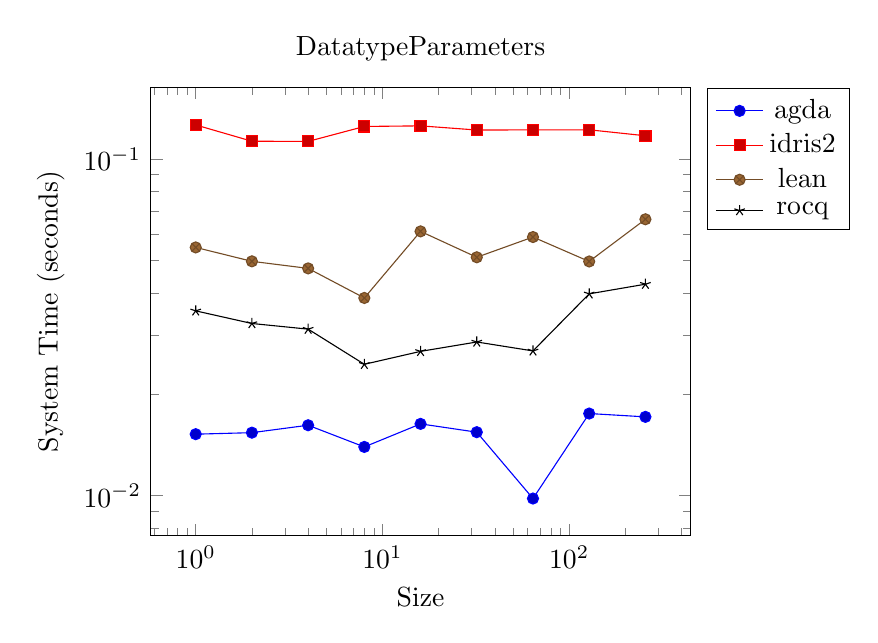
\begin{tikzpicture}
\begin{loglogaxis}
[title=DatatypeParameters,
xlabel={Size},
ylabel={System Time (seconds)},
legend entries={agda,idris2,lean,rocq},
legend pos=outer north east,
]\addplot coordinates {
(256.0,1.7155e-2) [0]
(128.0,1.755e-2) [0]
(64.0,9.813e-3) [0]
(32.0,1.545e-2) [0]
(16.0,1.6352e-2) [0]
(8.0,1.3967e-2) [0]
(4.0,1.62e-2) [0]
(2.0,1.5398e-2) [0]
(1.0,1.524e-2) [0]
};
\addplot coordinates {
(256.0,0.117316) [0]
(128.0,0.122186) [0]
(64.0,0.122117) [0]
(32.0,0.122001) [0]
(16.0,0.125521) [0]
(8.0,0.125017) [0]
(4.0,0.112862) [0]
(2.0,0.112996) [0]
(1.0,0.126323) [0]
};
\addplot coordinates {
(256.0,6.6273e-2) [256]
(128.0,4.9652e-2) [256]
(64.0,5.8684e-2) [0]
(32.0,5.1098e-2) [0]
(16.0,6.1002e-2) [0]
(8.0,3.8694e-2) [0]
(4.0,4.7356e-2) [0]
(2.0,4.9701e-2) [0]
(1.0,5.4661e-2) [0]
};
\addplot coordinates {
(256.0,4.2505e-2) [0]
(128.0,3.9801e-2) [0]
(64.0,2.6931e-2) [0]
(32.0,2.863e-2) [0]
(16.0,2.6848e-2) [0]
(8.0,2.4578e-2) [0]
(4.0,3.1258e-2) [0]
(2.0,3.2489e-2) [0]
(1.0,3.542e-2) [0]
};
\end{loglogaxis}
\end{tikzpicture}

% \\
% 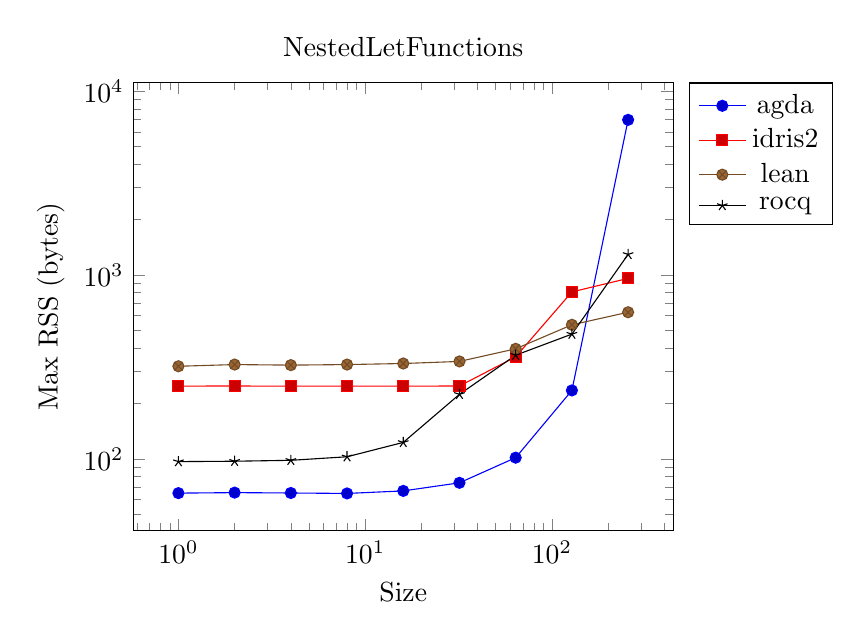
\begin{tikzpicture}
\begin{loglogaxis}
[title=NestedLetFunctions,
xlabel={Size},
ylabel={Max RSS (bytes)},
legend entries={agda,idris2,lean,rocq},
legend pos=outer north east,
]\addplot coordinates {
(256.0,6970.933248) [9]
(128.0,235.630592) [0]
(64.0,101.531648) [0]
(32.0,74.11712) [0]
(16.0,66.9696) [0]
(8.0,64.872448) [0]
(4.0,65.236992) [0]
(2.0,65.548288) [0]
(1.0,65.130496) [0]
};
\addplot coordinates {
(256.0,957.755392) [35072]
(128.0,808.771584) [35072]
(64.0,358.68672) [0]
(32.0,248.905728) [0]
(16.0,248.68864) [0]
(8.0,248.7296) [0]
(4.0,248.684544) [0]
(2.0,248.89344) [0]
(1.0,248.77056) [0]
};
\addplot coordinates {
(256.0,626.950144) [9]
(128.0,535.67488) [9]
(64.0,396.644352) [0]
(32.0,338.702336) [0]
(16.0,329.977856) [0]
(8.0,325.644288) [0]
(4.0,323.387392) [0]
(2.0,325.619712) [0]
(1.0,318.803968) [0]
};
\addplot coordinates {
(256.0,1293.410304) [0]
(128.0,476.749824) [0]
(64.0,366.256128) [0]
(32.0,224.354304) [0]
(16.0,122.884096) [0]
(8.0,102.670336) [0]
(4.0,98.213888) [0]
(2.0,97.087488) [0]
(1.0,96.620544) [0]
};
\end{loglogaxis}
\end{tikzpicture}


% \subsection{LongNameDatatype}
% 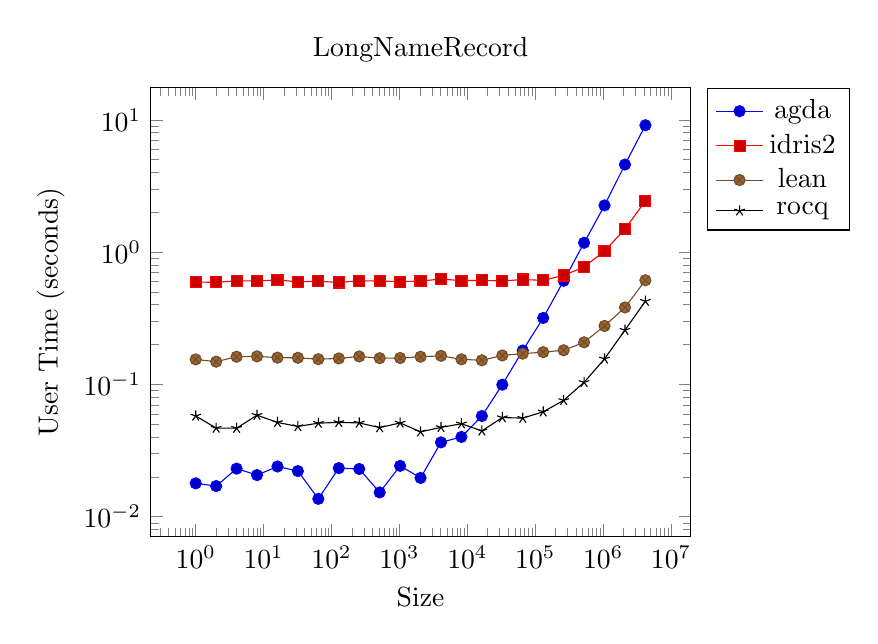
\begin{tikzpicture}
\begin{loglogaxis}
[title=LongNameRecord,
xlabel={Size},
ylabel={User Time (seconds)},
legend entries={agda,idris2,lean,rocq},
legend pos=outer north east,
]\addplot coordinates {
(4194304.0,9.097116) [0]
(2097152.0,4.588252) [0]
(1048576.0,2.253942) [0]
(524288.0,1.175644) [0]
(262144.0,0.606869) [0]
(131072.0,0.318102) [0]
(65536.0,0.180498) [0]
(32768.0,9.9566e-2) [0]
(16384.0,5.7703e-2) [0]
(8192.0,4.0103e-2) [0]
(4096.0,3.6509e-2) [0]
(2048.0,1.9649e-2) [0]
(1024.0,2.4239e-2) [0]
(512.0,1.5274e-2) [0]
(256.0,2.2951e-2) [0]
(128.0,2.3313e-2) [0]
(64.0,1.3655e-2) [0]
(32.0,2.2137e-2) [0]
(16.0,2.3973e-2) [0]
(8.0,2.0647e-2) [0]
(4.0,2.3102e-2) [0]
(2.0,1.7053e-2) [0]
(1.0,1.7885e-2) [0]
};
\addplot coordinates {
(4194304.0,2.435465) [0]
(2097152.0,1.494713) [0]
(1048576.0,1.018833) [0]
(524288.0,0.772144) [0]
(262144.0,0.66665) [0]
(131072.0,0.611889) [0]
(65536.0,0.620374) [0]
(32768.0,0.605496) [0]
(16384.0,0.611539) [0]
(8192.0,0.608788) [0]
(4096.0,0.626241) [0]
(2048.0,0.603874) [0]
(1024.0,0.598415) [0]
(512.0,0.604452) [0]
(256.0,0.60748) [0]
(128.0,0.589608) [0]
(64.0,0.603068) [0]
(32.0,0.596021) [0]
(16.0,0.616476) [0]
(8.0,0.605033) [0]
(4.0,0.606919) [0]
(2.0,0.591078) [0]
(1.0,0.594091) [0]
};
\addplot coordinates {
(4194304.0,0.612912) [0]
(2097152.0,0.381734) [0]
(1048576.0,0.276632) [0]
(524288.0,0.208152) [0]
(262144.0,0.181183) [0]
(131072.0,0.17531) [0]
(65536.0,0.170923) [0]
(32768.0,0.165527) [0]
(16384.0,0.15219) [0]
(8192.0,0.15478) [0]
(4096.0,0.164464) [0]
(2048.0,0.161915) [0]
(1024.0,0.158346) [0]
(512.0,0.157909) [0]
(256.0,0.162727) [0]
(128.0,0.157235) [0]
(64.0,0.155179) [0]
(32.0,0.158943) [0]
(16.0,0.159408) [0]
(8.0,0.162905) [0]
(4.0,0.16191) [0]
(2.0,0.148563) [0]
(1.0,0.15453) [0]
};
\addplot coordinates {
(4194304.0,0.426038) [0]
(2097152.0,0.257224) [0]
(1048576.0,0.156022) [0]
(524288.0,0.103696) [0]
(262144.0,7.5799e-2) [0]
(131072.0,6.2094e-2) [0]
(65536.0,5.5643e-2) [0]
(32768.0,5.6181e-2) [0]
(16384.0,4.4542e-2) [0]
(8192.0,5.0413e-2) [0]
(4096.0,4.7327e-2) [0]
(2048.0,4.3836e-2) [0]
(1024.0,5.1143e-2) [0]
(512.0,4.7186e-2) [0]
(256.0,5.1154e-2) [0]
(128.0,5.1667e-2) [0]
(64.0,5.0968e-2) [0]
(32.0,4.8123e-2) [0]
(16.0,5.1609e-2) [0]
(8.0,5.8562e-2) [0]
(4.0,4.6712e-2) [0]
(2.0,4.6796e-2) [0]
(1.0,5.7777e-2) [0]
};
\end{loglogaxis}
\end{tikzpicture}

% \\
% 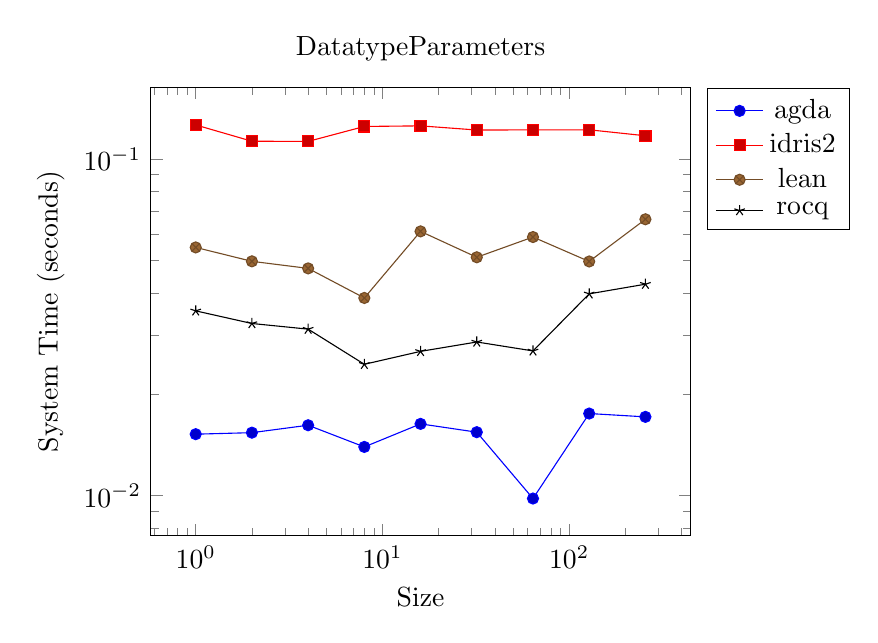
\begin{tikzpicture}
\begin{loglogaxis}
[title=DatatypeParameters,
xlabel={Size},
ylabel={System Time (seconds)},
legend entries={agda,idris2,lean,rocq},
legend pos=outer north east,
]\addplot coordinates {
(256.0,1.7155e-2) [0]
(128.0,1.755e-2) [0]
(64.0,9.813e-3) [0]
(32.0,1.545e-2) [0]
(16.0,1.6352e-2) [0]
(8.0,1.3967e-2) [0]
(4.0,1.62e-2) [0]
(2.0,1.5398e-2) [0]
(1.0,1.524e-2) [0]
};
\addplot coordinates {
(256.0,0.117316) [0]
(128.0,0.122186) [0]
(64.0,0.122117) [0]
(32.0,0.122001) [0]
(16.0,0.125521) [0]
(8.0,0.125017) [0]
(4.0,0.112862) [0]
(2.0,0.112996) [0]
(1.0,0.126323) [0]
};
\addplot coordinates {
(256.0,6.6273e-2) [256]
(128.0,4.9652e-2) [256]
(64.0,5.8684e-2) [0]
(32.0,5.1098e-2) [0]
(16.0,6.1002e-2) [0]
(8.0,3.8694e-2) [0]
(4.0,4.7356e-2) [0]
(2.0,4.9701e-2) [0]
(1.0,5.4661e-2) [0]
};
\addplot coordinates {
(256.0,4.2505e-2) [0]
(128.0,3.9801e-2) [0]
(64.0,2.6931e-2) [0]
(32.0,2.863e-2) [0]
(16.0,2.6848e-2) [0]
(8.0,2.4578e-2) [0]
(4.0,3.1258e-2) [0]
(2.0,3.2489e-2) [0]
(1.0,3.542e-2) [0]
};
\end{loglogaxis}
\end{tikzpicture}

% \\
% 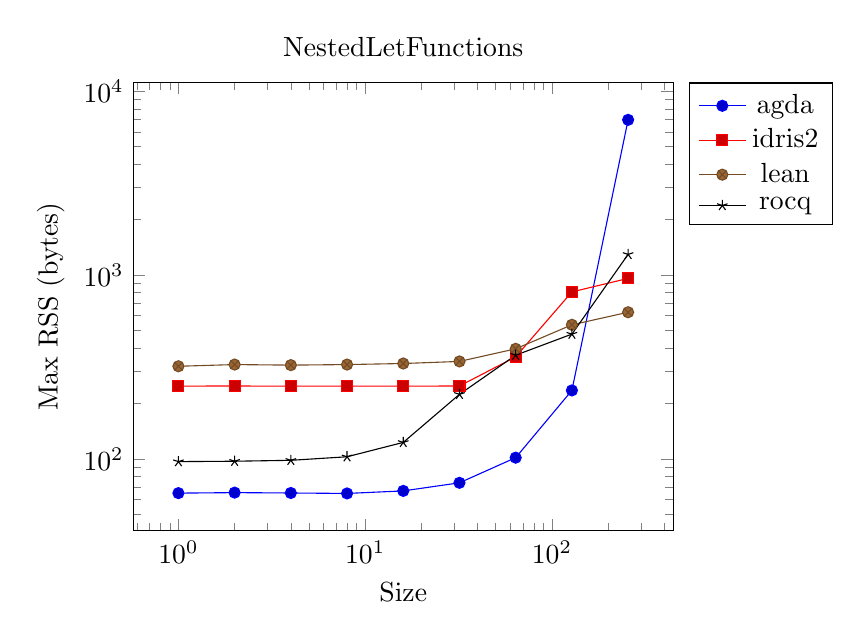
\begin{tikzpicture}
\begin{loglogaxis}
[title=NestedLetFunctions,
xlabel={Size},
ylabel={Max RSS (bytes)},
legend entries={agda,idris2,lean,rocq},
legend pos=outer north east,
]\addplot coordinates {
(256.0,6970.933248) [9]
(128.0,235.630592) [0]
(64.0,101.531648) [0]
(32.0,74.11712) [0]
(16.0,66.9696) [0]
(8.0,64.872448) [0]
(4.0,65.236992) [0]
(2.0,65.548288) [0]
(1.0,65.130496) [0]
};
\addplot coordinates {
(256.0,957.755392) [35072]
(128.0,808.771584) [35072]
(64.0,358.68672) [0]
(32.0,248.905728) [0]
(16.0,248.68864) [0]
(8.0,248.7296) [0]
(4.0,248.684544) [0]
(2.0,248.89344) [0]
(1.0,248.77056) [0]
};
\addplot coordinates {
(256.0,626.950144) [9]
(128.0,535.67488) [9]
(64.0,396.644352) [0]
(32.0,338.702336) [0]
(16.0,329.977856) [0]
(8.0,325.644288) [0]
(4.0,323.387392) [0]
(2.0,325.619712) [0]
(1.0,318.803968) [0]
};
\addplot coordinates {
(256.0,1293.410304) [0]
(128.0,476.749824) [0]
(64.0,366.256128) [0]
(32.0,224.354304) [0]
(16.0,122.884096) [0]
(8.0,102.670336) [0]
(4.0,98.213888) [0]
(2.0,97.087488) [0]
(1.0,96.620544) [0]
};
\end{loglogaxis}
\end{tikzpicture}


% \subsection{LongNameDatatypeConstructor}
% 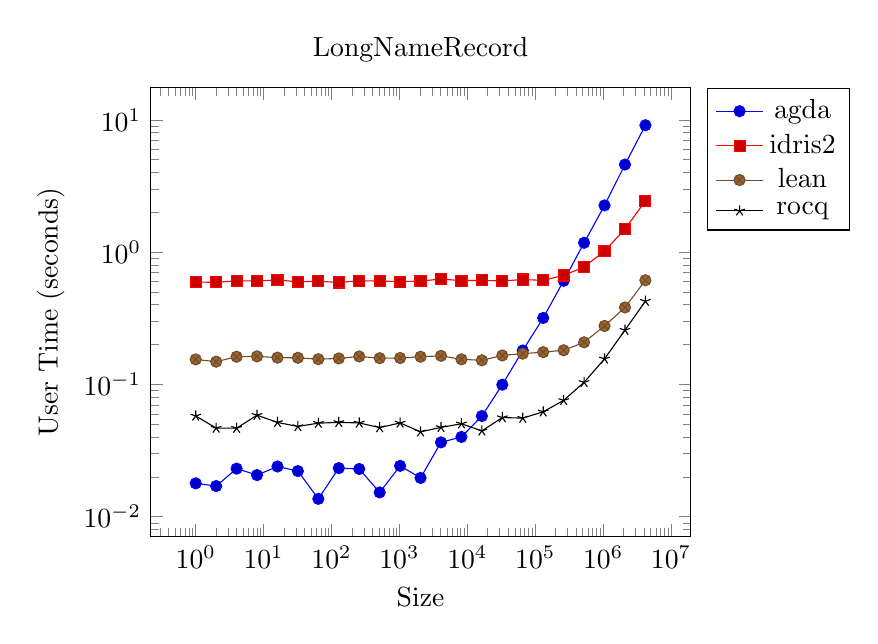
\begin{tikzpicture}
\begin{loglogaxis}
[title=LongNameRecord,
xlabel={Size},
ylabel={User Time (seconds)},
legend entries={agda,idris2,lean,rocq},
legend pos=outer north east,
]\addplot coordinates {
(4194304.0,9.097116) [0]
(2097152.0,4.588252) [0]
(1048576.0,2.253942) [0]
(524288.0,1.175644) [0]
(262144.0,0.606869) [0]
(131072.0,0.318102) [0]
(65536.0,0.180498) [0]
(32768.0,9.9566e-2) [0]
(16384.0,5.7703e-2) [0]
(8192.0,4.0103e-2) [0]
(4096.0,3.6509e-2) [0]
(2048.0,1.9649e-2) [0]
(1024.0,2.4239e-2) [0]
(512.0,1.5274e-2) [0]
(256.0,2.2951e-2) [0]
(128.0,2.3313e-2) [0]
(64.0,1.3655e-2) [0]
(32.0,2.2137e-2) [0]
(16.0,2.3973e-2) [0]
(8.0,2.0647e-2) [0]
(4.0,2.3102e-2) [0]
(2.0,1.7053e-2) [0]
(1.0,1.7885e-2) [0]
};
\addplot coordinates {
(4194304.0,2.435465) [0]
(2097152.0,1.494713) [0]
(1048576.0,1.018833) [0]
(524288.0,0.772144) [0]
(262144.0,0.66665) [0]
(131072.0,0.611889) [0]
(65536.0,0.620374) [0]
(32768.0,0.605496) [0]
(16384.0,0.611539) [0]
(8192.0,0.608788) [0]
(4096.0,0.626241) [0]
(2048.0,0.603874) [0]
(1024.0,0.598415) [0]
(512.0,0.604452) [0]
(256.0,0.60748) [0]
(128.0,0.589608) [0]
(64.0,0.603068) [0]
(32.0,0.596021) [0]
(16.0,0.616476) [0]
(8.0,0.605033) [0]
(4.0,0.606919) [0]
(2.0,0.591078) [0]
(1.0,0.594091) [0]
};
\addplot coordinates {
(4194304.0,0.612912) [0]
(2097152.0,0.381734) [0]
(1048576.0,0.276632) [0]
(524288.0,0.208152) [0]
(262144.0,0.181183) [0]
(131072.0,0.17531) [0]
(65536.0,0.170923) [0]
(32768.0,0.165527) [0]
(16384.0,0.15219) [0]
(8192.0,0.15478) [0]
(4096.0,0.164464) [0]
(2048.0,0.161915) [0]
(1024.0,0.158346) [0]
(512.0,0.157909) [0]
(256.0,0.162727) [0]
(128.0,0.157235) [0]
(64.0,0.155179) [0]
(32.0,0.158943) [0]
(16.0,0.159408) [0]
(8.0,0.162905) [0]
(4.0,0.16191) [0]
(2.0,0.148563) [0]
(1.0,0.15453) [0]
};
\addplot coordinates {
(4194304.0,0.426038) [0]
(2097152.0,0.257224) [0]
(1048576.0,0.156022) [0]
(524288.0,0.103696) [0]
(262144.0,7.5799e-2) [0]
(131072.0,6.2094e-2) [0]
(65536.0,5.5643e-2) [0]
(32768.0,5.6181e-2) [0]
(16384.0,4.4542e-2) [0]
(8192.0,5.0413e-2) [0]
(4096.0,4.7327e-2) [0]
(2048.0,4.3836e-2) [0]
(1024.0,5.1143e-2) [0]
(512.0,4.7186e-2) [0]
(256.0,5.1154e-2) [0]
(128.0,5.1667e-2) [0]
(64.0,5.0968e-2) [0]
(32.0,4.8123e-2) [0]
(16.0,5.1609e-2) [0]
(8.0,5.8562e-2) [0]
(4.0,4.6712e-2) [0]
(2.0,4.6796e-2) [0]
(1.0,5.7777e-2) [0]
};
\end{loglogaxis}
\end{tikzpicture}

% \\
% 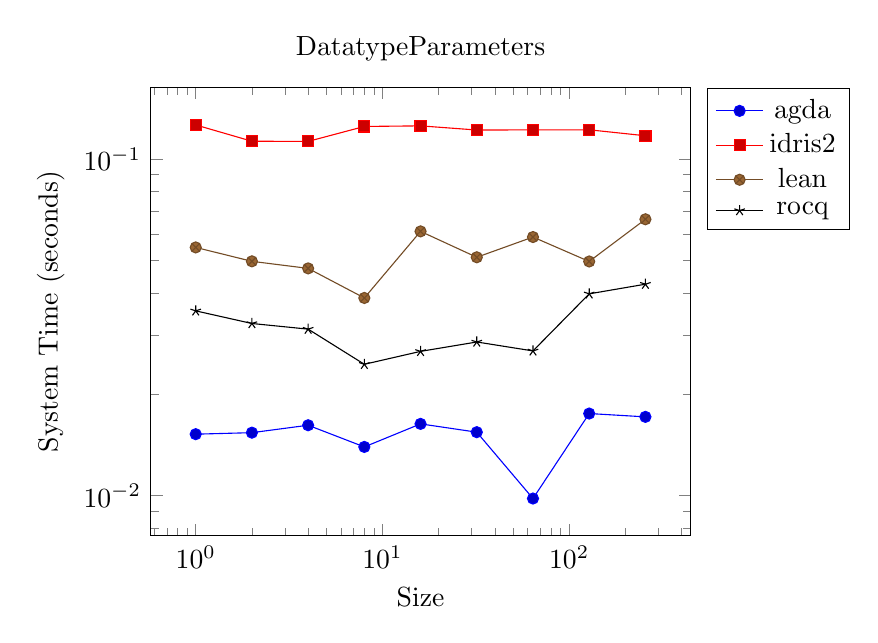
\begin{tikzpicture}
\begin{loglogaxis}
[title=DatatypeParameters,
xlabel={Size},
ylabel={System Time (seconds)},
legend entries={agda,idris2,lean,rocq},
legend pos=outer north east,
]\addplot coordinates {
(256.0,1.7155e-2) [0]
(128.0,1.755e-2) [0]
(64.0,9.813e-3) [0]
(32.0,1.545e-2) [0]
(16.0,1.6352e-2) [0]
(8.0,1.3967e-2) [0]
(4.0,1.62e-2) [0]
(2.0,1.5398e-2) [0]
(1.0,1.524e-2) [0]
};
\addplot coordinates {
(256.0,0.117316) [0]
(128.0,0.122186) [0]
(64.0,0.122117) [0]
(32.0,0.122001) [0]
(16.0,0.125521) [0]
(8.0,0.125017) [0]
(4.0,0.112862) [0]
(2.0,0.112996) [0]
(1.0,0.126323) [0]
};
\addplot coordinates {
(256.0,6.6273e-2) [256]
(128.0,4.9652e-2) [256]
(64.0,5.8684e-2) [0]
(32.0,5.1098e-2) [0]
(16.0,6.1002e-2) [0]
(8.0,3.8694e-2) [0]
(4.0,4.7356e-2) [0]
(2.0,4.9701e-2) [0]
(1.0,5.4661e-2) [0]
};
\addplot coordinates {
(256.0,4.2505e-2) [0]
(128.0,3.9801e-2) [0]
(64.0,2.6931e-2) [0]
(32.0,2.863e-2) [0]
(16.0,2.6848e-2) [0]
(8.0,2.4578e-2) [0]
(4.0,3.1258e-2) [0]
(2.0,3.2489e-2) [0]
(1.0,3.542e-2) [0]
};
\end{loglogaxis}
\end{tikzpicture}

% \\
% 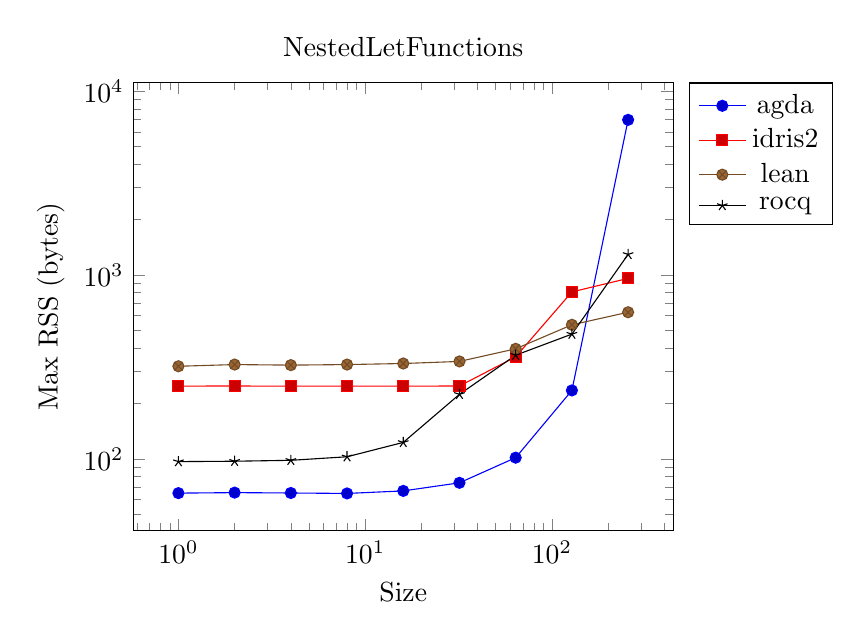
\begin{tikzpicture}
\begin{loglogaxis}
[title=NestedLetFunctions,
xlabel={Size},
ylabel={Max RSS (bytes)},
legend entries={agda,idris2,lean,rocq},
legend pos=outer north east,
]\addplot coordinates {
(256.0,6970.933248) [9]
(128.0,235.630592) [0]
(64.0,101.531648) [0]
(32.0,74.11712) [0]
(16.0,66.9696) [0]
(8.0,64.872448) [0]
(4.0,65.236992) [0]
(2.0,65.548288) [0]
(1.0,65.130496) [0]
};
\addplot coordinates {
(256.0,957.755392) [35072]
(128.0,808.771584) [35072]
(64.0,358.68672) [0]
(32.0,248.905728) [0]
(16.0,248.68864) [0]
(8.0,248.7296) [0]
(4.0,248.684544) [0]
(2.0,248.89344) [0]
(1.0,248.77056) [0]
};
\addplot coordinates {
(256.0,626.950144) [9]
(128.0,535.67488) [9]
(64.0,396.644352) [0]
(32.0,338.702336) [0]
(16.0,329.977856) [0]
(8.0,325.644288) [0]
(4.0,323.387392) [0]
(2.0,325.619712) [0]
(1.0,318.803968) [0]
};
\addplot coordinates {
(256.0,1293.410304) [0]
(128.0,476.749824) [0]
(64.0,366.256128) [0]
(32.0,224.354304) [0]
(16.0,122.884096) [0]
(8.0,102.670336) [0]
(4.0,98.213888) [0]
(2.0,97.087488) [0]
(1.0,96.620544) [0]
};
\end{loglogaxis}
\end{tikzpicture}


% \subsection{LongNameDefinition}
% 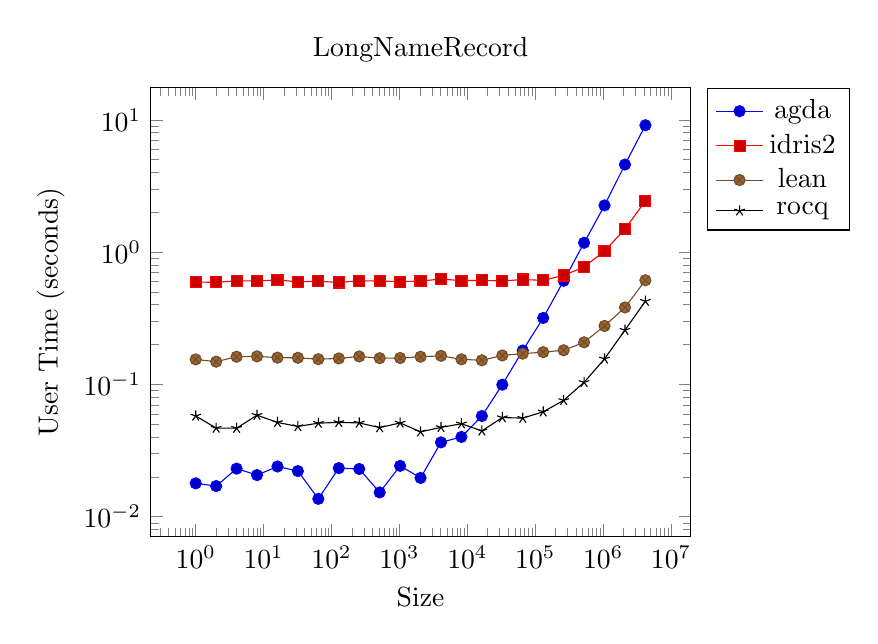
\begin{tikzpicture}
\begin{loglogaxis}
[title=LongNameRecord,
xlabel={Size},
ylabel={User Time (seconds)},
legend entries={agda,idris2,lean,rocq},
legend pos=outer north east,
]\addplot coordinates {
(4194304.0,9.097116) [0]
(2097152.0,4.588252) [0]
(1048576.0,2.253942) [0]
(524288.0,1.175644) [0]
(262144.0,0.606869) [0]
(131072.0,0.318102) [0]
(65536.0,0.180498) [0]
(32768.0,9.9566e-2) [0]
(16384.0,5.7703e-2) [0]
(8192.0,4.0103e-2) [0]
(4096.0,3.6509e-2) [0]
(2048.0,1.9649e-2) [0]
(1024.0,2.4239e-2) [0]
(512.0,1.5274e-2) [0]
(256.0,2.2951e-2) [0]
(128.0,2.3313e-2) [0]
(64.0,1.3655e-2) [0]
(32.0,2.2137e-2) [0]
(16.0,2.3973e-2) [0]
(8.0,2.0647e-2) [0]
(4.0,2.3102e-2) [0]
(2.0,1.7053e-2) [0]
(1.0,1.7885e-2) [0]
};
\addplot coordinates {
(4194304.0,2.435465) [0]
(2097152.0,1.494713) [0]
(1048576.0,1.018833) [0]
(524288.0,0.772144) [0]
(262144.0,0.66665) [0]
(131072.0,0.611889) [0]
(65536.0,0.620374) [0]
(32768.0,0.605496) [0]
(16384.0,0.611539) [0]
(8192.0,0.608788) [0]
(4096.0,0.626241) [0]
(2048.0,0.603874) [0]
(1024.0,0.598415) [0]
(512.0,0.604452) [0]
(256.0,0.60748) [0]
(128.0,0.589608) [0]
(64.0,0.603068) [0]
(32.0,0.596021) [0]
(16.0,0.616476) [0]
(8.0,0.605033) [0]
(4.0,0.606919) [0]
(2.0,0.591078) [0]
(1.0,0.594091) [0]
};
\addplot coordinates {
(4194304.0,0.612912) [0]
(2097152.0,0.381734) [0]
(1048576.0,0.276632) [0]
(524288.0,0.208152) [0]
(262144.0,0.181183) [0]
(131072.0,0.17531) [0]
(65536.0,0.170923) [0]
(32768.0,0.165527) [0]
(16384.0,0.15219) [0]
(8192.0,0.15478) [0]
(4096.0,0.164464) [0]
(2048.0,0.161915) [0]
(1024.0,0.158346) [0]
(512.0,0.157909) [0]
(256.0,0.162727) [0]
(128.0,0.157235) [0]
(64.0,0.155179) [0]
(32.0,0.158943) [0]
(16.0,0.159408) [0]
(8.0,0.162905) [0]
(4.0,0.16191) [0]
(2.0,0.148563) [0]
(1.0,0.15453) [0]
};
\addplot coordinates {
(4194304.0,0.426038) [0]
(2097152.0,0.257224) [0]
(1048576.0,0.156022) [0]
(524288.0,0.103696) [0]
(262144.0,7.5799e-2) [0]
(131072.0,6.2094e-2) [0]
(65536.0,5.5643e-2) [0]
(32768.0,5.6181e-2) [0]
(16384.0,4.4542e-2) [0]
(8192.0,5.0413e-2) [0]
(4096.0,4.7327e-2) [0]
(2048.0,4.3836e-2) [0]
(1024.0,5.1143e-2) [0]
(512.0,4.7186e-2) [0]
(256.0,5.1154e-2) [0]
(128.0,5.1667e-2) [0]
(64.0,5.0968e-2) [0]
(32.0,4.8123e-2) [0]
(16.0,5.1609e-2) [0]
(8.0,5.8562e-2) [0]
(4.0,4.6712e-2) [0]
(2.0,4.6796e-2) [0]
(1.0,5.7777e-2) [0]
};
\end{loglogaxis}
\end{tikzpicture}

% \\
% 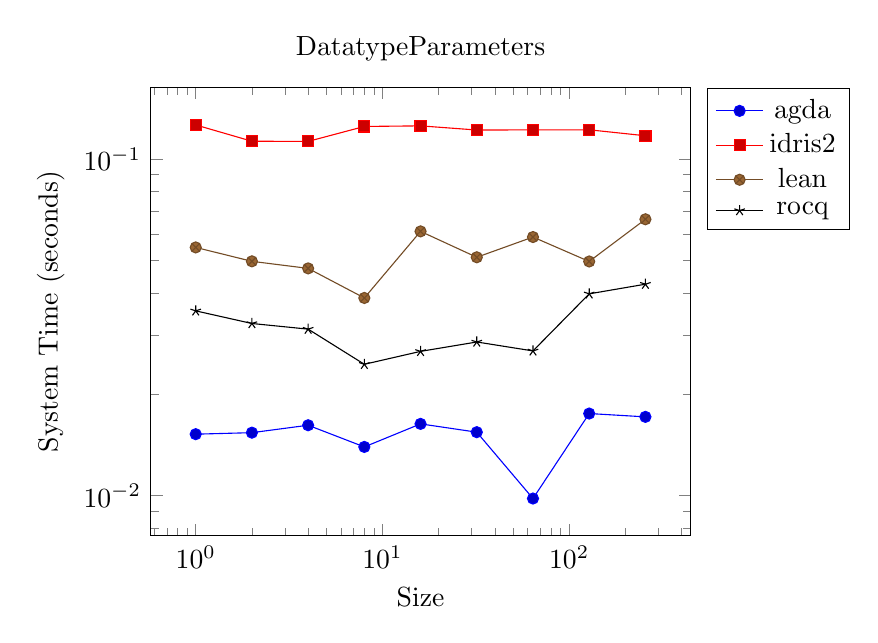
\begin{tikzpicture}
\begin{loglogaxis}
[title=DatatypeParameters,
xlabel={Size},
ylabel={System Time (seconds)},
legend entries={agda,idris2,lean,rocq},
legend pos=outer north east,
]\addplot coordinates {
(256.0,1.7155e-2) [0]
(128.0,1.755e-2) [0]
(64.0,9.813e-3) [0]
(32.0,1.545e-2) [0]
(16.0,1.6352e-2) [0]
(8.0,1.3967e-2) [0]
(4.0,1.62e-2) [0]
(2.0,1.5398e-2) [0]
(1.0,1.524e-2) [0]
};
\addplot coordinates {
(256.0,0.117316) [0]
(128.0,0.122186) [0]
(64.0,0.122117) [0]
(32.0,0.122001) [0]
(16.0,0.125521) [0]
(8.0,0.125017) [0]
(4.0,0.112862) [0]
(2.0,0.112996) [0]
(1.0,0.126323) [0]
};
\addplot coordinates {
(256.0,6.6273e-2) [256]
(128.0,4.9652e-2) [256]
(64.0,5.8684e-2) [0]
(32.0,5.1098e-2) [0]
(16.0,6.1002e-2) [0]
(8.0,3.8694e-2) [0]
(4.0,4.7356e-2) [0]
(2.0,4.9701e-2) [0]
(1.0,5.4661e-2) [0]
};
\addplot coordinates {
(256.0,4.2505e-2) [0]
(128.0,3.9801e-2) [0]
(64.0,2.6931e-2) [0]
(32.0,2.863e-2) [0]
(16.0,2.6848e-2) [0]
(8.0,2.4578e-2) [0]
(4.0,3.1258e-2) [0]
(2.0,3.2489e-2) [0]
(1.0,3.542e-2) [0]
};
\end{loglogaxis}
\end{tikzpicture}

% \\
% 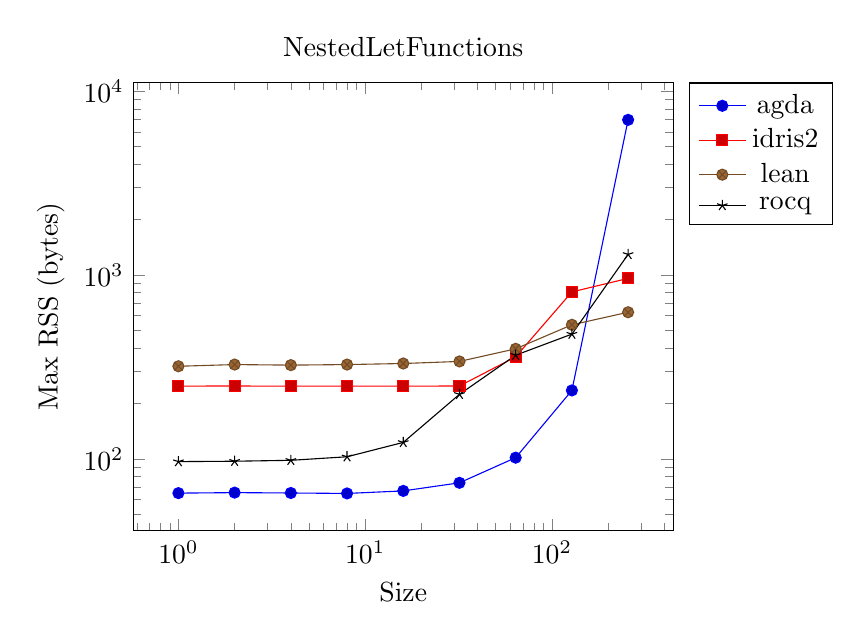
\begin{tikzpicture}
\begin{loglogaxis}
[title=NestedLetFunctions,
xlabel={Size},
ylabel={Max RSS (bytes)},
legend entries={agda,idris2,lean,rocq},
legend pos=outer north east,
]\addplot coordinates {
(256.0,6970.933248) [9]
(128.0,235.630592) [0]
(64.0,101.531648) [0]
(32.0,74.11712) [0]
(16.0,66.9696) [0]
(8.0,64.872448) [0]
(4.0,65.236992) [0]
(2.0,65.548288) [0]
(1.0,65.130496) [0]
};
\addplot coordinates {
(256.0,957.755392) [35072]
(128.0,808.771584) [35072]
(64.0,358.68672) [0]
(32.0,248.905728) [0]
(16.0,248.68864) [0]
(8.0,248.7296) [0]
(4.0,248.684544) [0]
(2.0,248.89344) [0]
(1.0,248.77056) [0]
};
\addplot coordinates {
(256.0,626.950144) [9]
(128.0,535.67488) [9]
(64.0,396.644352) [0]
(32.0,338.702336) [0]
(16.0,329.977856) [0]
(8.0,325.644288) [0]
(4.0,323.387392) [0]
(2.0,325.619712) [0]
(1.0,318.803968) [0]
};
\addplot coordinates {
(256.0,1293.410304) [0]
(128.0,476.749824) [0]
(64.0,366.256128) [0]
(32.0,224.354304) [0]
(16.0,122.884096) [0]
(8.0,102.670336) [0]
(4.0,98.213888) [0]
(2.0,97.087488) [0]
(1.0,96.620544) [0]
};
\end{loglogaxis}
\end{tikzpicture}


% \subsection{LongNameDefinitionLhs}
% 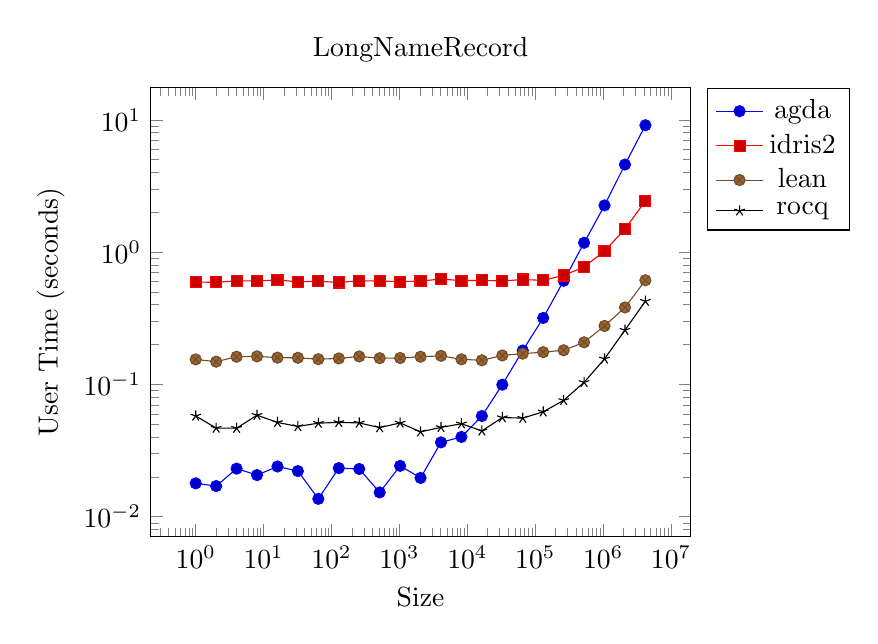
\begin{tikzpicture}
\begin{loglogaxis}
[title=LongNameRecord,
xlabel={Size},
ylabel={User Time (seconds)},
legend entries={agda,idris2,lean,rocq},
legend pos=outer north east,
]\addplot coordinates {
(4194304.0,9.097116) [0]
(2097152.0,4.588252) [0]
(1048576.0,2.253942) [0]
(524288.0,1.175644) [0]
(262144.0,0.606869) [0]
(131072.0,0.318102) [0]
(65536.0,0.180498) [0]
(32768.0,9.9566e-2) [0]
(16384.0,5.7703e-2) [0]
(8192.0,4.0103e-2) [0]
(4096.0,3.6509e-2) [0]
(2048.0,1.9649e-2) [0]
(1024.0,2.4239e-2) [0]
(512.0,1.5274e-2) [0]
(256.0,2.2951e-2) [0]
(128.0,2.3313e-2) [0]
(64.0,1.3655e-2) [0]
(32.0,2.2137e-2) [0]
(16.0,2.3973e-2) [0]
(8.0,2.0647e-2) [0]
(4.0,2.3102e-2) [0]
(2.0,1.7053e-2) [0]
(1.0,1.7885e-2) [0]
};
\addplot coordinates {
(4194304.0,2.435465) [0]
(2097152.0,1.494713) [0]
(1048576.0,1.018833) [0]
(524288.0,0.772144) [0]
(262144.0,0.66665) [0]
(131072.0,0.611889) [0]
(65536.0,0.620374) [0]
(32768.0,0.605496) [0]
(16384.0,0.611539) [0]
(8192.0,0.608788) [0]
(4096.0,0.626241) [0]
(2048.0,0.603874) [0]
(1024.0,0.598415) [0]
(512.0,0.604452) [0]
(256.0,0.60748) [0]
(128.0,0.589608) [0]
(64.0,0.603068) [0]
(32.0,0.596021) [0]
(16.0,0.616476) [0]
(8.0,0.605033) [0]
(4.0,0.606919) [0]
(2.0,0.591078) [0]
(1.0,0.594091) [0]
};
\addplot coordinates {
(4194304.0,0.612912) [0]
(2097152.0,0.381734) [0]
(1048576.0,0.276632) [0]
(524288.0,0.208152) [0]
(262144.0,0.181183) [0]
(131072.0,0.17531) [0]
(65536.0,0.170923) [0]
(32768.0,0.165527) [0]
(16384.0,0.15219) [0]
(8192.0,0.15478) [0]
(4096.0,0.164464) [0]
(2048.0,0.161915) [0]
(1024.0,0.158346) [0]
(512.0,0.157909) [0]
(256.0,0.162727) [0]
(128.0,0.157235) [0]
(64.0,0.155179) [0]
(32.0,0.158943) [0]
(16.0,0.159408) [0]
(8.0,0.162905) [0]
(4.0,0.16191) [0]
(2.0,0.148563) [0]
(1.0,0.15453) [0]
};
\addplot coordinates {
(4194304.0,0.426038) [0]
(2097152.0,0.257224) [0]
(1048576.0,0.156022) [0]
(524288.0,0.103696) [0]
(262144.0,7.5799e-2) [0]
(131072.0,6.2094e-2) [0]
(65536.0,5.5643e-2) [0]
(32768.0,5.6181e-2) [0]
(16384.0,4.4542e-2) [0]
(8192.0,5.0413e-2) [0]
(4096.0,4.7327e-2) [0]
(2048.0,4.3836e-2) [0]
(1024.0,5.1143e-2) [0]
(512.0,4.7186e-2) [0]
(256.0,5.1154e-2) [0]
(128.0,5.1667e-2) [0]
(64.0,5.0968e-2) [0]
(32.0,4.8123e-2) [0]
(16.0,5.1609e-2) [0]
(8.0,5.8562e-2) [0]
(4.0,4.6712e-2) [0]
(2.0,4.6796e-2) [0]
(1.0,5.7777e-2) [0]
};
\end{loglogaxis}
\end{tikzpicture}

% \\
% 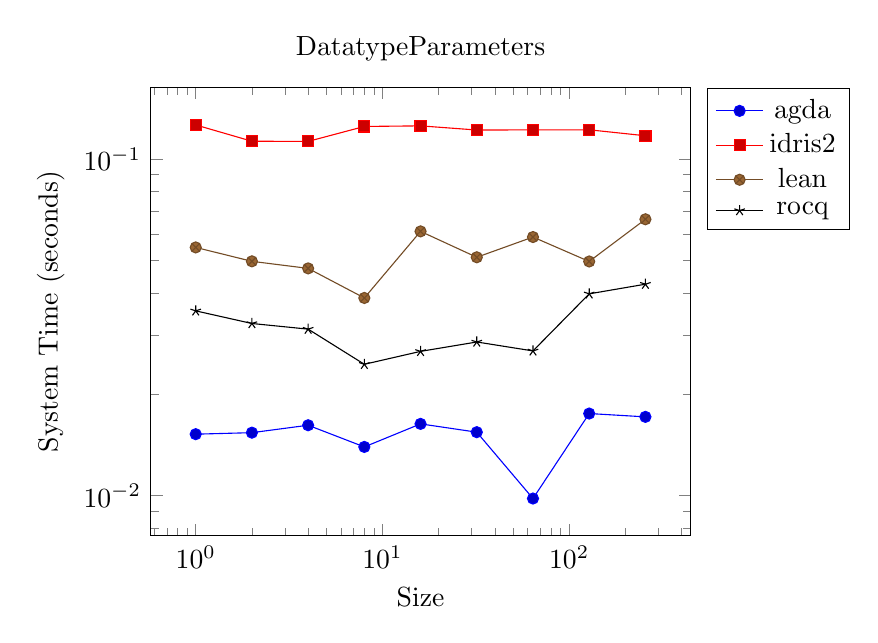
\begin{tikzpicture}
\begin{loglogaxis}
[title=DatatypeParameters,
xlabel={Size},
ylabel={System Time (seconds)},
legend entries={agda,idris2,lean,rocq},
legend pos=outer north east,
]\addplot coordinates {
(256.0,1.7155e-2) [0]
(128.0,1.755e-2) [0]
(64.0,9.813e-3) [0]
(32.0,1.545e-2) [0]
(16.0,1.6352e-2) [0]
(8.0,1.3967e-2) [0]
(4.0,1.62e-2) [0]
(2.0,1.5398e-2) [0]
(1.0,1.524e-2) [0]
};
\addplot coordinates {
(256.0,0.117316) [0]
(128.0,0.122186) [0]
(64.0,0.122117) [0]
(32.0,0.122001) [0]
(16.0,0.125521) [0]
(8.0,0.125017) [0]
(4.0,0.112862) [0]
(2.0,0.112996) [0]
(1.0,0.126323) [0]
};
\addplot coordinates {
(256.0,6.6273e-2) [256]
(128.0,4.9652e-2) [256]
(64.0,5.8684e-2) [0]
(32.0,5.1098e-2) [0]
(16.0,6.1002e-2) [0]
(8.0,3.8694e-2) [0]
(4.0,4.7356e-2) [0]
(2.0,4.9701e-2) [0]
(1.0,5.4661e-2) [0]
};
\addplot coordinates {
(256.0,4.2505e-2) [0]
(128.0,3.9801e-2) [0]
(64.0,2.6931e-2) [0]
(32.0,2.863e-2) [0]
(16.0,2.6848e-2) [0]
(8.0,2.4578e-2) [0]
(4.0,3.1258e-2) [0]
(2.0,3.2489e-2) [0]
(1.0,3.542e-2) [0]
};
\end{loglogaxis}
\end{tikzpicture}

% \\
% 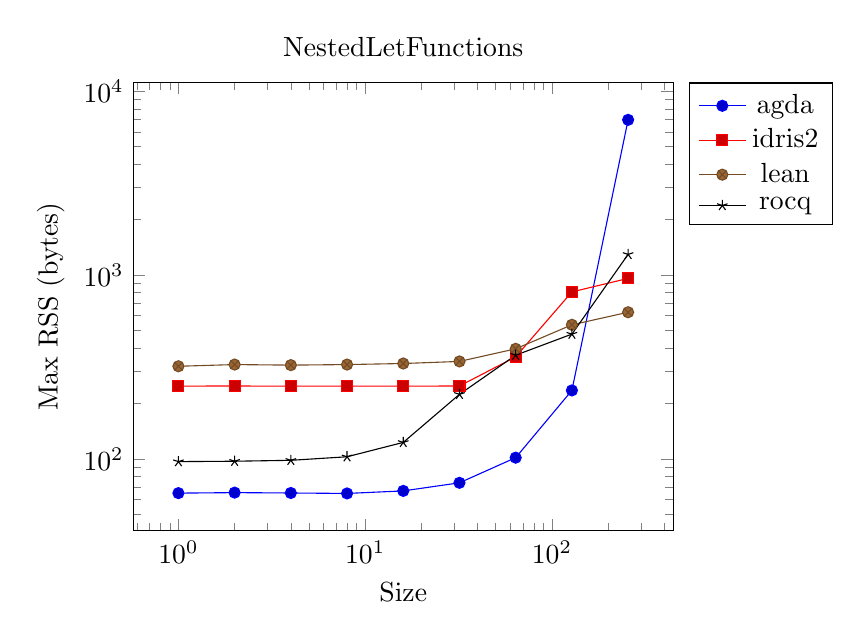
\begin{tikzpicture}
\begin{loglogaxis}
[title=NestedLetFunctions,
xlabel={Size},
ylabel={Max RSS (bytes)},
legend entries={agda,idris2,lean,rocq},
legend pos=outer north east,
]\addplot coordinates {
(256.0,6970.933248) [9]
(128.0,235.630592) [0]
(64.0,101.531648) [0]
(32.0,74.11712) [0]
(16.0,66.9696) [0]
(8.0,64.872448) [0]
(4.0,65.236992) [0]
(2.0,65.548288) [0]
(1.0,65.130496) [0]
};
\addplot coordinates {
(256.0,957.755392) [35072]
(128.0,808.771584) [35072]
(64.0,358.68672) [0]
(32.0,248.905728) [0]
(16.0,248.68864) [0]
(8.0,248.7296) [0]
(4.0,248.684544) [0]
(2.0,248.89344) [0]
(1.0,248.77056) [0]
};
\addplot coordinates {
(256.0,626.950144) [9]
(128.0,535.67488) [9]
(64.0,396.644352) [0]
(32.0,338.702336) [0]
(16.0,329.977856) [0]
(8.0,325.644288) [0]
(4.0,323.387392) [0]
(2.0,325.619712) [0]
(1.0,318.803968) [0]
};
\addplot coordinates {
(256.0,1293.410304) [0]
(128.0,476.749824) [0]
(64.0,366.256128) [0]
(32.0,224.354304) [0]
(16.0,122.884096) [0]
(8.0,102.670336) [0]
(4.0,98.213888) [0]
(2.0,97.087488) [0]
(1.0,96.620544) [0]
};
\end{loglogaxis}
\end{tikzpicture}


% \subsection{LongNameDefinitionRhs}
% 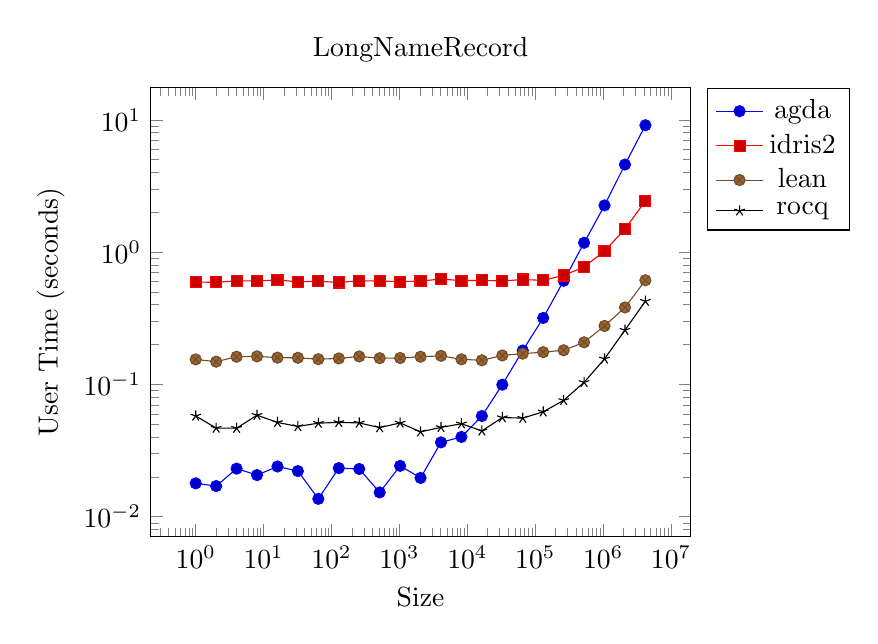
\begin{tikzpicture}
\begin{loglogaxis}
[title=LongNameRecord,
xlabel={Size},
ylabel={User Time (seconds)},
legend entries={agda,idris2,lean,rocq},
legend pos=outer north east,
]\addplot coordinates {
(4194304.0,9.097116) [0]
(2097152.0,4.588252) [0]
(1048576.0,2.253942) [0]
(524288.0,1.175644) [0]
(262144.0,0.606869) [0]
(131072.0,0.318102) [0]
(65536.0,0.180498) [0]
(32768.0,9.9566e-2) [0]
(16384.0,5.7703e-2) [0]
(8192.0,4.0103e-2) [0]
(4096.0,3.6509e-2) [0]
(2048.0,1.9649e-2) [0]
(1024.0,2.4239e-2) [0]
(512.0,1.5274e-2) [0]
(256.0,2.2951e-2) [0]
(128.0,2.3313e-2) [0]
(64.0,1.3655e-2) [0]
(32.0,2.2137e-2) [0]
(16.0,2.3973e-2) [0]
(8.0,2.0647e-2) [0]
(4.0,2.3102e-2) [0]
(2.0,1.7053e-2) [0]
(1.0,1.7885e-2) [0]
};
\addplot coordinates {
(4194304.0,2.435465) [0]
(2097152.0,1.494713) [0]
(1048576.0,1.018833) [0]
(524288.0,0.772144) [0]
(262144.0,0.66665) [0]
(131072.0,0.611889) [0]
(65536.0,0.620374) [0]
(32768.0,0.605496) [0]
(16384.0,0.611539) [0]
(8192.0,0.608788) [0]
(4096.0,0.626241) [0]
(2048.0,0.603874) [0]
(1024.0,0.598415) [0]
(512.0,0.604452) [0]
(256.0,0.60748) [0]
(128.0,0.589608) [0]
(64.0,0.603068) [0]
(32.0,0.596021) [0]
(16.0,0.616476) [0]
(8.0,0.605033) [0]
(4.0,0.606919) [0]
(2.0,0.591078) [0]
(1.0,0.594091) [0]
};
\addplot coordinates {
(4194304.0,0.612912) [0]
(2097152.0,0.381734) [0]
(1048576.0,0.276632) [0]
(524288.0,0.208152) [0]
(262144.0,0.181183) [0]
(131072.0,0.17531) [0]
(65536.0,0.170923) [0]
(32768.0,0.165527) [0]
(16384.0,0.15219) [0]
(8192.0,0.15478) [0]
(4096.0,0.164464) [0]
(2048.0,0.161915) [0]
(1024.0,0.158346) [0]
(512.0,0.157909) [0]
(256.0,0.162727) [0]
(128.0,0.157235) [0]
(64.0,0.155179) [0]
(32.0,0.158943) [0]
(16.0,0.159408) [0]
(8.0,0.162905) [0]
(4.0,0.16191) [0]
(2.0,0.148563) [0]
(1.0,0.15453) [0]
};
\addplot coordinates {
(4194304.0,0.426038) [0]
(2097152.0,0.257224) [0]
(1048576.0,0.156022) [0]
(524288.0,0.103696) [0]
(262144.0,7.5799e-2) [0]
(131072.0,6.2094e-2) [0]
(65536.0,5.5643e-2) [0]
(32768.0,5.6181e-2) [0]
(16384.0,4.4542e-2) [0]
(8192.0,5.0413e-2) [0]
(4096.0,4.7327e-2) [0]
(2048.0,4.3836e-2) [0]
(1024.0,5.1143e-2) [0]
(512.0,4.7186e-2) [0]
(256.0,5.1154e-2) [0]
(128.0,5.1667e-2) [0]
(64.0,5.0968e-2) [0]
(32.0,4.8123e-2) [0]
(16.0,5.1609e-2) [0]
(8.0,5.8562e-2) [0]
(4.0,4.6712e-2) [0]
(2.0,4.6796e-2) [0]
(1.0,5.7777e-2) [0]
};
\end{loglogaxis}
\end{tikzpicture}

% \\
% 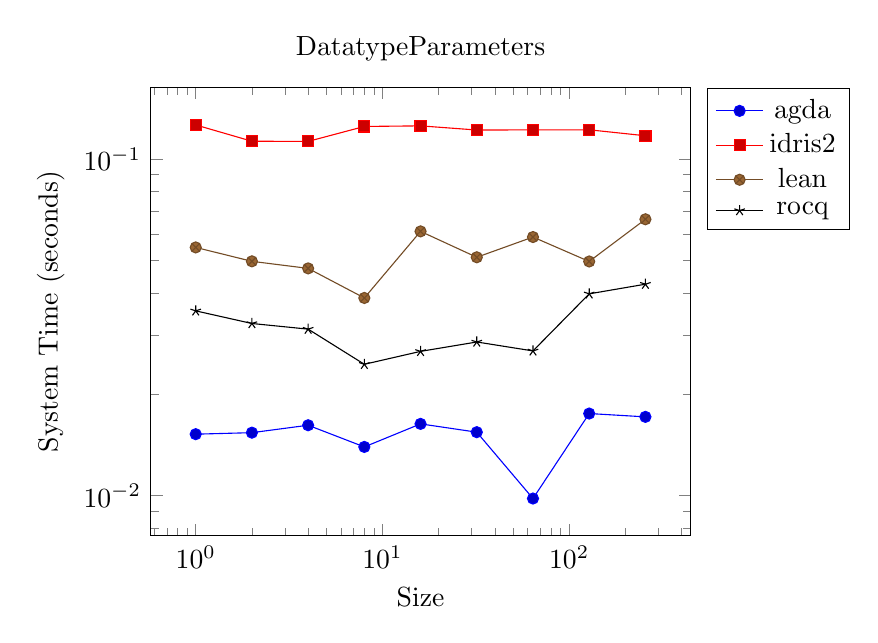
\begin{tikzpicture}
\begin{loglogaxis}
[title=DatatypeParameters,
xlabel={Size},
ylabel={System Time (seconds)},
legend entries={agda,idris2,lean,rocq},
legend pos=outer north east,
]\addplot coordinates {
(256.0,1.7155e-2) [0]
(128.0,1.755e-2) [0]
(64.0,9.813e-3) [0]
(32.0,1.545e-2) [0]
(16.0,1.6352e-2) [0]
(8.0,1.3967e-2) [0]
(4.0,1.62e-2) [0]
(2.0,1.5398e-2) [0]
(1.0,1.524e-2) [0]
};
\addplot coordinates {
(256.0,0.117316) [0]
(128.0,0.122186) [0]
(64.0,0.122117) [0]
(32.0,0.122001) [0]
(16.0,0.125521) [0]
(8.0,0.125017) [0]
(4.0,0.112862) [0]
(2.0,0.112996) [0]
(1.0,0.126323) [0]
};
\addplot coordinates {
(256.0,6.6273e-2) [256]
(128.0,4.9652e-2) [256]
(64.0,5.8684e-2) [0]
(32.0,5.1098e-2) [0]
(16.0,6.1002e-2) [0]
(8.0,3.8694e-2) [0]
(4.0,4.7356e-2) [0]
(2.0,4.9701e-2) [0]
(1.0,5.4661e-2) [0]
};
\addplot coordinates {
(256.0,4.2505e-2) [0]
(128.0,3.9801e-2) [0]
(64.0,2.6931e-2) [0]
(32.0,2.863e-2) [0]
(16.0,2.6848e-2) [0]
(8.0,2.4578e-2) [0]
(4.0,3.1258e-2) [0]
(2.0,3.2489e-2) [0]
(1.0,3.542e-2) [0]
};
\end{loglogaxis}
\end{tikzpicture}

% \\
% 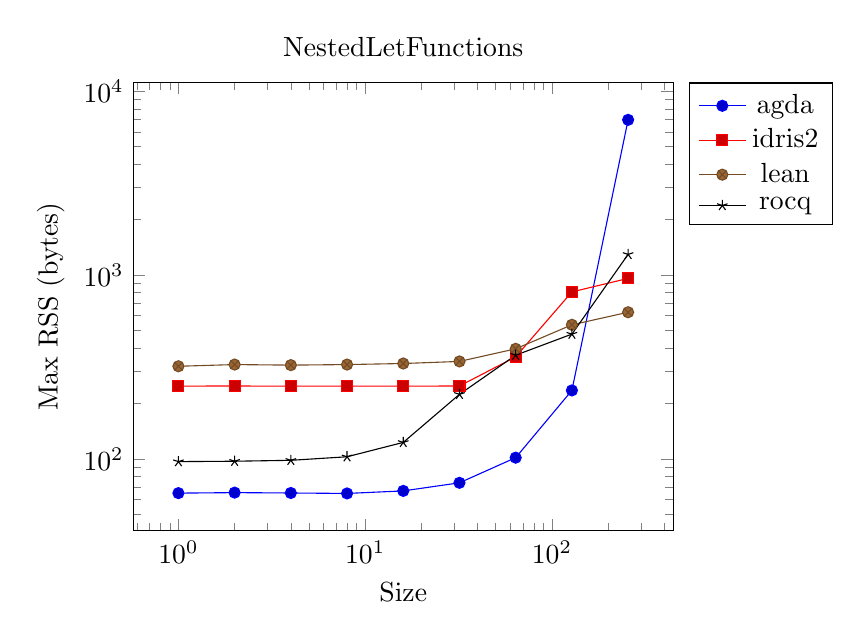
\begin{tikzpicture}
\begin{loglogaxis}
[title=NestedLetFunctions,
xlabel={Size},
ylabel={Max RSS (bytes)},
legend entries={agda,idris2,lean,rocq},
legend pos=outer north east,
]\addplot coordinates {
(256.0,6970.933248) [9]
(128.0,235.630592) [0]
(64.0,101.531648) [0]
(32.0,74.11712) [0]
(16.0,66.9696) [0]
(8.0,64.872448) [0]
(4.0,65.236992) [0]
(2.0,65.548288) [0]
(1.0,65.130496) [0]
};
\addplot coordinates {
(256.0,957.755392) [35072]
(128.0,808.771584) [35072]
(64.0,358.68672) [0]
(32.0,248.905728) [0]
(16.0,248.68864) [0]
(8.0,248.7296) [0]
(4.0,248.684544) [0]
(2.0,248.89344) [0]
(1.0,248.77056) [0]
};
\addplot coordinates {
(256.0,626.950144) [9]
(128.0,535.67488) [9]
(64.0,396.644352) [0]
(32.0,338.702336) [0]
(16.0,329.977856) [0]
(8.0,325.644288) [0]
(4.0,323.387392) [0]
(2.0,325.619712) [0]
(1.0,318.803968) [0]
};
\addplot coordinates {
(256.0,1293.410304) [0]
(128.0,476.749824) [0]
(64.0,366.256128) [0]
(32.0,224.354304) [0]
(16.0,122.884096) [0]
(8.0,102.670336) [0]
(4.0,98.213888) [0]
(2.0,97.087488) [0]
(1.0,96.620544) [0]
};
\end{loglogaxis}
\end{tikzpicture}


% \subsection{LongNameLambda}
% 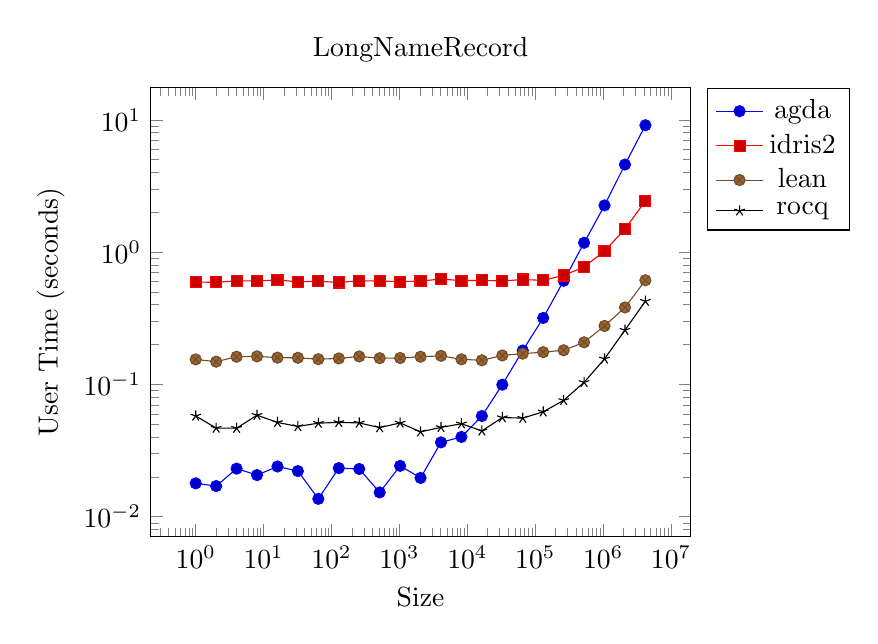
\begin{tikzpicture}
\begin{loglogaxis}
[title=LongNameRecord,
xlabel={Size},
ylabel={User Time (seconds)},
legend entries={agda,idris2,lean,rocq},
legend pos=outer north east,
]\addplot coordinates {
(4194304.0,9.097116) [0]
(2097152.0,4.588252) [0]
(1048576.0,2.253942) [0]
(524288.0,1.175644) [0]
(262144.0,0.606869) [0]
(131072.0,0.318102) [0]
(65536.0,0.180498) [0]
(32768.0,9.9566e-2) [0]
(16384.0,5.7703e-2) [0]
(8192.0,4.0103e-2) [0]
(4096.0,3.6509e-2) [0]
(2048.0,1.9649e-2) [0]
(1024.0,2.4239e-2) [0]
(512.0,1.5274e-2) [0]
(256.0,2.2951e-2) [0]
(128.0,2.3313e-2) [0]
(64.0,1.3655e-2) [0]
(32.0,2.2137e-2) [0]
(16.0,2.3973e-2) [0]
(8.0,2.0647e-2) [0]
(4.0,2.3102e-2) [0]
(2.0,1.7053e-2) [0]
(1.0,1.7885e-2) [0]
};
\addplot coordinates {
(4194304.0,2.435465) [0]
(2097152.0,1.494713) [0]
(1048576.0,1.018833) [0]
(524288.0,0.772144) [0]
(262144.0,0.66665) [0]
(131072.0,0.611889) [0]
(65536.0,0.620374) [0]
(32768.0,0.605496) [0]
(16384.0,0.611539) [0]
(8192.0,0.608788) [0]
(4096.0,0.626241) [0]
(2048.0,0.603874) [0]
(1024.0,0.598415) [0]
(512.0,0.604452) [0]
(256.0,0.60748) [0]
(128.0,0.589608) [0]
(64.0,0.603068) [0]
(32.0,0.596021) [0]
(16.0,0.616476) [0]
(8.0,0.605033) [0]
(4.0,0.606919) [0]
(2.0,0.591078) [0]
(1.0,0.594091) [0]
};
\addplot coordinates {
(4194304.0,0.612912) [0]
(2097152.0,0.381734) [0]
(1048576.0,0.276632) [0]
(524288.0,0.208152) [0]
(262144.0,0.181183) [0]
(131072.0,0.17531) [0]
(65536.0,0.170923) [0]
(32768.0,0.165527) [0]
(16384.0,0.15219) [0]
(8192.0,0.15478) [0]
(4096.0,0.164464) [0]
(2048.0,0.161915) [0]
(1024.0,0.158346) [0]
(512.0,0.157909) [0]
(256.0,0.162727) [0]
(128.0,0.157235) [0]
(64.0,0.155179) [0]
(32.0,0.158943) [0]
(16.0,0.159408) [0]
(8.0,0.162905) [0]
(4.0,0.16191) [0]
(2.0,0.148563) [0]
(1.0,0.15453) [0]
};
\addplot coordinates {
(4194304.0,0.426038) [0]
(2097152.0,0.257224) [0]
(1048576.0,0.156022) [0]
(524288.0,0.103696) [0]
(262144.0,7.5799e-2) [0]
(131072.0,6.2094e-2) [0]
(65536.0,5.5643e-2) [0]
(32768.0,5.6181e-2) [0]
(16384.0,4.4542e-2) [0]
(8192.0,5.0413e-2) [0]
(4096.0,4.7327e-2) [0]
(2048.0,4.3836e-2) [0]
(1024.0,5.1143e-2) [0]
(512.0,4.7186e-2) [0]
(256.0,5.1154e-2) [0]
(128.0,5.1667e-2) [0]
(64.0,5.0968e-2) [0]
(32.0,4.8123e-2) [0]
(16.0,5.1609e-2) [0]
(8.0,5.8562e-2) [0]
(4.0,4.6712e-2) [0]
(2.0,4.6796e-2) [0]
(1.0,5.7777e-2) [0]
};
\end{loglogaxis}
\end{tikzpicture}

% \\
% 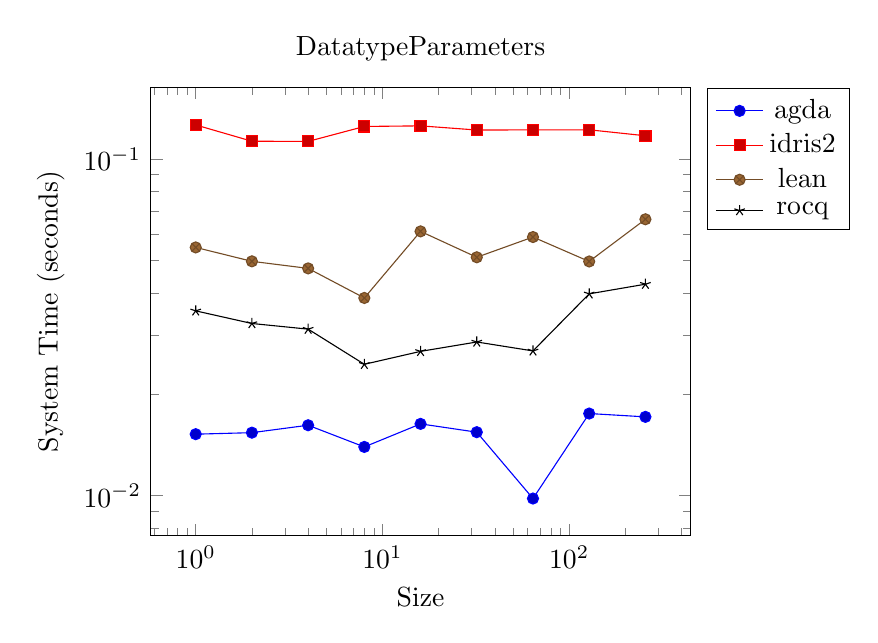
\begin{tikzpicture}
\begin{loglogaxis}
[title=DatatypeParameters,
xlabel={Size},
ylabel={System Time (seconds)},
legend entries={agda,idris2,lean,rocq},
legend pos=outer north east,
]\addplot coordinates {
(256.0,1.7155e-2) [0]
(128.0,1.755e-2) [0]
(64.0,9.813e-3) [0]
(32.0,1.545e-2) [0]
(16.0,1.6352e-2) [0]
(8.0,1.3967e-2) [0]
(4.0,1.62e-2) [0]
(2.0,1.5398e-2) [0]
(1.0,1.524e-2) [0]
};
\addplot coordinates {
(256.0,0.117316) [0]
(128.0,0.122186) [0]
(64.0,0.122117) [0]
(32.0,0.122001) [0]
(16.0,0.125521) [0]
(8.0,0.125017) [0]
(4.0,0.112862) [0]
(2.0,0.112996) [0]
(1.0,0.126323) [0]
};
\addplot coordinates {
(256.0,6.6273e-2) [256]
(128.0,4.9652e-2) [256]
(64.0,5.8684e-2) [0]
(32.0,5.1098e-2) [0]
(16.0,6.1002e-2) [0]
(8.0,3.8694e-2) [0]
(4.0,4.7356e-2) [0]
(2.0,4.9701e-2) [0]
(1.0,5.4661e-2) [0]
};
\addplot coordinates {
(256.0,4.2505e-2) [0]
(128.0,3.9801e-2) [0]
(64.0,2.6931e-2) [0]
(32.0,2.863e-2) [0]
(16.0,2.6848e-2) [0]
(8.0,2.4578e-2) [0]
(4.0,3.1258e-2) [0]
(2.0,3.2489e-2) [0]
(1.0,3.542e-2) [0]
};
\end{loglogaxis}
\end{tikzpicture}

% \\
% 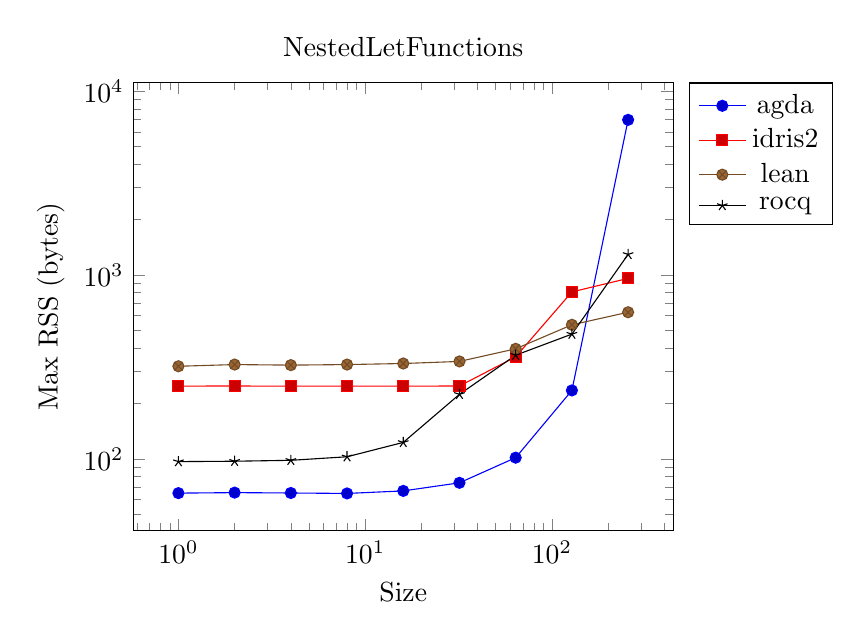
\begin{tikzpicture}
\begin{loglogaxis}
[title=NestedLetFunctions,
xlabel={Size},
ylabel={Max RSS (bytes)},
legend entries={agda,idris2,lean,rocq},
legend pos=outer north east,
]\addplot coordinates {
(256.0,6970.933248) [9]
(128.0,235.630592) [0]
(64.0,101.531648) [0]
(32.0,74.11712) [0]
(16.0,66.9696) [0]
(8.0,64.872448) [0]
(4.0,65.236992) [0]
(2.0,65.548288) [0]
(1.0,65.130496) [0]
};
\addplot coordinates {
(256.0,957.755392) [35072]
(128.0,808.771584) [35072]
(64.0,358.68672) [0]
(32.0,248.905728) [0]
(16.0,248.68864) [0]
(8.0,248.7296) [0]
(4.0,248.684544) [0]
(2.0,248.89344) [0]
(1.0,248.77056) [0]
};
\addplot coordinates {
(256.0,626.950144) [9]
(128.0,535.67488) [9]
(64.0,396.644352) [0]
(32.0,338.702336) [0]
(16.0,329.977856) [0]
(8.0,325.644288) [0]
(4.0,323.387392) [0]
(2.0,325.619712) [0]
(1.0,318.803968) [0]
};
\addplot coordinates {
(256.0,1293.410304) [0]
(128.0,476.749824) [0]
(64.0,366.256128) [0]
(32.0,224.354304) [0]
(16.0,122.884096) [0]
(8.0,102.670336) [0]
(4.0,98.213888) [0]
(2.0,97.087488) [0]
(1.0,96.620544) [0]
};
\end{loglogaxis}
\end{tikzpicture}


% \subsection{LongNamePi}
% 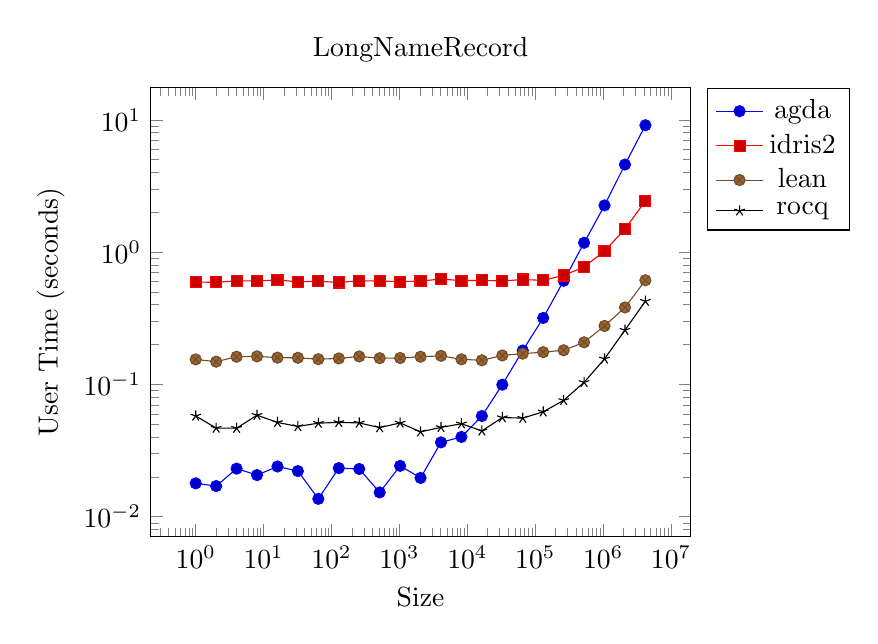
\begin{tikzpicture}
\begin{loglogaxis}
[title=LongNameRecord,
xlabel={Size},
ylabel={User Time (seconds)},
legend entries={agda,idris2,lean,rocq},
legend pos=outer north east,
]\addplot coordinates {
(4194304.0,9.097116) [0]
(2097152.0,4.588252) [0]
(1048576.0,2.253942) [0]
(524288.0,1.175644) [0]
(262144.0,0.606869) [0]
(131072.0,0.318102) [0]
(65536.0,0.180498) [0]
(32768.0,9.9566e-2) [0]
(16384.0,5.7703e-2) [0]
(8192.0,4.0103e-2) [0]
(4096.0,3.6509e-2) [0]
(2048.0,1.9649e-2) [0]
(1024.0,2.4239e-2) [0]
(512.0,1.5274e-2) [0]
(256.0,2.2951e-2) [0]
(128.0,2.3313e-2) [0]
(64.0,1.3655e-2) [0]
(32.0,2.2137e-2) [0]
(16.0,2.3973e-2) [0]
(8.0,2.0647e-2) [0]
(4.0,2.3102e-2) [0]
(2.0,1.7053e-2) [0]
(1.0,1.7885e-2) [0]
};
\addplot coordinates {
(4194304.0,2.435465) [0]
(2097152.0,1.494713) [0]
(1048576.0,1.018833) [0]
(524288.0,0.772144) [0]
(262144.0,0.66665) [0]
(131072.0,0.611889) [0]
(65536.0,0.620374) [0]
(32768.0,0.605496) [0]
(16384.0,0.611539) [0]
(8192.0,0.608788) [0]
(4096.0,0.626241) [0]
(2048.0,0.603874) [0]
(1024.0,0.598415) [0]
(512.0,0.604452) [0]
(256.0,0.60748) [0]
(128.0,0.589608) [0]
(64.0,0.603068) [0]
(32.0,0.596021) [0]
(16.0,0.616476) [0]
(8.0,0.605033) [0]
(4.0,0.606919) [0]
(2.0,0.591078) [0]
(1.0,0.594091) [0]
};
\addplot coordinates {
(4194304.0,0.612912) [0]
(2097152.0,0.381734) [0]
(1048576.0,0.276632) [0]
(524288.0,0.208152) [0]
(262144.0,0.181183) [0]
(131072.0,0.17531) [0]
(65536.0,0.170923) [0]
(32768.0,0.165527) [0]
(16384.0,0.15219) [0]
(8192.0,0.15478) [0]
(4096.0,0.164464) [0]
(2048.0,0.161915) [0]
(1024.0,0.158346) [0]
(512.0,0.157909) [0]
(256.0,0.162727) [0]
(128.0,0.157235) [0]
(64.0,0.155179) [0]
(32.0,0.158943) [0]
(16.0,0.159408) [0]
(8.0,0.162905) [0]
(4.0,0.16191) [0]
(2.0,0.148563) [0]
(1.0,0.15453) [0]
};
\addplot coordinates {
(4194304.0,0.426038) [0]
(2097152.0,0.257224) [0]
(1048576.0,0.156022) [0]
(524288.0,0.103696) [0]
(262144.0,7.5799e-2) [0]
(131072.0,6.2094e-2) [0]
(65536.0,5.5643e-2) [0]
(32768.0,5.6181e-2) [0]
(16384.0,4.4542e-2) [0]
(8192.0,5.0413e-2) [0]
(4096.0,4.7327e-2) [0]
(2048.0,4.3836e-2) [0]
(1024.0,5.1143e-2) [0]
(512.0,4.7186e-2) [0]
(256.0,5.1154e-2) [0]
(128.0,5.1667e-2) [0]
(64.0,5.0968e-2) [0]
(32.0,4.8123e-2) [0]
(16.0,5.1609e-2) [0]
(8.0,5.8562e-2) [0]
(4.0,4.6712e-2) [0]
(2.0,4.6796e-2) [0]
(1.0,5.7777e-2) [0]
};
\end{loglogaxis}
\end{tikzpicture}

% \\
% 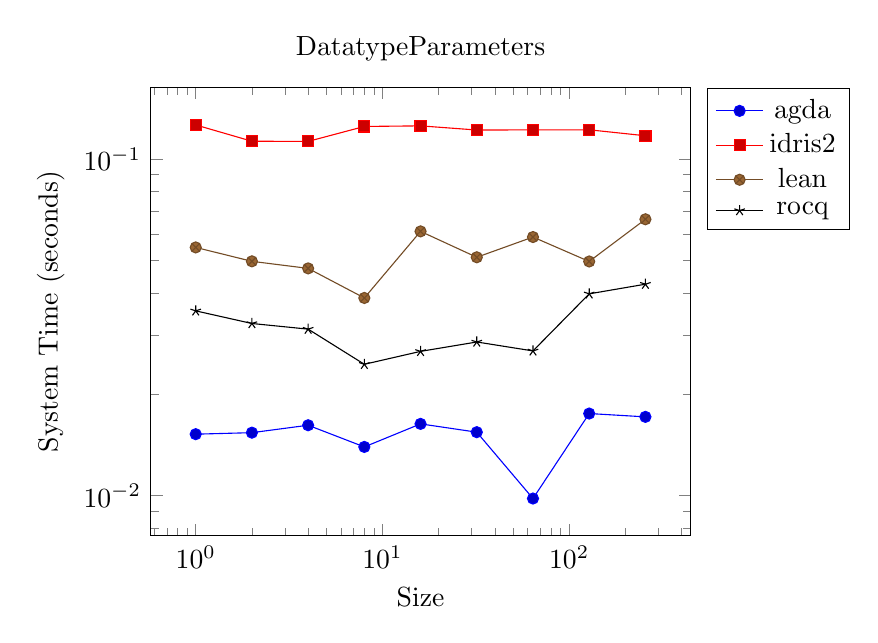
\begin{tikzpicture}
\begin{loglogaxis}
[title=DatatypeParameters,
xlabel={Size},
ylabel={System Time (seconds)},
legend entries={agda,idris2,lean,rocq},
legend pos=outer north east,
]\addplot coordinates {
(256.0,1.7155e-2) [0]
(128.0,1.755e-2) [0]
(64.0,9.813e-3) [0]
(32.0,1.545e-2) [0]
(16.0,1.6352e-2) [0]
(8.0,1.3967e-2) [0]
(4.0,1.62e-2) [0]
(2.0,1.5398e-2) [0]
(1.0,1.524e-2) [0]
};
\addplot coordinates {
(256.0,0.117316) [0]
(128.0,0.122186) [0]
(64.0,0.122117) [0]
(32.0,0.122001) [0]
(16.0,0.125521) [0]
(8.0,0.125017) [0]
(4.0,0.112862) [0]
(2.0,0.112996) [0]
(1.0,0.126323) [0]
};
\addplot coordinates {
(256.0,6.6273e-2) [256]
(128.0,4.9652e-2) [256]
(64.0,5.8684e-2) [0]
(32.0,5.1098e-2) [0]
(16.0,6.1002e-2) [0]
(8.0,3.8694e-2) [0]
(4.0,4.7356e-2) [0]
(2.0,4.9701e-2) [0]
(1.0,5.4661e-2) [0]
};
\addplot coordinates {
(256.0,4.2505e-2) [0]
(128.0,3.9801e-2) [0]
(64.0,2.6931e-2) [0]
(32.0,2.863e-2) [0]
(16.0,2.6848e-2) [0]
(8.0,2.4578e-2) [0]
(4.0,3.1258e-2) [0]
(2.0,3.2489e-2) [0]
(1.0,3.542e-2) [0]
};
\end{loglogaxis}
\end{tikzpicture}

% \\
% \begin{tikzpicture}
\begin{loglogaxis}
[title=NestedLetFunctions,
xlabel={Size},
ylabel={Max RSS (bytes)},
legend entries={agda,idris2,lean,rocq},
legend pos=outer north east,
]\addplot coordinates {
(256.0,6970.933248) [9]
(128.0,235.630592) [0]
(64.0,101.531648) [0]
(32.0,74.11712) [0]
(16.0,66.9696) [0]
(8.0,64.872448) [0]
(4.0,65.236992) [0]
(2.0,65.548288) [0]
(1.0,65.130496) [0]
};
\addplot coordinates {
(256.0,957.755392) [35072]
(128.0,808.771584) [35072]
(64.0,358.68672) [0]
(32.0,248.905728) [0]
(16.0,248.68864) [0]
(8.0,248.7296) [0]
(4.0,248.684544) [0]
(2.0,248.89344) [0]
(1.0,248.77056) [0]
};
\addplot coordinates {
(256.0,626.950144) [9]
(128.0,535.67488) [9]
(64.0,396.644352) [0]
(32.0,338.702336) [0]
(16.0,329.977856) [0]
(8.0,325.644288) [0]
(4.0,323.387392) [0]
(2.0,325.619712) [0]
(1.0,318.803968) [0]
};
\addplot coordinates {
(256.0,1293.410304) [0]
(128.0,476.749824) [0]
(64.0,366.256128) [0]
(32.0,224.354304) [0]
(16.0,122.884096) [0]
(8.0,102.670336) [0]
(4.0,98.213888) [0]
(2.0,97.087488) [0]
(1.0,96.620544) [0]
};
\end{loglogaxis}
\end{tikzpicture}


% \subsection{LongNameRecord}
% \begin{tikzpicture}
\begin{loglogaxis}
[title=LongNameRecord,
xlabel={Size},
ylabel={User Time (seconds)},
legend entries={agda,idris2,lean,rocq},
legend pos=outer north east,
]\addplot coordinates {
(4194304.0,9.097116) [0]
(2097152.0,4.588252) [0]
(1048576.0,2.253942) [0]
(524288.0,1.175644) [0]
(262144.0,0.606869) [0]
(131072.0,0.318102) [0]
(65536.0,0.180498) [0]
(32768.0,9.9566e-2) [0]
(16384.0,5.7703e-2) [0]
(8192.0,4.0103e-2) [0]
(4096.0,3.6509e-2) [0]
(2048.0,1.9649e-2) [0]
(1024.0,2.4239e-2) [0]
(512.0,1.5274e-2) [0]
(256.0,2.2951e-2) [0]
(128.0,2.3313e-2) [0]
(64.0,1.3655e-2) [0]
(32.0,2.2137e-2) [0]
(16.0,2.3973e-2) [0]
(8.0,2.0647e-2) [0]
(4.0,2.3102e-2) [0]
(2.0,1.7053e-2) [0]
(1.0,1.7885e-2) [0]
};
\addplot coordinates {
(4194304.0,2.435465) [0]
(2097152.0,1.494713) [0]
(1048576.0,1.018833) [0]
(524288.0,0.772144) [0]
(262144.0,0.66665) [0]
(131072.0,0.611889) [0]
(65536.0,0.620374) [0]
(32768.0,0.605496) [0]
(16384.0,0.611539) [0]
(8192.0,0.608788) [0]
(4096.0,0.626241) [0]
(2048.0,0.603874) [0]
(1024.0,0.598415) [0]
(512.0,0.604452) [0]
(256.0,0.60748) [0]
(128.0,0.589608) [0]
(64.0,0.603068) [0]
(32.0,0.596021) [0]
(16.0,0.616476) [0]
(8.0,0.605033) [0]
(4.0,0.606919) [0]
(2.0,0.591078) [0]
(1.0,0.594091) [0]
};
\addplot coordinates {
(4194304.0,0.612912) [0]
(2097152.0,0.381734) [0]
(1048576.0,0.276632) [0]
(524288.0,0.208152) [0]
(262144.0,0.181183) [0]
(131072.0,0.17531) [0]
(65536.0,0.170923) [0]
(32768.0,0.165527) [0]
(16384.0,0.15219) [0]
(8192.0,0.15478) [0]
(4096.0,0.164464) [0]
(2048.0,0.161915) [0]
(1024.0,0.158346) [0]
(512.0,0.157909) [0]
(256.0,0.162727) [0]
(128.0,0.157235) [0]
(64.0,0.155179) [0]
(32.0,0.158943) [0]
(16.0,0.159408) [0]
(8.0,0.162905) [0]
(4.0,0.16191) [0]
(2.0,0.148563) [0]
(1.0,0.15453) [0]
};
\addplot coordinates {
(4194304.0,0.426038) [0]
(2097152.0,0.257224) [0]
(1048576.0,0.156022) [0]
(524288.0,0.103696) [0]
(262144.0,7.5799e-2) [0]
(131072.0,6.2094e-2) [0]
(65536.0,5.5643e-2) [0]
(32768.0,5.6181e-2) [0]
(16384.0,4.4542e-2) [0]
(8192.0,5.0413e-2) [0]
(4096.0,4.7327e-2) [0]
(2048.0,4.3836e-2) [0]
(1024.0,5.1143e-2) [0]
(512.0,4.7186e-2) [0]
(256.0,5.1154e-2) [0]
(128.0,5.1667e-2) [0]
(64.0,5.0968e-2) [0]
(32.0,4.8123e-2) [0]
(16.0,5.1609e-2) [0]
(8.0,5.8562e-2) [0]
(4.0,4.6712e-2) [0]
(2.0,4.6796e-2) [0]
(1.0,5.7777e-2) [0]
};
\end{loglogaxis}
\end{tikzpicture}

% \\
% \begin{tikzpicture}
\begin{loglogaxis}
[title=DatatypeParameters,
xlabel={Size},
ylabel={System Time (seconds)},
legend entries={agda,idris2,lean,rocq},
legend pos=outer north east,
]\addplot coordinates {
(256.0,1.7155e-2) [0]
(128.0,1.755e-2) [0]
(64.0,9.813e-3) [0]
(32.0,1.545e-2) [0]
(16.0,1.6352e-2) [0]
(8.0,1.3967e-2) [0]
(4.0,1.62e-2) [0]
(2.0,1.5398e-2) [0]
(1.0,1.524e-2) [0]
};
\addplot coordinates {
(256.0,0.117316) [0]
(128.0,0.122186) [0]
(64.0,0.122117) [0]
(32.0,0.122001) [0]
(16.0,0.125521) [0]
(8.0,0.125017) [0]
(4.0,0.112862) [0]
(2.0,0.112996) [0]
(1.0,0.126323) [0]
};
\addplot coordinates {
(256.0,6.6273e-2) [256]
(128.0,4.9652e-2) [256]
(64.0,5.8684e-2) [0]
(32.0,5.1098e-2) [0]
(16.0,6.1002e-2) [0]
(8.0,3.8694e-2) [0]
(4.0,4.7356e-2) [0]
(2.0,4.9701e-2) [0]
(1.0,5.4661e-2) [0]
};
\addplot coordinates {
(256.0,4.2505e-2) [0]
(128.0,3.9801e-2) [0]
(64.0,2.6931e-2) [0]
(32.0,2.863e-2) [0]
(16.0,2.6848e-2) [0]
(8.0,2.4578e-2) [0]
(4.0,3.1258e-2) [0]
(2.0,3.2489e-2) [0]
(1.0,3.542e-2) [0]
};
\end{loglogaxis}
\end{tikzpicture}

% \\
% \begin{tikzpicture}
\begin{loglogaxis}
[title=NestedLetFunctions,
xlabel={Size},
ylabel={Max RSS (bytes)},
legend entries={agda,idris2,lean,rocq},
legend pos=outer north east,
]\addplot coordinates {
(256.0,6970.933248) [9]
(128.0,235.630592) [0]
(64.0,101.531648) [0]
(32.0,74.11712) [0]
(16.0,66.9696) [0]
(8.0,64.872448) [0]
(4.0,65.236992) [0]
(2.0,65.548288) [0]
(1.0,65.130496) [0]
};
\addplot coordinates {
(256.0,957.755392) [35072]
(128.0,808.771584) [35072]
(64.0,358.68672) [0]
(32.0,248.905728) [0]
(16.0,248.68864) [0]
(8.0,248.7296) [0]
(4.0,248.684544) [0]
(2.0,248.89344) [0]
(1.0,248.77056) [0]
};
\addplot coordinates {
(256.0,626.950144) [9]
(128.0,535.67488) [9]
(64.0,396.644352) [0]
(32.0,338.702336) [0]
(16.0,329.977856) [0]
(8.0,325.644288) [0]
(4.0,323.387392) [0]
(2.0,325.619712) [0]
(1.0,318.803968) [0]
};
\addplot coordinates {
(256.0,1293.410304) [0]
(128.0,476.749824) [0]
(64.0,366.256128) [0]
(32.0,224.354304) [0]
(16.0,122.884096) [0]
(8.0,102.670336) [0]
(4.0,98.213888) [0]
(2.0,97.087488) [0]
(1.0,96.620544) [0]
};
\end{loglogaxis}
\end{tikzpicture}


% \subsection{LongNameRecordConstructor}
% \begin{tikzpicture}
\begin{loglogaxis}
[title=LongNameRecord,
xlabel={Size},
ylabel={User Time (seconds)},
legend entries={agda,idris2,lean,rocq},
legend pos=outer north east,
]\addplot coordinates {
(4194304.0,9.097116) [0]
(2097152.0,4.588252) [0]
(1048576.0,2.253942) [0]
(524288.0,1.175644) [0]
(262144.0,0.606869) [0]
(131072.0,0.318102) [0]
(65536.0,0.180498) [0]
(32768.0,9.9566e-2) [0]
(16384.0,5.7703e-2) [0]
(8192.0,4.0103e-2) [0]
(4096.0,3.6509e-2) [0]
(2048.0,1.9649e-2) [0]
(1024.0,2.4239e-2) [0]
(512.0,1.5274e-2) [0]
(256.0,2.2951e-2) [0]
(128.0,2.3313e-2) [0]
(64.0,1.3655e-2) [0]
(32.0,2.2137e-2) [0]
(16.0,2.3973e-2) [0]
(8.0,2.0647e-2) [0]
(4.0,2.3102e-2) [0]
(2.0,1.7053e-2) [0]
(1.0,1.7885e-2) [0]
};
\addplot coordinates {
(4194304.0,2.435465) [0]
(2097152.0,1.494713) [0]
(1048576.0,1.018833) [0]
(524288.0,0.772144) [0]
(262144.0,0.66665) [0]
(131072.0,0.611889) [0]
(65536.0,0.620374) [0]
(32768.0,0.605496) [0]
(16384.0,0.611539) [0]
(8192.0,0.608788) [0]
(4096.0,0.626241) [0]
(2048.0,0.603874) [0]
(1024.0,0.598415) [0]
(512.0,0.604452) [0]
(256.0,0.60748) [0]
(128.0,0.589608) [0]
(64.0,0.603068) [0]
(32.0,0.596021) [0]
(16.0,0.616476) [0]
(8.0,0.605033) [0]
(4.0,0.606919) [0]
(2.0,0.591078) [0]
(1.0,0.594091) [0]
};
\addplot coordinates {
(4194304.0,0.612912) [0]
(2097152.0,0.381734) [0]
(1048576.0,0.276632) [0]
(524288.0,0.208152) [0]
(262144.0,0.181183) [0]
(131072.0,0.17531) [0]
(65536.0,0.170923) [0]
(32768.0,0.165527) [0]
(16384.0,0.15219) [0]
(8192.0,0.15478) [0]
(4096.0,0.164464) [0]
(2048.0,0.161915) [0]
(1024.0,0.158346) [0]
(512.0,0.157909) [0]
(256.0,0.162727) [0]
(128.0,0.157235) [0]
(64.0,0.155179) [0]
(32.0,0.158943) [0]
(16.0,0.159408) [0]
(8.0,0.162905) [0]
(4.0,0.16191) [0]
(2.0,0.148563) [0]
(1.0,0.15453) [0]
};
\addplot coordinates {
(4194304.0,0.426038) [0]
(2097152.0,0.257224) [0]
(1048576.0,0.156022) [0]
(524288.0,0.103696) [0]
(262144.0,7.5799e-2) [0]
(131072.0,6.2094e-2) [0]
(65536.0,5.5643e-2) [0]
(32768.0,5.6181e-2) [0]
(16384.0,4.4542e-2) [0]
(8192.0,5.0413e-2) [0]
(4096.0,4.7327e-2) [0]
(2048.0,4.3836e-2) [0]
(1024.0,5.1143e-2) [0]
(512.0,4.7186e-2) [0]
(256.0,5.1154e-2) [0]
(128.0,5.1667e-2) [0]
(64.0,5.0968e-2) [0]
(32.0,4.8123e-2) [0]
(16.0,5.1609e-2) [0]
(8.0,5.8562e-2) [0]
(4.0,4.6712e-2) [0]
(2.0,4.6796e-2) [0]
(1.0,5.7777e-2) [0]
};
\end{loglogaxis}
\end{tikzpicture}

% \\
% \begin{tikzpicture}
\begin{loglogaxis}
[title=DatatypeParameters,
xlabel={Size},
ylabel={System Time (seconds)},
legend entries={agda,idris2,lean,rocq},
legend pos=outer north east,
]\addplot coordinates {
(256.0,1.7155e-2) [0]
(128.0,1.755e-2) [0]
(64.0,9.813e-3) [0]
(32.0,1.545e-2) [0]
(16.0,1.6352e-2) [0]
(8.0,1.3967e-2) [0]
(4.0,1.62e-2) [0]
(2.0,1.5398e-2) [0]
(1.0,1.524e-2) [0]
};
\addplot coordinates {
(256.0,0.117316) [0]
(128.0,0.122186) [0]
(64.0,0.122117) [0]
(32.0,0.122001) [0]
(16.0,0.125521) [0]
(8.0,0.125017) [0]
(4.0,0.112862) [0]
(2.0,0.112996) [0]
(1.0,0.126323) [0]
};
\addplot coordinates {
(256.0,6.6273e-2) [256]
(128.0,4.9652e-2) [256]
(64.0,5.8684e-2) [0]
(32.0,5.1098e-2) [0]
(16.0,6.1002e-2) [0]
(8.0,3.8694e-2) [0]
(4.0,4.7356e-2) [0]
(2.0,4.9701e-2) [0]
(1.0,5.4661e-2) [0]
};
\addplot coordinates {
(256.0,4.2505e-2) [0]
(128.0,3.9801e-2) [0]
(64.0,2.6931e-2) [0]
(32.0,2.863e-2) [0]
(16.0,2.6848e-2) [0]
(8.0,2.4578e-2) [0]
(4.0,3.1258e-2) [0]
(2.0,3.2489e-2) [0]
(1.0,3.542e-2) [0]
};
\end{loglogaxis}
\end{tikzpicture}

% \\
% \begin{tikzpicture}
\begin{loglogaxis}
[title=NestedLetFunctions,
xlabel={Size},
ylabel={Max RSS (bytes)},
legend entries={agda,idris2,lean,rocq},
legend pos=outer north east,
]\addplot coordinates {
(256.0,6970.933248) [9]
(128.0,235.630592) [0]
(64.0,101.531648) [0]
(32.0,74.11712) [0]
(16.0,66.9696) [0]
(8.0,64.872448) [0]
(4.0,65.236992) [0]
(2.0,65.548288) [0]
(1.0,65.130496) [0]
};
\addplot coordinates {
(256.0,957.755392) [35072]
(128.0,808.771584) [35072]
(64.0,358.68672) [0]
(32.0,248.905728) [0]
(16.0,248.68864) [0]
(8.0,248.7296) [0]
(4.0,248.684544) [0]
(2.0,248.89344) [0]
(1.0,248.77056) [0]
};
\addplot coordinates {
(256.0,626.950144) [9]
(128.0,535.67488) [9]
(64.0,396.644352) [0]
(32.0,338.702336) [0]
(16.0,329.977856) [0]
(8.0,325.644288) [0]
(4.0,323.387392) [0]
(2.0,325.619712) [0]
(1.0,318.803968) [0]
};
\addplot coordinates {
(256.0,1293.410304) [0]
(128.0,476.749824) [0]
(64.0,366.256128) [0]
(32.0,224.354304) [0]
(16.0,122.884096) [0]
(8.0,102.670336) [0]
(4.0,98.213888) [0]
(2.0,97.087488) [0]
(1.0,96.620544) [0]
};
\end{loglogaxis}
\end{tikzpicture}


% \subsection{LongNameRecordField}
% \begin{tikzpicture}
\begin{loglogaxis}
[title=LongNameRecord,
xlabel={Size},
ylabel={User Time (seconds)},
legend entries={agda,idris2,lean,rocq},
legend pos=outer north east,
]\addplot coordinates {
(4194304.0,9.097116) [0]
(2097152.0,4.588252) [0]
(1048576.0,2.253942) [0]
(524288.0,1.175644) [0]
(262144.0,0.606869) [0]
(131072.0,0.318102) [0]
(65536.0,0.180498) [0]
(32768.0,9.9566e-2) [0]
(16384.0,5.7703e-2) [0]
(8192.0,4.0103e-2) [0]
(4096.0,3.6509e-2) [0]
(2048.0,1.9649e-2) [0]
(1024.0,2.4239e-2) [0]
(512.0,1.5274e-2) [0]
(256.0,2.2951e-2) [0]
(128.0,2.3313e-2) [0]
(64.0,1.3655e-2) [0]
(32.0,2.2137e-2) [0]
(16.0,2.3973e-2) [0]
(8.0,2.0647e-2) [0]
(4.0,2.3102e-2) [0]
(2.0,1.7053e-2) [0]
(1.0,1.7885e-2) [0]
};
\addplot coordinates {
(4194304.0,2.435465) [0]
(2097152.0,1.494713) [0]
(1048576.0,1.018833) [0]
(524288.0,0.772144) [0]
(262144.0,0.66665) [0]
(131072.0,0.611889) [0]
(65536.0,0.620374) [0]
(32768.0,0.605496) [0]
(16384.0,0.611539) [0]
(8192.0,0.608788) [0]
(4096.0,0.626241) [0]
(2048.0,0.603874) [0]
(1024.0,0.598415) [0]
(512.0,0.604452) [0]
(256.0,0.60748) [0]
(128.0,0.589608) [0]
(64.0,0.603068) [0]
(32.0,0.596021) [0]
(16.0,0.616476) [0]
(8.0,0.605033) [0]
(4.0,0.606919) [0]
(2.0,0.591078) [0]
(1.0,0.594091) [0]
};
\addplot coordinates {
(4194304.0,0.612912) [0]
(2097152.0,0.381734) [0]
(1048576.0,0.276632) [0]
(524288.0,0.208152) [0]
(262144.0,0.181183) [0]
(131072.0,0.17531) [0]
(65536.0,0.170923) [0]
(32768.0,0.165527) [0]
(16384.0,0.15219) [0]
(8192.0,0.15478) [0]
(4096.0,0.164464) [0]
(2048.0,0.161915) [0]
(1024.0,0.158346) [0]
(512.0,0.157909) [0]
(256.0,0.162727) [0]
(128.0,0.157235) [0]
(64.0,0.155179) [0]
(32.0,0.158943) [0]
(16.0,0.159408) [0]
(8.0,0.162905) [0]
(4.0,0.16191) [0]
(2.0,0.148563) [0]
(1.0,0.15453) [0]
};
\addplot coordinates {
(4194304.0,0.426038) [0]
(2097152.0,0.257224) [0]
(1048576.0,0.156022) [0]
(524288.0,0.103696) [0]
(262144.0,7.5799e-2) [0]
(131072.0,6.2094e-2) [0]
(65536.0,5.5643e-2) [0]
(32768.0,5.6181e-2) [0]
(16384.0,4.4542e-2) [0]
(8192.0,5.0413e-2) [0]
(4096.0,4.7327e-2) [0]
(2048.0,4.3836e-2) [0]
(1024.0,5.1143e-2) [0]
(512.0,4.7186e-2) [0]
(256.0,5.1154e-2) [0]
(128.0,5.1667e-2) [0]
(64.0,5.0968e-2) [0]
(32.0,4.8123e-2) [0]
(16.0,5.1609e-2) [0]
(8.0,5.8562e-2) [0]
(4.0,4.6712e-2) [0]
(2.0,4.6796e-2) [0]
(1.0,5.7777e-2) [0]
};
\end{loglogaxis}
\end{tikzpicture}

% \\
% \begin{tikzpicture}
\begin{loglogaxis}
[title=DatatypeParameters,
xlabel={Size},
ylabel={System Time (seconds)},
legend entries={agda,idris2,lean,rocq},
legend pos=outer north east,
]\addplot coordinates {
(256.0,1.7155e-2) [0]
(128.0,1.755e-2) [0]
(64.0,9.813e-3) [0]
(32.0,1.545e-2) [0]
(16.0,1.6352e-2) [0]
(8.0,1.3967e-2) [0]
(4.0,1.62e-2) [0]
(2.0,1.5398e-2) [0]
(1.0,1.524e-2) [0]
};
\addplot coordinates {
(256.0,0.117316) [0]
(128.0,0.122186) [0]
(64.0,0.122117) [0]
(32.0,0.122001) [0]
(16.0,0.125521) [0]
(8.0,0.125017) [0]
(4.0,0.112862) [0]
(2.0,0.112996) [0]
(1.0,0.126323) [0]
};
\addplot coordinates {
(256.0,6.6273e-2) [256]
(128.0,4.9652e-2) [256]
(64.0,5.8684e-2) [0]
(32.0,5.1098e-2) [0]
(16.0,6.1002e-2) [0]
(8.0,3.8694e-2) [0]
(4.0,4.7356e-2) [0]
(2.0,4.9701e-2) [0]
(1.0,5.4661e-2) [0]
};
\addplot coordinates {
(256.0,4.2505e-2) [0]
(128.0,3.9801e-2) [0]
(64.0,2.6931e-2) [0]
(32.0,2.863e-2) [0]
(16.0,2.6848e-2) [0]
(8.0,2.4578e-2) [0]
(4.0,3.1258e-2) [0]
(2.0,3.2489e-2) [0]
(1.0,3.542e-2) [0]
};
\end{loglogaxis}
\end{tikzpicture}

% \\
% \begin{tikzpicture}
\begin{loglogaxis}
[title=NestedLetFunctions,
xlabel={Size},
ylabel={Max RSS (bytes)},
legend entries={agda,idris2,lean,rocq},
legend pos=outer north east,
]\addplot coordinates {
(256.0,6970.933248) [9]
(128.0,235.630592) [0]
(64.0,101.531648) [0]
(32.0,74.11712) [0]
(16.0,66.9696) [0]
(8.0,64.872448) [0]
(4.0,65.236992) [0]
(2.0,65.548288) [0]
(1.0,65.130496) [0]
};
\addplot coordinates {
(256.0,957.755392) [35072]
(128.0,808.771584) [35072]
(64.0,358.68672) [0]
(32.0,248.905728) [0]
(16.0,248.68864) [0]
(8.0,248.7296) [0]
(4.0,248.684544) [0]
(2.0,248.89344) [0]
(1.0,248.77056) [0]
};
\addplot coordinates {
(256.0,626.950144) [9]
(128.0,535.67488) [9]
(64.0,396.644352) [0]
(32.0,338.702336) [0]
(16.0,329.977856) [0]
(8.0,325.644288) [0]
(4.0,323.387392) [0]
(2.0,325.619712) [0]
(1.0,318.803968) [0]
};
\addplot coordinates {
(256.0,1293.410304) [0]
(128.0,476.749824) [0]
(64.0,366.256128) [0]
(32.0,224.354304) [0]
(16.0,122.884096) [0]
(8.0,102.670336) [0]
(4.0,98.213888) [0]
(2.0,97.087488) [0]
(1.0,96.620544) [0]
};
\end{loglogaxis}
\end{tikzpicture}


% \subsection{ManyImplicits}
% \begin{tikzpicture}
\begin{loglogaxis}
[title=LongNameRecord,
xlabel={Size},
ylabel={User Time (seconds)},
legend entries={agda,idris2,lean,rocq},
legend pos=outer north east,
]\addplot coordinates {
(4194304.0,9.097116) [0]
(2097152.0,4.588252) [0]
(1048576.0,2.253942) [0]
(524288.0,1.175644) [0]
(262144.0,0.606869) [0]
(131072.0,0.318102) [0]
(65536.0,0.180498) [0]
(32768.0,9.9566e-2) [0]
(16384.0,5.7703e-2) [0]
(8192.0,4.0103e-2) [0]
(4096.0,3.6509e-2) [0]
(2048.0,1.9649e-2) [0]
(1024.0,2.4239e-2) [0]
(512.0,1.5274e-2) [0]
(256.0,2.2951e-2) [0]
(128.0,2.3313e-2) [0]
(64.0,1.3655e-2) [0]
(32.0,2.2137e-2) [0]
(16.0,2.3973e-2) [0]
(8.0,2.0647e-2) [0]
(4.0,2.3102e-2) [0]
(2.0,1.7053e-2) [0]
(1.0,1.7885e-2) [0]
};
\addplot coordinates {
(4194304.0,2.435465) [0]
(2097152.0,1.494713) [0]
(1048576.0,1.018833) [0]
(524288.0,0.772144) [0]
(262144.0,0.66665) [0]
(131072.0,0.611889) [0]
(65536.0,0.620374) [0]
(32768.0,0.605496) [0]
(16384.0,0.611539) [0]
(8192.0,0.608788) [0]
(4096.0,0.626241) [0]
(2048.0,0.603874) [0]
(1024.0,0.598415) [0]
(512.0,0.604452) [0]
(256.0,0.60748) [0]
(128.0,0.589608) [0]
(64.0,0.603068) [0]
(32.0,0.596021) [0]
(16.0,0.616476) [0]
(8.0,0.605033) [0]
(4.0,0.606919) [0]
(2.0,0.591078) [0]
(1.0,0.594091) [0]
};
\addplot coordinates {
(4194304.0,0.612912) [0]
(2097152.0,0.381734) [0]
(1048576.0,0.276632) [0]
(524288.0,0.208152) [0]
(262144.0,0.181183) [0]
(131072.0,0.17531) [0]
(65536.0,0.170923) [0]
(32768.0,0.165527) [0]
(16384.0,0.15219) [0]
(8192.0,0.15478) [0]
(4096.0,0.164464) [0]
(2048.0,0.161915) [0]
(1024.0,0.158346) [0]
(512.0,0.157909) [0]
(256.0,0.162727) [0]
(128.0,0.157235) [0]
(64.0,0.155179) [0]
(32.0,0.158943) [0]
(16.0,0.159408) [0]
(8.0,0.162905) [0]
(4.0,0.16191) [0]
(2.0,0.148563) [0]
(1.0,0.15453) [0]
};
\addplot coordinates {
(4194304.0,0.426038) [0]
(2097152.0,0.257224) [0]
(1048576.0,0.156022) [0]
(524288.0,0.103696) [0]
(262144.0,7.5799e-2) [0]
(131072.0,6.2094e-2) [0]
(65536.0,5.5643e-2) [0]
(32768.0,5.6181e-2) [0]
(16384.0,4.4542e-2) [0]
(8192.0,5.0413e-2) [0]
(4096.0,4.7327e-2) [0]
(2048.0,4.3836e-2) [0]
(1024.0,5.1143e-2) [0]
(512.0,4.7186e-2) [0]
(256.0,5.1154e-2) [0]
(128.0,5.1667e-2) [0]
(64.0,5.0968e-2) [0]
(32.0,4.8123e-2) [0]
(16.0,5.1609e-2) [0]
(8.0,5.8562e-2) [0]
(4.0,4.6712e-2) [0]
(2.0,4.6796e-2) [0]
(1.0,5.7777e-2) [0]
};
\end{loglogaxis}
\end{tikzpicture}

% \\
% \begin{tikzpicture}
\begin{loglogaxis}
[title=DatatypeParameters,
xlabel={Size},
ylabel={System Time (seconds)},
legend entries={agda,idris2,lean,rocq},
legend pos=outer north east,
]\addplot coordinates {
(256.0,1.7155e-2) [0]
(128.0,1.755e-2) [0]
(64.0,9.813e-3) [0]
(32.0,1.545e-2) [0]
(16.0,1.6352e-2) [0]
(8.0,1.3967e-2) [0]
(4.0,1.62e-2) [0]
(2.0,1.5398e-2) [0]
(1.0,1.524e-2) [0]
};
\addplot coordinates {
(256.0,0.117316) [0]
(128.0,0.122186) [0]
(64.0,0.122117) [0]
(32.0,0.122001) [0]
(16.0,0.125521) [0]
(8.0,0.125017) [0]
(4.0,0.112862) [0]
(2.0,0.112996) [0]
(1.0,0.126323) [0]
};
\addplot coordinates {
(256.0,6.6273e-2) [256]
(128.0,4.9652e-2) [256]
(64.0,5.8684e-2) [0]
(32.0,5.1098e-2) [0]
(16.0,6.1002e-2) [0]
(8.0,3.8694e-2) [0]
(4.0,4.7356e-2) [0]
(2.0,4.9701e-2) [0]
(1.0,5.4661e-2) [0]
};
\addplot coordinates {
(256.0,4.2505e-2) [0]
(128.0,3.9801e-2) [0]
(64.0,2.6931e-2) [0]
(32.0,2.863e-2) [0]
(16.0,2.6848e-2) [0]
(8.0,2.4578e-2) [0]
(4.0,3.1258e-2) [0]
(2.0,3.2489e-2) [0]
(1.0,3.542e-2) [0]
};
\end{loglogaxis}
\end{tikzpicture}

% \\
% \begin{tikzpicture}
\begin{loglogaxis}
[title=NestedLetFunctions,
xlabel={Size},
ylabel={Max RSS (bytes)},
legend entries={agda,idris2,lean,rocq},
legend pos=outer north east,
]\addplot coordinates {
(256.0,6970.933248) [9]
(128.0,235.630592) [0]
(64.0,101.531648) [0]
(32.0,74.11712) [0]
(16.0,66.9696) [0]
(8.0,64.872448) [0]
(4.0,65.236992) [0]
(2.0,65.548288) [0]
(1.0,65.130496) [0]
};
\addplot coordinates {
(256.0,957.755392) [35072]
(128.0,808.771584) [35072]
(64.0,358.68672) [0]
(32.0,248.905728) [0]
(16.0,248.68864) [0]
(8.0,248.7296) [0]
(4.0,248.684544) [0]
(2.0,248.89344) [0]
(1.0,248.77056) [0]
};
\addplot coordinates {
(256.0,626.950144) [9]
(128.0,535.67488) [9]
(64.0,396.644352) [0]
(32.0,338.702336) [0]
(16.0,329.977856) [0]
(8.0,325.644288) [0]
(4.0,323.387392) [0]
(2.0,325.619712) [0]
(1.0,318.803968) [0]
};
\addplot coordinates {
(256.0,1293.410304) [0]
(128.0,476.749824) [0]
(64.0,366.256128) [0]
(32.0,224.354304) [0]
(16.0,122.884096) [0]
(8.0,102.670336) [0]
(4.0,98.213888) [0]
(2.0,97.087488) [0]
(1.0,96.620544) [0]
};
\end{loglogaxis}
\end{tikzpicture}


% \subsection{NestedLet}
% \begin{tikzpicture}
\begin{loglogaxis}
[title=LongNameRecord,
xlabel={Size},
ylabel={User Time (seconds)},
legend entries={agda,idris2,lean,rocq},
legend pos=outer north east,
]\addplot coordinates {
(4194304.0,9.097116) [0]
(2097152.0,4.588252) [0]
(1048576.0,2.253942) [0]
(524288.0,1.175644) [0]
(262144.0,0.606869) [0]
(131072.0,0.318102) [0]
(65536.0,0.180498) [0]
(32768.0,9.9566e-2) [0]
(16384.0,5.7703e-2) [0]
(8192.0,4.0103e-2) [0]
(4096.0,3.6509e-2) [0]
(2048.0,1.9649e-2) [0]
(1024.0,2.4239e-2) [0]
(512.0,1.5274e-2) [0]
(256.0,2.2951e-2) [0]
(128.0,2.3313e-2) [0]
(64.0,1.3655e-2) [0]
(32.0,2.2137e-2) [0]
(16.0,2.3973e-2) [0]
(8.0,2.0647e-2) [0]
(4.0,2.3102e-2) [0]
(2.0,1.7053e-2) [0]
(1.0,1.7885e-2) [0]
};
\addplot coordinates {
(4194304.0,2.435465) [0]
(2097152.0,1.494713) [0]
(1048576.0,1.018833) [0]
(524288.0,0.772144) [0]
(262144.0,0.66665) [0]
(131072.0,0.611889) [0]
(65536.0,0.620374) [0]
(32768.0,0.605496) [0]
(16384.0,0.611539) [0]
(8192.0,0.608788) [0]
(4096.0,0.626241) [0]
(2048.0,0.603874) [0]
(1024.0,0.598415) [0]
(512.0,0.604452) [0]
(256.0,0.60748) [0]
(128.0,0.589608) [0]
(64.0,0.603068) [0]
(32.0,0.596021) [0]
(16.0,0.616476) [0]
(8.0,0.605033) [0]
(4.0,0.606919) [0]
(2.0,0.591078) [0]
(1.0,0.594091) [0]
};
\addplot coordinates {
(4194304.0,0.612912) [0]
(2097152.0,0.381734) [0]
(1048576.0,0.276632) [0]
(524288.0,0.208152) [0]
(262144.0,0.181183) [0]
(131072.0,0.17531) [0]
(65536.0,0.170923) [0]
(32768.0,0.165527) [0]
(16384.0,0.15219) [0]
(8192.0,0.15478) [0]
(4096.0,0.164464) [0]
(2048.0,0.161915) [0]
(1024.0,0.158346) [0]
(512.0,0.157909) [0]
(256.0,0.162727) [0]
(128.0,0.157235) [0]
(64.0,0.155179) [0]
(32.0,0.158943) [0]
(16.0,0.159408) [0]
(8.0,0.162905) [0]
(4.0,0.16191) [0]
(2.0,0.148563) [0]
(1.0,0.15453) [0]
};
\addplot coordinates {
(4194304.0,0.426038) [0]
(2097152.0,0.257224) [0]
(1048576.0,0.156022) [0]
(524288.0,0.103696) [0]
(262144.0,7.5799e-2) [0]
(131072.0,6.2094e-2) [0]
(65536.0,5.5643e-2) [0]
(32768.0,5.6181e-2) [0]
(16384.0,4.4542e-2) [0]
(8192.0,5.0413e-2) [0]
(4096.0,4.7327e-2) [0]
(2048.0,4.3836e-2) [0]
(1024.0,5.1143e-2) [0]
(512.0,4.7186e-2) [0]
(256.0,5.1154e-2) [0]
(128.0,5.1667e-2) [0]
(64.0,5.0968e-2) [0]
(32.0,4.8123e-2) [0]
(16.0,5.1609e-2) [0]
(8.0,5.8562e-2) [0]
(4.0,4.6712e-2) [0]
(2.0,4.6796e-2) [0]
(1.0,5.7777e-2) [0]
};
\end{loglogaxis}
\end{tikzpicture}

% \\
% \begin{tikzpicture}
\begin{loglogaxis}
[title=DatatypeParameters,
xlabel={Size},
ylabel={System Time (seconds)},
legend entries={agda,idris2,lean,rocq},
legend pos=outer north east,
]\addplot coordinates {
(256.0,1.7155e-2) [0]
(128.0,1.755e-2) [0]
(64.0,9.813e-3) [0]
(32.0,1.545e-2) [0]
(16.0,1.6352e-2) [0]
(8.0,1.3967e-2) [0]
(4.0,1.62e-2) [0]
(2.0,1.5398e-2) [0]
(1.0,1.524e-2) [0]
};
\addplot coordinates {
(256.0,0.117316) [0]
(128.0,0.122186) [0]
(64.0,0.122117) [0]
(32.0,0.122001) [0]
(16.0,0.125521) [0]
(8.0,0.125017) [0]
(4.0,0.112862) [0]
(2.0,0.112996) [0]
(1.0,0.126323) [0]
};
\addplot coordinates {
(256.0,6.6273e-2) [256]
(128.0,4.9652e-2) [256]
(64.0,5.8684e-2) [0]
(32.0,5.1098e-2) [0]
(16.0,6.1002e-2) [0]
(8.0,3.8694e-2) [0]
(4.0,4.7356e-2) [0]
(2.0,4.9701e-2) [0]
(1.0,5.4661e-2) [0]
};
\addplot coordinates {
(256.0,4.2505e-2) [0]
(128.0,3.9801e-2) [0]
(64.0,2.6931e-2) [0]
(32.0,2.863e-2) [0]
(16.0,2.6848e-2) [0]
(8.0,2.4578e-2) [0]
(4.0,3.1258e-2) [0]
(2.0,3.2489e-2) [0]
(1.0,3.542e-2) [0]
};
\end{loglogaxis}
\end{tikzpicture}

% \\
% \begin{tikzpicture}
\begin{loglogaxis}
[title=NestedLetFunctions,
xlabel={Size},
ylabel={Max RSS (bytes)},
legend entries={agda,idris2,lean,rocq},
legend pos=outer north east,
]\addplot coordinates {
(256.0,6970.933248) [9]
(128.0,235.630592) [0]
(64.0,101.531648) [0]
(32.0,74.11712) [0]
(16.0,66.9696) [0]
(8.0,64.872448) [0]
(4.0,65.236992) [0]
(2.0,65.548288) [0]
(1.0,65.130496) [0]
};
\addplot coordinates {
(256.0,957.755392) [35072]
(128.0,808.771584) [35072]
(64.0,358.68672) [0]
(32.0,248.905728) [0]
(16.0,248.68864) [0]
(8.0,248.7296) [0]
(4.0,248.684544) [0]
(2.0,248.89344) [0]
(1.0,248.77056) [0]
};
\addplot coordinates {
(256.0,626.950144) [9]
(128.0,535.67488) [9]
(64.0,396.644352) [0]
(32.0,338.702336) [0]
(16.0,329.977856) [0]
(8.0,325.644288) [0]
(4.0,323.387392) [0]
(2.0,325.619712) [0]
(1.0,318.803968) [0]
};
\addplot coordinates {
(256.0,1293.410304) [0]
(128.0,476.749824) [0]
(64.0,366.256128) [0]
(32.0,224.354304) [0]
(16.0,122.884096) [0]
(8.0,102.670336) [0]
(4.0,98.213888) [0]
(2.0,97.087488) [0]
(1.0,96.620544) [0]
};
\end{loglogaxis}
\end{tikzpicture}


% \subsection{NestedLetAdditions}
% \begin{tikzpicture}
\begin{loglogaxis}
[title=LongNameRecord,
xlabel={Size},
ylabel={User Time (seconds)},
legend entries={agda,idris2,lean,rocq},
legend pos=outer north east,
]\addplot coordinates {
(4194304.0,9.097116) [0]
(2097152.0,4.588252) [0]
(1048576.0,2.253942) [0]
(524288.0,1.175644) [0]
(262144.0,0.606869) [0]
(131072.0,0.318102) [0]
(65536.0,0.180498) [0]
(32768.0,9.9566e-2) [0]
(16384.0,5.7703e-2) [0]
(8192.0,4.0103e-2) [0]
(4096.0,3.6509e-2) [0]
(2048.0,1.9649e-2) [0]
(1024.0,2.4239e-2) [0]
(512.0,1.5274e-2) [0]
(256.0,2.2951e-2) [0]
(128.0,2.3313e-2) [0]
(64.0,1.3655e-2) [0]
(32.0,2.2137e-2) [0]
(16.0,2.3973e-2) [0]
(8.0,2.0647e-2) [0]
(4.0,2.3102e-2) [0]
(2.0,1.7053e-2) [0]
(1.0,1.7885e-2) [0]
};
\addplot coordinates {
(4194304.0,2.435465) [0]
(2097152.0,1.494713) [0]
(1048576.0,1.018833) [0]
(524288.0,0.772144) [0]
(262144.0,0.66665) [0]
(131072.0,0.611889) [0]
(65536.0,0.620374) [0]
(32768.0,0.605496) [0]
(16384.0,0.611539) [0]
(8192.0,0.608788) [0]
(4096.0,0.626241) [0]
(2048.0,0.603874) [0]
(1024.0,0.598415) [0]
(512.0,0.604452) [0]
(256.0,0.60748) [0]
(128.0,0.589608) [0]
(64.0,0.603068) [0]
(32.0,0.596021) [0]
(16.0,0.616476) [0]
(8.0,0.605033) [0]
(4.0,0.606919) [0]
(2.0,0.591078) [0]
(1.0,0.594091) [0]
};
\addplot coordinates {
(4194304.0,0.612912) [0]
(2097152.0,0.381734) [0]
(1048576.0,0.276632) [0]
(524288.0,0.208152) [0]
(262144.0,0.181183) [0]
(131072.0,0.17531) [0]
(65536.0,0.170923) [0]
(32768.0,0.165527) [0]
(16384.0,0.15219) [0]
(8192.0,0.15478) [0]
(4096.0,0.164464) [0]
(2048.0,0.161915) [0]
(1024.0,0.158346) [0]
(512.0,0.157909) [0]
(256.0,0.162727) [0]
(128.0,0.157235) [0]
(64.0,0.155179) [0]
(32.0,0.158943) [0]
(16.0,0.159408) [0]
(8.0,0.162905) [0]
(4.0,0.16191) [0]
(2.0,0.148563) [0]
(1.0,0.15453) [0]
};
\addplot coordinates {
(4194304.0,0.426038) [0]
(2097152.0,0.257224) [0]
(1048576.0,0.156022) [0]
(524288.0,0.103696) [0]
(262144.0,7.5799e-2) [0]
(131072.0,6.2094e-2) [0]
(65536.0,5.5643e-2) [0]
(32768.0,5.6181e-2) [0]
(16384.0,4.4542e-2) [0]
(8192.0,5.0413e-2) [0]
(4096.0,4.7327e-2) [0]
(2048.0,4.3836e-2) [0]
(1024.0,5.1143e-2) [0]
(512.0,4.7186e-2) [0]
(256.0,5.1154e-2) [0]
(128.0,5.1667e-2) [0]
(64.0,5.0968e-2) [0]
(32.0,4.8123e-2) [0]
(16.0,5.1609e-2) [0]
(8.0,5.8562e-2) [0]
(4.0,4.6712e-2) [0]
(2.0,4.6796e-2) [0]
(1.0,5.7777e-2) [0]
};
\end{loglogaxis}
\end{tikzpicture}

% \\
% \begin{tikzpicture}
\begin{loglogaxis}
[title=DatatypeParameters,
xlabel={Size},
ylabel={System Time (seconds)},
legend entries={agda,idris2,lean,rocq},
legend pos=outer north east,
]\addplot coordinates {
(256.0,1.7155e-2) [0]
(128.0,1.755e-2) [0]
(64.0,9.813e-3) [0]
(32.0,1.545e-2) [0]
(16.0,1.6352e-2) [0]
(8.0,1.3967e-2) [0]
(4.0,1.62e-2) [0]
(2.0,1.5398e-2) [0]
(1.0,1.524e-2) [0]
};
\addplot coordinates {
(256.0,0.117316) [0]
(128.0,0.122186) [0]
(64.0,0.122117) [0]
(32.0,0.122001) [0]
(16.0,0.125521) [0]
(8.0,0.125017) [0]
(4.0,0.112862) [0]
(2.0,0.112996) [0]
(1.0,0.126323) [0]
};
\addplot coordinates {
(256.0,6.6273e-2) [256]
(128.0,4.9652e-2) [256]
(64.0,5.8684e-2) [0]
(32.0,5.1098e-2) [0]
(16.0,6.1002e-2) [0]
(8.0,3.8694e-2) [0]
(4.0,4.7356e-2) [0]
(2.0,4.9701e-2) [0]
(1.0,5.4661e-2) [0]
};
\addplot coordinates {
(256.0,4.2505e-2) [0]
(128.0,3.9801e-2) [0]
(64.0,2.6931e-2) [0]
(32.0,2.863e-2) [0]
(16.0,2.6848e-2) [0]
(8.0,2.4578e-2) [0]
(4.0,3.1258e-2) [0]
(2.0,3.2489e-2) [0]
(1.0,3.542e-2) [0]
};
\end{loglogaxis}
\end{tikzpicture}

% \\
% \begin{tikzpicture}
\begin{loglogaxis}
[title=NestedLetFunctions,
xlabel={Size},
ylabel={Max RSS (bytes)},
legend entries={agda,idris2,lean,rocq},
legend pos=outer north east,
]\addplot coordinates {
(256.0,6970.933248) [9]
(128.0,235.630592) [0]
(64.0,101.531648) [0]
(32.0,74.11712) [0]
(16.0,66.9696) [0]
(8.0,64.872448) [0]
(4.0,65.236992) [0]
(2.0,65.548288) [0]
(1.0,65.130496) [0]
};
\addplot coordinates {
(256.0,957.755392) [35072]
(128.0,808.771584) [35072]
(64.0,358.68672) [0]
(32.0,248.905728) [0]
(16.0,248.68864) [0]
(8.0,248.7296) [0]
(4.0,248.684544) [0]
(2.0,248.89344) [0]
(1.0,248.77056) [0]
};
\addplot coordinates {
(256.0,626.950144) [9]
(128.0,535.67488) [9]
(64.0,396.644352) [0]
(32.0,338.702336) [0]
(16.0,329.977856) [0]
(8.0,325.644288) [0]
(4.0,323.387392) [0]
(2.0,325.619712) [0]
(1.0,318.803968) [0]
};
\addplot coordinates {
(256.0,1293.410304) [0]
(128.0,476.749824) [0]
(64.0,366.256128) [0]
(32.0,224.354304) [0]
(16.0,122.884096) [0]
(8.0,102.670336) [0]
(4.0,98.213888) [0]
(2.0,97.087488) [0]
(1.0,96.620544) [0]
};
\end{loglogaxis}
\end{tikzpicture}


% \subsection{NestedLetFunctions}
% \begin{tikzpicture}
\begin{loglogaxis}
[title=LongNameRecord,
xlabel={Size},
ylabel={User Time (seconds)},
legend entries={agda,idris2,lean,rocq},
legend pos=outer north east,
]\addplot coordinates {
(4194304.0,9.097116) [0]
(2097152.0,4.588252) [0]
(1048576.0,2.253942) [0]
(524288.0,1.175644) [0]
(262144.0,0.606869) [0]
(131072.0,0.318102) [0]
(65536.0,0.180498) [0]
(32768.0,9.9566e-2) [0]
(16384.0,5.7703e-2) [0]
(8192.0,4.0103e-2) [0]
(4096.0,3.6509e-2) [0]
(2048.0,1.9649e-2) [0]
(1024.0,2.4239e-2) [0]
(512.0,1.5274e-2) [0]
(256.0,2.2951e-2) [0]
(128.0,2.3313e-2) [0]
(64.0,1.3655e-2) [0]
(32.0,2.2137e-2) [0]
(16.0,2.3973e-2) [0]
(8.0,2.0647e-2) [0]
(4.0,2.3102e-2) [0]
(2.0,1.7053e-2) [0]
(1.0,1.7885e-2) [0]
};
\addplot coordinates {
(4194304.0,2.435465) [0]
(2097152.0,1.494713) [0]
(1048576.0,1.018833) [0]
(524288.0,0.772144) [0]
(262144.0,0.66665) [0]
(131072.0,0.611889) [0]
(65536.0,0.620374) [0]
(32768.0,0.605496) [0]
(16384.0,0.611539) [0]
(8192.0,0.608788) [0]
(4096.0,0.626241) [0]
(2048.0,0.603874) [0]
(1024.0,0.598415) [0]
(512.0,0.604452) [0]
(256.0,0.60748) [0]
(128.0,0.589608) [0]
(64.0,0.603068) [0]
(32.0,0.596021) [0]
(16.0,0.616476) [0]
(8.0,0.605033) [0]
(4.0,0.606919) [0]
(2.0,0.591078) [0]
(1.0,0.594091) [0]
};
\addplot coordinates {
(4194304.0,0.612912) [0]
(2097152.0,0.381734) [0]
(1048576.0,0.276632) [0]
(524288.0,0.208152) [0]
(262144.0,0.181183) [0]
(131072.0,0.17531) [0]
(65536.0,0.170923) [0]
(32768.0,0.165527) [0]
(16384.0,0.15219) [0]
(8192.0,0.15478) [0]
(4096.0,0.164464) [0]
(2048.0,0.161915) [0]
(1024.0,0.158346) [0]
(512.0,0.157909) [0]
(256.0,0.162727) [0]
(128.0,0.157235) [0]
(64.0,0.155179) [0]
(32.0,0.158943) [0]
(16.0,0.159408) [0]
(8.0,0.162905) [0]
(4.0,0.16191) [0]
(2.0,0.148563) [0]
(1.0,0.15453) [0]
};
\addplot coordinates {
(4194304.0,0.426038) [0]
(2097152.0,0.257224) [0]
(1048576.0,0.156022) [0]
(524288.0,0.103696) [0]
(262144.0,7.5799e-2) [0]
(131072.0,6.2094e-2) [0]
(65536.0,5.5643e-2) [0]
(32768.0,5.6181e-2) [0]
(16384.0,4.4542e-2) [0]
(8192.0,5.0413e-2) [0]
(4096.0,4.7327e-2) [0]
(2048.0,4.3836e-2) [0]
(1024.0,5.1143e-2) [0]
(512.0,4.7186e-2) [0]
(256.0,5.1154e-2) [0]
(128.0,5.1667e-2) [0]
(64.0,5.0968e-2) [0]
(32.0,4.8123e-2) [0]
(16.0,5.1609e-2) [0]
(8.0,5.8562e-2) [0]
(4.0,4.6712e-2) [0]
(2.0,4.6796e-2) [0]
(1.0,5.7777e-2) [0]
};
\end{loglogaxis}
\end{tikzpicture}

% \\
% \begin{tikzpicture}
\begin{loglogaxis}
[title=DatatypeParameters,
xlabel={Size},
ylabel={System Time (seconds)},
legend entries={agda,idris2,lean,rocq},
legend pos=outer north east,
]\addplot coordinates {
(256.0,1.7155e-2) [0]
(128.0,1.755e-2) [0]
(64.0,9.813e-3) [0]
(32.0,1.545e-2) [0]
(16.0,1.6352e-2) [0]
(8.0,1.3967e-2) [0]
(4.0,1.62e-2) [0]
(2.0,1.5398e-2) [0]
(1.0,1.524e-2) [0]
};
\addplot coordinates {
(256.0,0.117316) [0]
(128.0,0.122186) [0]
(64.0,0.122117) [0]
(32.0,0.122001) [0]
(16.0,0.125521) [0]
(8.0,0.125017) [0]
(4.0,0.112862) [0]
(2.0,0.112996) [0]
(1.0,0.126323) [0]
};
\addplot coordinates {
(256.0,6.6273e-2) [256]
(128.0,4.9652e-2) [256]
(64.0,5.8684e-2) [0]
(32.0,5.1098e-2) [0]
(16.0,6.1002e-2) [0]
(8.0,3.8694e-2) [0]
(4.0,4.7356e-2) [0]
(2.0,4.9701e-2) [0]
(1.0,5.4661e-2) [0]
};
\addplot coordinates {
(256.0,4.2505e-2) [0]
(128.0,3.9801e-2) [0]
(64.0,2.6931e-2) [0]
(32.0,2.863e-2) [0]
(16.0,2.6848e-2) [0]
(8.0,2.4578e-2) [0]
(4.0,3.1258e-2) [0]
(2.0,3.2489e-2) [0]
(1.0,3.542e-2) [0]
};
\end{loglogaxis}
\end{tikzpicture}

% \\
% \begin{tikzpicture}
\begin{loglogaxis}
[title=NestedLetFunctions,
xlabel={Size},
ylabel={Max RSS (bytes)},
legend entries={agda,idris2,lean,rocq},
legend pos=outer north east,
]\addplot coordinates {
(256.0,6970.933248) [9]
(128.0,235.630592) [0]
(64.0,101.531648) [0]
(32.0,74.11712) [0]
(16.0,66.9696) [0]
(8.0,64.872448) [0]
(4.0,65.236992) [0]
(2.0,65.548288) [0]
(1.0,65.130496) [0]
};
\addplot coordinates {
(256.0,957.755392) [35072]
(128.0,808.771584) [35072]
(64.0,358.68672) [0]
(32.0,248.905728) [0]
(16.0,248.68864) [0]
(8.0,248.7296) [0]
(4.0,248.684544) [0]
(2.0,248.89344) [0]
(1.0,248.77056) [0]
};
\addplot coordinates {
(256.0,626.950144) [9]
(128.0,535.67488) [9]
(64.0,396.644352) [0]
(32.0,338.702336) [0]
(16.0,329.977856) [0]
(8.0,325.644288) [0]
(4.0,323.387392) [0]
(2.0,325.619712) [0]
(1.0,318.803968) [0]
};
\addplot coordinates {
(256.0,1293.410304) [0]
(128.0,476.749824) [0]
(64.0,366.256128) [0]
(32.0,224.354304) [0]
(16.0,122.884096) [0]
(8.0,102.670336) [0]
(4.0,98.213888) [0]
(2.0,97.087488) [0]
(1.0,96.620544) [0]
};
\end{loglogaxis}
\end{tikzpicture}


% \subsection{Newlines}
% \begin{tikzpicture}
\begin{loglogaxis}
[title=LongNameRecord,
xlabel={Size},
ylabel={User Time (seconds)},
legend entries={agda,idris2,lean,rocq},
legend pos=outer north east,
]\addplot coordinates {
(4194304.0,9.097116) [0]
(2097152.0,4.588252) [0]
(1048576.0,2.253942) [0]
(524288.0,1.175644) [0]
(262144.0,0.606869) [0]
(131072.0,0.318102) [0]
(65536.0,0.180498) [0]
(32768.0,9.9566e-2) [0]
(16384.0,5.7703e-2) [0]
(8192.0,4.0103e-2) [0]
(4096.0,3.6509e-2) [0]
(2048.0,1.9649e-2) [0]
(1024.0,2.4239e-2) [0]
(512.0,1.5274e-2) [0]
(256.0,2.2951e-2) [0]
(128.0,2.3313e-2) [0]
(64.0,1.3655e-2) [0]
(32.0,2.2137e-2) [0]
(16.0,2.3973e-2) [0]
(8.0,2.0647e-2) [0]
(4.0,2.3102e-2) [0]
(2.0,1.7053e-2) [0]
(1.0,1.7885e-2) [0]
};
\addplot coordinates {
(4194304.0,2.435465) [0]
(2097152.0,1.494713) [0]
(1048576.0,1.018833) [0]
(524288.0,0.772144) [0]
(262144.0,0.66665) [0]
(131072.0,0.611889) [0]
(65536.0,0.620374) [0]
(32768.0,0.605496) [0]
(16384.0,0.611539) [0]
(8192.0,0.608788) [0]
(4096.0,0.626241) [0]
(2048.0,0.603874) [0]
(1024.0,0.598415) [0]
(512.0,0.604452) [0]
(256.0,0.60748) [0]
(128.0,0.589608) [0]
(64.0,0.603068) [0]
(32.0,0.596021) [0]
(16.0,0.616476) [0]
(8.0,0.605033) [0]
(4.0,0.606919) [0]
(2.0,0.591078) [0]
(1.0,0.594091) [0]
};
\addplot coordinates {
(4194304.0,0.612912) [0]
(2097152.0,0.381734) [0]
(1048576.0,0.276632) [0]
(524288.0,0.208152) [0]
(262144.0,0.181183) [0]
(131072.0,0.17531) [0]
(65536.0,0.170923) [0]
(32768.0,0.165527) [0]
(16384.0,0.15219) [0]
(8192.0,0.15478) [0]
(4096.0,0.164464) [0]
(2048.0,0.161915) [0]
(1024.0,0.158346) [0]
(512.0,0.157909) [0]
(256.0,0.162727) [0]
(128.0,0.157235) [0]
(64.0,0.155179) [0]
(32.0,0.158943) [0]
(16.0,0.159408) [0]
(8.0,0.162905) [0]
(4.0,0.16191) [0]
(2.0,0.148563) [0]
(1.0,0.15453) [0]
};
\addplot coordinates {
(4194304.0,0.426038) [0]
(2097152.0,0.257224) [0]
(1048576.0,0.156022) [0]
(524288.0,0.103696) [0]
(262144.0,7.5799e-2) [0]
(131072.0,6.2094e-2) [0]
(65536.0,5.5643e-2) [0]
(32768.0,5.6181e-2) [0]
(16384.0,4.4542e-2) [0]
(8192.0,5.0413e-2) [0]
(4096.0,4.7327e-2) [0]
(2048.0,4.3836e-2) [0]
(1024.0,5.1143e-2) [0]
(512.0,4.7186e-2) [0]
(256.0,5.1154e-2) [0]
(128.0,5.1667e-2) [0]
(64.0,5.0968e-2) [0]
(32.0,4.8123e-2) [0]
(16.0,5.1609e-2) [0]
(8.0,5.8562e-2) [0]
(4.0,4.6712e-2) [0]
(2.0,4.6796e-2) [0]
(1.0,5.7777e-2) [0]
};
\end{loglogaxis}
\end{tikzpicture}

% \\
% \begin{tikzpicture}
\begin{loglogaxis}
[title=DatatypeParameters,
xlabel={Size},
ylabel={System Time (seconds)},
legend entries={agda,idris2,lean,rocq},
legend pos=outer north east,
]\addplot coordinates {
(256.0,1.7155e-2) [0]
(128.0,1.755e-2) [0]
(64.0,9.813e-3) [0]
(32.0,1.545e-2) [0]
(16.0,1.6352e-2) [0]
(8.0,1.3967e-2) [0]
(4.0,1.62e-2) [0]
(2.0,1.5398e-2) [0]
(1.0,1.524e-2) [0]
};
\addplot coordinates {
(256.0,0.117316) [0]
(128.0,0.122186) [0]
(64.0,0.122117) [0]
(32.0,0.122001) [0]
(16.0,0.125521) [0]
(8.0,0.125017) [0]
(4.0,0.112862) [0]
(2.0,0.112996) [0]
(1.0,0.126323) [0]
};
\addplot coordinates {
(256.0,6.6273e-2) [256]
(128.0,4.9652e-2) [256]
(64.0,5.8684e-2) [0]
(32.0,5.1098e-2) [0]
(16.0,6.1002e-2) [0]
(8.0,3.8694e-2) [0]
(4.0,4.7356e-2) [0]
(2.0,4.9701e-2) [0]
(1.0,5.4661e-2) [0]
};
\addplot coordinates {
(256.0,4.2505e-2) [0]
(128.0,3.9801e-2) [0]
(64.0,2.6931e-2) [0]
(32.0,2.863e-2) [0]
(16.0,2.6848e-2) [0]
(8.0,2.4578e-2) [0]
(4.0,3.1258e-2) [0]
(2.0,3.2489e-2) [0]
(1.0,3.542e-2) [0]
};
\end{loglogaxis}
\end{tikzpicture}

% \\
% \begin{tikzpicture}
\begin{loglogaxis}
[title=NestedLetFunctions,
xlabel={Size},
ylabel={Max RSS (bytes)},
legend entries={agda,idris2,lean,rocq},
legend pos=outer north east,
]\addplot coordinates {
(256.0,6970.933248) [9]
(128.0,235.630592) [0]
(64.0,101.531648) [0]
(32.0,74.11712) [0]
(16.0,66.9696) [0]
(8.0,64.872448) [0]
(4.0,65.236992) [0]
(2.0,65.548288) [0]
(1.0,65.130496) [0]
};
\addplot coordinates {
(256.0,957.755392) [35072]
(128.0,808.771584) [35072]
(64.0,358.68672) [0]
(32.0,248.905728) [0]
(16.0,248.68864) [0]
(8.0,248.7296) [0]
(4.0,248.684544) [0]
(2.0,248.89344) [0]
(1.0,248.77056) [0]
};
\addplot coordinates {
(256.0,626.950144) [9]
(128.0,535.67488) [9]
(64.0,396.644352) [0]
(32.0,338.702336) [0]
(16.0,329.977856) [0]
(8.0,325.644288) [0]
(4.0,323.387392) [0]
(2.0,325.619712) [0]
(1.0,318.803968) [0]
};
\addplot coordinates {
(256.0,1293.410304) [0]
(128.0,476.749824) [0]
(64.0,366.256128) [0]
(32.0,224.354304) [0]
(16.0,122.884096) [0]
(8.0,102.670336) [0]
(4.0,98.213888) [0]
(2.0,97.087488) [0]
(1.0,96.620544) [0]
};
\end{loglogaxis}
\end{tikzpicture}


% \subsection{Parens}
% \begin{tikzpicture}
\begin{loglogaxis}
[title=LongNameRecord,
xlabel={Size},
ylabel={User Time (seconds)},
legend entries={agda,idris2,lean,rocq},
legend pos=outer north east,
]\addplot coordinates {
(4194304.0,9.097116) [0]
(2097152.0,4.588252) [0]
(1048576.0,2.253942) [0]
(524288.0,1.175644) [0]
(262144.0,0.606869) [0]
(131072.0,0.318102) [0]
(65536.0,0.180498) [0]
(32768.0,9.9566e-2) [0]
(16384.0,5.7703e-2) [0]
(8192.0,4.0103e-2) [0]
(4096.0,3.6509e-2) [0]
(2048.0,1.9649e-2) [0]
(1024.0,2.4239e-2) [0]
(512.0,1.5274e-2) [0]
(256.0,2.2951e-2) [0]
(128.0,2.3313e-2) [0]
(64.0,1.3655e-2) [0]
(32.0,2.2137e-2) [0]
(16.0,2.3973e-2) [0]
(8.0,2.0647e-2) [0]
(4.0,2.3102e-2) [0]
(2.0,1.7053e-2) [0]
(1.0,1.7885e-2) [0]
};
\addplot coordinates {
(4194304.0,2.435465) [0]
(2097152.0,1.494713) [0]
(1048576.0,1.018833) [0]
(524288.0,0.772144) [0]
(262144.0,0.66665) [0]
(131072.0,0.611889) [0]
(65536.0,0.620374) [0]
(32768.0,0.605496) [0]
(16384.0,0.611539) [0]
(8192.0,0.608788) [0]
(4096.0,0.626241) [0]
(2048.0,0.603874) [0]
(1024.0,0.598415) [0]
(512.0,0.604452) [0]
(256.0,0.60748) [0]
(128.0,0.589608) [0]
(64.0,0.603068) [0]
(32.0,0.596021) [0]
(16.0,0.616476) [0]
(8.0,0.605033) [0]
(4.0,0.606919) [0]
(2.0,0.591078) [0]
(1.0,0.594091) [0]
};
\addplot coordinates {
(4194304.0,0.612912) [0]
(2097152.0,0.381734) [0]
(1048576.0,0.276632) [0]
(524288.0,0.208152) [0]
(262144.0,0.181183) [0]
(131072.0,0.17531) [0]
(65536.0,0.170923) [0]
(32768.0,0.165527) [0]
(16384.0,0.15219) [0]
(8192.0,0.15478) [0]
(4096.0,0.164464) [0]
(2048.0,0.161915) [0]
(1024.0,0.158346) [0]
(512.0,0.157909) [0]
(256.0,0.162727) [0]
(128.0,0.157235) [0]
(64.0,0.155179) [0]
(32.0,0.158943) [0]
(16.0,0.159408) [0]
(8.0,0.162905) [0]
(4.0,0.16191) [0]
(2.0,0.148563) [0]
(1.0,0.15453) [0]
};
\addplot coordinates {
(4194304.0,0.426038) [0]
(2097152.0,0.257224) [0]
(1048576.0,0.156022) [0]
(524288.0,0.103696) [0]
(262144.0,7.5799e-2) [0]
(131072.0,6.2094e-2) [0]
(65536.0,5.5643e-2) [0]
(32768.0,5.6181e-2) [0]
(16384.0,4.4542e-2) [0]
(8192.0,5.0413e-2) [0]
(4096.0,4.7327e-2) [0]
(2048.0,4.3836e-2) [0]
(1024.0,5.1143e-2) [0]
(512.0,4.7186e-2) [0]
(256.0,5.1154e-2) [0]
(128.0,5.1667e-2) [0]
(64.0,5.0968e-2) [0]
(32.0,4.8123e-2) [0]
(16.0,5.1609e-2) [0]
(8.0,5.8562e-2) [0]
(4.0,4.6712e-2) [0]
(2.0,4.6796e-2) [0]
(1.0,5.7777e-2) [0]
};
\end{loglogaxis}
\end{tikzpicture}

% \\
% \begin{tikzpicture}
\begin{loglogaxis}
[title=DatatypeParameters,
xlabel={Size},
ylabel={System Time (seconds)},
legend entries={agda,idris2,lean,rocq},
legend pos=outer north east,
]\addplot coordinates {
(256.0,1.7155e-2) [0]
(128.0,1.755e-2) [0]
(64.0,9.813e-3) [0]
(32.0,1.545e-2) [0]
(16.0,1.6352e-2) [0]
(8.0,1.3967e-2) [0]
(4.0,1.62e-2) [0]
(2.0,1.5398e-2) [0]
(1.0,1.524e-2) [0]
};
\addplot coordinates {
(256.0,0.117316) [0]
(128.0,0.122186) [0]
(64.0,0.122117) [0]
(32.0,0.122001) [0]
(16.0,0.125521) [0]
(8.0,0.125017) [0]
(4.0,0.112862) [0]
(2.0,0.112996) [0]
(1.0,0.126323) [0]
};
\addplot coordinates {
(256.0,6.6273e-2) [256]
(128.0,4.9652e-2) [256]
(64.0,5.8684e-2) [0]
(32.0,5.1098e-2) [0]
(16.0,6.1002e-2) [0]
(8.0,3.8694e-2) [0]
(4.0,4.7356e-2) [0]
(2.0,4.9701e-2) [0]
(1.0,5.4661e-2) [0]
};
\addplot coordinates {
(256.0,4.2505e-2) [0]
(128.0,3.9801e-2) [0]
(64.0,2.6931e-2) [0]
(32.0,2.863e-2) [0]
(16.0,2.6848e-2) [0]
(8.0,2.4578e-2) [0]
(4.0,3.1258e-2) [0]
(2.0,3.2489e-2) [0]
(1.0,3.542e-2) [0]
};
\end{loglogaxis}
\end{tikzpicture}

% \\
% \begin{tikzpicture}
\begin{loglogaxis}
[title=NestedLetFunctions,
xlabel={Size},
ylabel={Max RSS (bytes)},
legend entries={agda,idris2,lean,rocq},
legend pos=outer north east,
]\addplot coordinates {
(256.0,6970.933248) [9]
(128.0,235.630592) [0]
(64.0,101.531648) [0]
(32.0,74.11712) [0]
(16.0,66.9696) [0]
(8.0,64.872448) [0]
(4.0,65.236992) [0]
(2.0,65.548288) [0]
(1.0,65.130496) [0]
};
\addplot coordinates {
(256.0,957.755392) [35072]
(128.0,808.771584) [35072]
(64.0,358.68672) [0]
(32.0,248.905728) [0]
(16.0,248.68864) [0]
(8.0,248.7296) [0]
(4.0,248.684544) [0]
(2.0,248.89344) [0]
(1.0,248.77056) [0]
};
\addplot coordinates {
(256.0,626.950144) [9]
(128.0,535.67488) [9]
(64.0,396.644352) [0]
(32.0,338.702336) [0]
(16.0,329.977856) [0]
(8.0,325.644288) [0]
(4.0,323.387392) [0]
(2.0,325.619712) [0]
(1.0,318.803968) [0]
};
\addplot coordinates {
(256.0,1293.410304) [0]
(128.0,476.749824) [0]
(64.0,366.256128) [0]
(32.0,224.354304) [0]
(16.0,122.884096) [0]
(8.0,102.670336) [0]
(4.0,98.213888) [0]
(2.0,97.087488) [0]
(1.0,96.620544) [0]
};
\end{loglogaxis}
\end{tikzpicture}


% \subsection{Postulates}
% \begin{tikzpicture}
\begin{loglogaxis}
[title=LongNameRecord,
xlabel={Size},
ylabel={User Time (seconds)},
legend entries={agda,idris2,lean,rocq},
legend pos=outer north east,
]\addplot coordinates {
(4194304.0,9.097116) [0]
(2097152.0,4.588252) [0]
(1048576.0,2.253942) [0]
(524288.0,1.175644) [0]
(262144.0,0.606869) [0]
(131072.0,0.318102) [0]
(65536.0,0.180498) [0]
(32768.0,9.9566e-2) [0]
(16384.0,5.7703e-2) [0]
(8192.0,4.0103e-2) [0]
(4096.0,3.6509e-2) [0]
(2048.0,1.9649e-2) [0]
(1024.0,2.4239e-2) [0]
(512.0,1.5274e-2) [0]
(256.0,2.2951e-2) [0]
(128.0,2.3313e-2) [0]
(64.0,1.3655e-2) [0]
(32.0,2.2137e-2) [0]
(16.0,2.3973e-2) [0]
(8.0,2.0647e-2) [0]
(4.0,2.3102e-2) [0]
(2.0,1.7053e-2) [0]
(1.0,1.7885e-2) [0]
};
\addplot coordinates {
(4194304.0,2.435465) [0]
(2097152.0,1.494713) [0]
(1048576.0,1.018833) [0]
(524288.0,0.772144) [0]
(262144.0,0.66665) [0]
(131072.0,0.611889) [0]
(65536.0,0.620374) [0]
(32768.0,0.605496) [0]
(16384.0,0.611539) [0]
(8192.0,0.608788) [0]
(4096.0,0.626241) [0]
(2048.0,0.603874) [0]
(1024.0,0.598415) [0]
(512.0,0.604452) [0]
(256.0,0.60748) [0]
(128.0,0.589608) [0]
(64.0,0.603068) [0]
(32.0,0.596021) [0]
(16.0,0.616476) [0]
(8.0,0.605033) [0]
(4.0,0.606919) [0]
(2.0,0.591078) [0]
(1.0,0.594091) [0]
};
\addplot coordinates {
(4194304.0,0.612912) [0]
(2097152.0,0.381734) [0]
(1048576.0,0.276632) [0]
(524288.0,0.208152) [0]
(262144.0,0.181183) [0]
(131072.0,0.17531) [0]
(65536.0,0.170923) [0]
(32768.0,0.165527) [0]
(16384.0,0.15219) [0]
(8192.0,0.15478) [0]
(4096.0,0.164464) [0]
(2048.0,0.161915) [0]
(1024.0,0.158346) [0]
(512.0,0.157909) [0]
(256.0,0.162727) [0]
(128.0,0.157235) [0]
(64.0,0.155179) [0]
(32.0,0.158943) [0]
(16.0,0.159408) [0]
(8.0,0.162905) [0]
(4.0,0.16191) [0]
(2.0,0.148563) [0]
(1.0,0.15453) [0]
};
\addplot coordinates {
(4194304.0,0.426038) [0]
(2097152.0,0.257224) [0]
(1048576.0,0.156022) [0]
(524288.0,0.103696) [0]
(262144.0,7.5799e-2) [0]
(131072.0,6.2094e-2) [0]
(65536.0,5.5643e-2) [0]
(32768.0,5.6181e-2) [0]
(16384.0,4.4542e-2) [0]
(8192.0,5.0413e-2) [0]
(4096.0,4.7327e-2) [0]
(2048.0,4.3836e-2) [0]
(1024.0,5.1143e-2) [0]
(512.0,4.7186e-2) [0]
(256.0,5.1154e-2) [0]
(128.0,5.1667e-2) [0]
(64.0,5.0968e-2) [0]
(32.0,4.8123e-2) [0]
(16.0,5.1609e-2) [0]
(8.0,5.8562e-2) [0]
(4.0,4.6712e-2) [0]
(2.0,4.6796e-2) [0]
(1.0,5.7777e-2) [0]
};
\end{loglogaxis}
\end{tikzpicture}

% \\
% \begin{tikzpicture}
\begin{loglogaxis}
[title=DatatypeParameters,
xlabel={Size},
ylabel={System Time (seconds)},
legend entries={agda,idris2,lean,rocq},
legend pos=outer north east,
]\addplot coordinates {
(256.0,1.7155e-2) [0]
(128.0,1.755e-2) [0]
(64.0,9.813e-3) [0]
(32.0,1.545e-2) [0]
(16.0,1.6352e-2) [0]
(8.0,1.3967e-2) [0]
(4.0,1.62e-2) [0]
(2.0,1.5398e-2) [0]
(1.0,1.524e-2) [0]
};
\addplot coordinates {
(256.0,0.117316) [0]
(128.0,0.122186) [0]
(64.0,0.122117) [0]
(32.0,0.122001) [0]
(16.0,0.125521) [0]
(8.0,0.125017) [0]
(4.0,0.112862) [0]
(2.0,0.112996) [0]
(1.0,0.126323) [0]
};
\addplot coordinates {
(256.0,6.6273e-2) [256]
(128.0,4.9652e-2) [256]
(64.0,5.8684e-2) [0]
(32.0,5.1098e-2) [0]
(16.0,6.1002e-2) [0]
(8.0,3.8694e-2) [0]
(4.0,4.7356e-2) [0]
(2.0,4.9701e-2) [0]
(1.0,5.4661e-2) [0]
};
\addplot coordinates {
(256.0,4.2505e-2) [0]
(128.0,3.9801e-2) [0]
(64.0,2.6931e-2) [0]
(32.0,2.863e-2) [0]
(16.0,2.6848e-2) [0]
(8.0,2.4578e-2) [0]
(4.0,3.1258e-2) [0]
(2.0,3.2489e-2) [0]
(1.0,3.542e-2) [0]
};
\end{loglogaxis}
\end{tikzpicture}

% \\
% \begin{tikzpicture}
\begin{loglogaxis}
[title=NestedLetFunctions,
xlabel={Size},
ylabel={Max RSS (bytes)},
legend entries={agda,idris2,lean,rocq},
legend pos=outer north east,
]\addplot coordinates {
(256.0,6970.933248) [9]
(128.0,235.630592) [0]
(64.0,101.531648) [0]
(32.0,74.11712) [0]
(16.0,66.9696) [0]
(8.0,64.872448) [0]
(4.0,65.236992) [0]
(2.0,65.548288) [0]
(1.0,65.130496) [0]
};
\addplot coordinates {
(256.0,957.755392) [35072]
(128.0,808.771584) [35072]
(64.0,358.68672) [0]
(32.0,248.905728) [0]
(16.0,248.68864) [0]
(8.0,248.7296) [0]
(4.0,248.684544) [0]
(2.0,248.89344) [0]
(1.0,248.77056) [0]
};
\addplot coordinates {
(256.0,626.950144) [9]
(128.0,535.67488) [9]
(64.0,396.644352) [0]
(32.0,338.702336) [0]
(16.0,329.977856) [0]
(8.0,325.644288) [0]
(4.0,323.387392) [0]
(2.0,325.619712) [0]
(1.0,318.803968) [0]
};
\addplot coordinates {
(256.0,1293.410304) [0]
(128.0,476.749824) [0]
(64.0,366.256128) [0]
(32.0,224.354304) [0]
(16.0,122.884096) [0]
(8.0,102.670336) [0]
(4.0,98.213888) [0]
(2.0,97.087488) [0]
(1.0,96.620544) [0]
};
\end{loglogaxis}
\end{tikzpicture}


% \subsection{RecordParameters}
% \begin{tikzpicture}
\begin{loglogaxis}
[title=LongNameRecord,
xlabel={Size},
ylabel={User Time (seconds)},
legend entries={agda,idris2,lean,rocq},
legend pos=outer north east,
]\addplot coordinates {
(4194304.0,9.097116) [0]
(2097152.0,4.588252) [0]
(1048576.0,2.253942) [0]
(524288.0,1.175644) [0]
(262144.0,0.606869) [0]
(131072.0,0.318102) [0]
(65536.0,0.180498) [0]
(32768.0,9.9566e-2) [0]
(16384.0,5.7703e-2) [0]
(8192.0,4.0103e-2) [0]
(4096.0,3.6509e-2) [0]
(2048.0,1.9649e-2) [0]
(1024.0,2.4239e-2) [0]
(512.0,1.5274e-2) [0]
(256.0,2.2951e-2) [0]
(128.0,2.3313e-2) [0]
(64.0,1.3655e-2) [0]
(32.0,2.2137e-2) [0]
(16.0,2.3973e-2) [0]
(8.0,2.0647e-2) [0]
(4.0,2.3102e-2) [0]
(2.0,1.7053e-2) [0]
(1.0,1.7885e-2) [0]
};
\addplot coordinates {
(4194304.0,2.435465) [0]
(2097152.0,1.494713) [0]
(1048576.0,1.018833) [0]
(524288.0,0.772144) [0]
(262144.0,0.66665) [0]
(131072.0,0.611889) [0]
(65536.0,0.620374) [0]
(32768.0,0.605496) [0]
(16384.0,0.611539) [0]
(8192.0,0.608788) [0]
(4096.0,0.626241) [0]
(2048.0,0.603874) [0]
(1024.0,0.598415) [0]
(512.0,0.604452) [0]
(256.0,0.60748) [0]
(128.0,0.589608) [0]
(64.0,0.603068) [0]
(32.0,0.596021) [0]
(16.0,0.616476) [0]
(8.0,0.605033) [0]
(4.0,0.606919) [0]
(2.0,0.591078) [0]
(1.0,0.594091) [0]
};
\addplot coordinates {
(4194304.0,0.612912) [0]
(2097152.0,0.381734) [0]
(1048576.0,0.276632) [0]
(524288.0,0.208152) [0]
(262144.0,0.181183) [0]
(131072.0,0.17531) [0]
(65536.0,0.170923) [0]
(32768.0,0.165527) [0]
(16384.0,0.15219) [0]
(8192.0,0.15478) [0]
(4096.0,0.164464) [0]
(2048.0,0.161915) [0]
(1024.0,0.158346) [0]
(512.0,0.157909) [0]
(256.0,0.162727) [0]
(128.0,0.157235) [0]
(64.0,0.155179) [0]
(32.0,0.158943) [0]
(16.0,0.159408) [0]
(8.0,0.162905) [0]
(4.0,0.16191) [0]
(2.0,0.148563) [0]
(1.0,0.15453) [0]
};
\addplot coordinates {
(4194304.0,0.426038) [0]
(2097152.0,0.257224) [0]
(1048576.0,0.156022) [0]
(524288.0,0.103696) [0]
(262144.0,7.5799e-2) [0]
(131072.0,6.2094e-2) [0]
(65536.0,5.5643e-2) [0]
(32768.0,5.6181e-2) [0]
(16384.0,4.4542e-2) [0]
(8192.0,5.0413e-2) [0]
(4096.0,4.7327e-2) [0]
(2048.0,4.3836e-2) [0]
(1024.0,5.1143e-2) [0]
(512.0,4.7186e-2) [0]
(256.0,5.1154e-2) [0]
(128.0,5.1667e-2) [0]
(64.0,5.0968e-2) [0]
(32.0,4.8123e-2) [0]
(16.0,5.1609e-2) [0]
(8.0,5.8562e-2) [0]
(4.0,4.6712e-2) [0]
(2.0,4.6796e-2) [0]
(1.0,5.7777e-2) [0]
};
\end{loglogaxis}
\end{tikzpicture}

% \\
% \begin{tikzpicture}
\begin{loglogaxis}
[title=DatatypeParameters,
xlabel={Size},
ylabel={System Time (seconds)},
legend entries={agda,idris2,lean,rocq},
legend pos=outer north east,
]\addplot coordinates {
(256.0,1.7155e-2) [0]
(128.0,1.755e-2) [0]
(64.0,9.813e-3) [0]
(32.0,1.545e-2) [0]
(16.0,1.6352e-2) [0]
(8.0,1.3967e-2) [0]
(4.0,1.62e-2) [0]
(2.0,1.5398e-2) [0]
(1.0,1.524e-2) [0]
};
\addplot coordinates {
(256.0,0.117316) [0]
(128.0,0.122186) [0]
(64.0,0.122117) [0]
(32.0,0.122001) [0]
(16.0,0.125521) [0]
(8.0,0.125017) [0]
(4.0,0.112862) [0]
(2.0,0.112996) [0]
(1.0,0.126323) [0]
};
\addplot coordinates {
(256.0,6.6273e-2) [256]
(128.0,4.9652e-2) [256]
(64.0,5.8684e-2) [0]
(32.0,5.1098e-2) [0]
(16.0,6.1002e-2) [0]
(8.0,3.8694e-2) [0]
(4.0,4.7356e-2) [0]
(2.0,4.9701e-2) [0]
(1.0,5.4661e-2) [0]
};
\addplot coordinates {
(256.0,4.2505e-2) [0]
(128.0,3.9801e-2) [0]
(64.0,2.6931e-2) [0]
(32.0,2.863e-2) [0]
(16.0,2.6848e-2) [0]
(8.0,2.4578e-2) [0]
(4.0,3.1258e-2) [0]
(2.0,3.2489e-2) [0]
(1.0,3.542e-2) [0]
};
\end{loglogaxis}
\end{tikzpicture}

% \\
% \begin{tikzpicture}
\begin{loglogaxis}
[title=NestedLetFunctions,
xlabel={Size},
ylabel={Max RSS (bytes)},
legend entries={agda,idris2,lean,rocq},
legend pos=outer north east,
]\addplot coordinates {
(256.0,6970.933248) [9]
(128.0,235.630592) [0]
(64.0,101.531648) [0]
(32.0,74.11712) [0]
(16.0,66.9696) [0]
(8.0,64.872448) [0]
(4.0,65.236992) [0]
(2.0,65.548288) [0]
(1.0,65.130496) [0]
};
\addplot coordinates {
(256.0,957.755392) [35072]
(128.0,808.771584) [35072]
(64.0,358.68672) [0]
(32.0,248.905728) [0]
(16.0,248.68864) [0]
(8.0,248.7296) [0]
(4.0,248.684544) [0]
(2.0,248.89344) [0]
(1.0,248.77056) [0]
};
\addplot coordinates {
(256.0,626.950144) [9]
(128.0,535.67488) [9]
(64.0,396.644352) [0]
(32.0,338.702336) [0]
(16.0,329.977856) [0]
(8.0,325.644288) [0]
(4.0,323.387392) [0]
(2.0,325.619712) [0]
(1.0,318.803968) [0]
};
\addplot coordinates {
(256.0,1293.410304) [0]
(128.0,476.749824) [0]
(64.0,366.256128) [0]
(32.0,224.354304) [0]
(16.0,122.884096) [0]
(8.0,102.670336) [0]
(4.0,98.213888) [0]
(2.0,97.087488) [0]
(1.0,96.620544) [0]
};
\end{loglogaxis}
\end{tikzpicture}


% \subsection{SequentialDefinitions}
% \begin{tikzpicture}
\begin{loglogaxis}
[title=LongNameRecord,
xlabel={Size},
ylabel={User Time (seconds)},
legend entries={agda,idris2,lean,rocq},
legend pos=outer north east,
]\addplot coordinates {
(4194304.0,9.097116) [0]
(2097152.0,4.588252) [0]
(1048576.0,2.253942) [0]
(524288.0,1.175644) [0]
(262144.0,0.606869) [0]
(131072.0,0.318102) [0]
(65536.0,0.180498) [0]
(32768.0,9.9566e-2) [0]
(16384.0,5.7703e-2) [0]
(8192.0,4.0103e-2) [0]
(4096.0,3.6509e-2) [0]
(2048.0,1.9649e-2) [0]
(1024.0,2.4239e-2) [0]
(512.0,1.5274e-2) [0]
(256.0,2.2951e-2) [0]
(128.0,2.3313e-2) [0]
(64.0,1.3655e-2) [0]
(32.0,2.2137e-2) [0]
(16.0,2.3973e-2) [0]
(8.0,2.0647e-2) [0]
(4.0,2.3102e-2) [0]
(2.0,1.7053e-2) [0]
(1.0,1.7885e-2) [0]
};
\addplot coordinates {
(4194304.0,2.435465) [0]
(2097152.0,1.494713) [0]
(1048576.0,1.018833) [0]
(524288.0,0.772144) [0]
(262144.0,0.66665) [0]
(131072.0,0.611889) [0]
(65536.0,0.620374) [0]
(32768.0,0.605496) [0]
(16384.0,0.611539) [0]
(8192.0,0.608788) [0]
(4096.0,0.626241) [0]
(2048.0,0.603874) [0]
(1024.0,0.598415) [0]
(512.0,0.604452) [0]
(256.0,0.60748) [0]
(128.0,0.589608) [0]
(64.0,0.603068) [0]
(32.0,0.596021) [0]
(16.0,0.616476) [0]
(8.0,0.605033) [0]
(4.0,0.606919) [0]
(2.0,0.591078) [0]
(1.0,0.594091) [0]
};
\addplot coordinates {
(4194304.0,0.612912) [0]
(2097152.0,0.381734) [0]
(1048576.0,0.276632) [0]
(524288.0,0.208152) [0]
(262144.0,0.181183) [0]
(131072.0,0.17531) [0]
(65536.0,0.170923) [0]
(32768.0,0.165527) [0]
(16384.0,0.15219) [0]
(8192.0,0.15478) [0]
(4096.0,0.164464) [0]
(2048.0,0.161915) [0]
(1024.0,0.158346) [0]
(512.0,0.157909) [0]
(256.0,0.162727) [0]
(128.0,0.157235) [0]
(64.0,0.155179) [0]
(32.0,0.158943) [0]
(16.0,0.159408) [0]
(8.0,0.162905) [0]
(4.0,0.16191) [0]
(2.0,0.148563) [0]
(1.0,0.15453) [0]
};
\addplot coordinates {
(4194304.0,0.426038) [0]
(2097152.0,0.257224) [0]
(1048576.0,0.156022) [0]
(524288.0,0.103696) [0]
(262144.0,7.5799e-2) [0]
(131072.0,6.2094e-2) [0]
(65536.0,5.5643e-2) [0]
(32768.0,5.6181e-2) [0]
(16384.0,4.4542e-2) [0]
(8192.0,5.0413e-2) [0]
(4096.0,4.7327e-2) [0]
(2048.0,4.3836e-2) [0]
(1024.0,5.1143e-2) [0]
(512.0,4.7186e-2) [0]
(256.0,5.1154e-2) [0]
(128.0,5.1667e-2) [0]
(64.0,5.0968e-2) [0]
(32.0,4.8123e-2) [0]
(16.0,5.1609e-2) [0]
(8.0,5.8562e-2) [0]
(4.0,4.6712e-2) [0]
(2.0,4.6796e-2) [0]
(1.0,5.7777e-2) [0]
};
\end{loglogaxis}
\end{tikzpicture}

% \\
% \begin{tikzpicture}
\begin{loglogaxis}
[title=DatatypeParameters,
xlabel={Size},
ylabel={System Time (seconds)},
legend entries={agda,idris2,lean,rocq},
legend pos=outer north east,
]\addplot coordinates {
(256.0,1.7155e-2) [0]
(128.0,1.755e-2) [0]
(64.0,9.813e-3) [0]
(32.0,1.545e-2) [0]
(16.0,1.6352e-2) [0]
(8.0,1.3967e-2) [0]
(4.0,1.62e-2) [0]
(2.0,1.5398e-2) [0]
(1.0,1.524e-2) [0]
};
\addplot coordinates {
(256.0,0.117316) [0]
(128.0,0.122186) [0]
(64.0,0.122117) [0]
(32.0,0.122001) [0]
(16.0,0.125521) [0]
(8.0,0.125017) [0]
(4.0,0.112862) [0]
(2.0,0.112996) [0]
(1.0,0.126323) [0]
};
\addplot coordinates {
(256.0,6.6273e-2) [256]
(128.0,4.9652e-2) [256]
(64.0,5.8684e-2) [0]
(32.0,5.1098e-2) [0]
(16.0,6.1002e-2) [0]
(8.0,3.8694e-2) [0]
(4.0,4.7356e-2) [0]
(2.0,4.9701e-2) [0]
(1.0,5.4661e-2) [0]
};
\addplot coordinates {
(256.0,4.2505e-2) [0]
(128.0,3.9801e-2) [0]
(64.0,2.6931e-2) [0]
(32.0,2.863e-2) [0]
(16.0,2.6848e-2) [0]
(8.0,2.4578e-2) [0]
(4.0,3.1258e-2) [0]
(2.0,3.2489e-2) [0]
(1.0,3.542e-2) [0]
};
\end{loglogaxis}
\end{tikzpicture}

% \\
% \begin{tikzpicture}
\begin{loglogaxis}
[title=NestedLetFunctions,
xlabel={Size},
ylabel={Max RSS (bytes)},
legend entries={agda,idris2,lean,rocq},
legend pos=outer north east,
]\addplot coordinates {
(256.0,6970.933248) [9]
(128.0,235.630592) [0]
(64.0,101.531648) [0]
(32.0,74.11712) [0]
(16.0,66.9696) [0]
(8.0,64.872448) [0]
(4.0,65.236992) [0]
(2.0,65.548288) [0]
(1.0,65.130496) [0]
};
\addplot coordinates {
(256.0,957.755392) [35072]
(128.0,808.771584) [35072]
(64.0,358.68672) [0]
(32.0,248.905728) [0]
(16.0,248.68864) [0]
(8.0,248.7296) [0]
(4.0,248.684544) [0]
(2.0,248.89344) [0]
(1.0,248.77056) [0]
};
\addplot coordinates {
(256.0,626.950144) [9]
(128.0,535.67488) [9]
(64.0,396.644352) [0]
(32.0,338.702336) [0]
(16.0,329.977856) [0]
(8.0,325.644288) [0]
(4.0,323.387392) [0]
(2.0,325.619712) [0]
(1.0,318.803968) [0]
};
\addplot coordinates {
(256.0,1293.410304) [0]
(128.0,476.749824) [0]
(64.0,366.256128) [0]
(32.0,224.354304) [0]
(16.0,122.884096) [0]
(8.0,102.670336) [0]
(4.0,98.213888) [0]
(2.0,97.087488) [0]
(1.0,96.620544) [0]
};
\end{loglogaxis}
\end{tikzpicture}


% \subsection{SequentialDependentRecords}
% \begin{tikzpicture}
\begin{loglogaxis}
[title=LongNameRecord,
xlabel={Size},
ylabel={User Time (seconds)},
legend entries={agda,idris2,lean,rocq},
legend pos=outer north east,
]\addplot coordinates {
(4194304.0,9.097116) [0]
(2097152.0,4.588252) [0]
(1048576.0,2.253942) [0]
(524288.0,1.175644) [0]
(262144.0,0.606869) [0]
(131072.0,0.318102) [0]
(65536.0,0.180498) [0]
(32768.0,9.9566e-2) [0]
(16384.0,5.7703e-2) [0]
(8192.0,4.0103e-2) [0]
(4096.0,3.6509e-2) [0]
(2048.0,1.9649e-2) [0]
(1024.0,2.4239e-2) [0]
(512.0,1.5274e-2) [0]
(256.0,2.2951e-2) [0]
(128.0,2.3313e-2) [0]
(64.0,1.3655e-2) [0]
(32.0,2.2137e-2) [0]
(16.0,2.3973e-2) [0]
(8.0,2.0647e-2) [0]
(4.0,2.3102e-2) [0]
(2.0,1.7053e-2) [0]
(1.0,1.7885e-2) [0]
};
\addplot coordinates {
(4194304.0,2.435465) [0]
(2097152.0,1.494713) [0]
(1048576.0,1.018833) [0]
(524288.0,0.772144) [0]
(262144.0,0.66665) [0]
(131072.0,0.611889) [0]
(65536.0,0.620374) [0]
(32768.0,0.605496) [0]
(16384.0,0.611539) [0]
(8192.0,0.608788) [0]
(4096.0,0.626241) [0]
(2048.0,0.603874) [0]
(1024.0,0.598415) [0]
(512.0,0.604452) [0]
(256.0,0.60748) [0]
(128.0,0.589608) [0]
(64.0,0.603068) [0]
(32.0,0.596021) [0]
(16.0,0.616476) [0]
(8.0,0.605033) [0]
(4.0,0.606919) [0]
(2.0,0.591078) [0]
(1.0,0.594091) [0]
};
\addplot coordinates {
(4194304.0,0.612912) [0]
(2097152.0,0.381734) [0]
(1048576.0,0.276632) [0]
(524288.0,0.208152) [0]
(262144.0,0.181183) [0]
(131072.0,0.17531) [0]
(65536.0,0.170923) [0]
(32768.0,0.165527) [0]
(16384.0,0.15219) [0]
(8192.0,0.15478) [0]
(4096.0,0.164464) [0]
(2048.0,0.161915) [0]
(1024.0,0.158346) [0]
(512.0,0.157909) [0]
(256.0,0.162727) [0]
(128.0,0.157235) [0]
(64.0,0.155179) [0]
(32.0,0.158943) [0]
(16.0,0.159408) [0]
(8.0,0.162905) [0]
(4.0,0.16191) [0]
(2.0,0.148563) [0]
(1.0,0.15453) [0]
};
\addplot coordinates {
(4194304.0,0.426038) [0]
(2097152.0,0.257224) [0]
(1048576.0,0.156022) [0]
(524288.0,0.103696) [0]
(262144.0,7.5799e-2) [0]
(131072.0,6.2094e-2) [0]
(65536.0,5.5643e-2) [0]
(32768.0,5.6181e-2) [0]
(16384.0,4.4542e-2) [0]
(8192.0,5.0413e-2) [0]
(4096.0,4.7327e-2) [0]
(2048.0,4.3836e-2) [0]
(1024.0,5.1143e-2) [0]
(512.0,4.7186e-2) [0]
(256.0,5.1154e-2) [0]
(128.0,5.1667e-2) [0]
(64.0,5.0968e-2) [0]
(32.0,4.8123e-2) [0]
(16.0,5.1609e-2) [0]
(8.0,5.8562e-2) [0]
(4.0,4.6712e-2) [0]
(2.0,4.6796e-2) [0]
(1.0,5.7777e-2) [0]
};
\end{loglogaxis}
\end{tikzpicture}

% \\
% \begin{tikzpicture}
\begin{loglogaxis}
[title=DatatypeParameters,
xlabel={Size},
ylabel={System Time (seconds)},
legend entries={agda,idris2,lean,rocq},
legend pos=outer north east,
]\addplot coordinates {
(256.0,1.7155e-2) [0]
(128.0,1.755e-2) [0]
(64.0,9.813e-3) [0]
(32.0,1.545e-2) [0]
(16.0,1.6352e-2) [0]
(8.0,1.3967e-2) [0]
(4.0,1.62e-2) [0]
(2.0,1.5398e-2) [0]
(1.0,1.524e-2) [0]
};
\addplot coordinates {
(256.0,0.117316) [0]
(128.0,0.122186) [0]
(64.0,0.122117) [0]
(32.0,0.122001) [0]
(16.0,0.125521) [0]
(8.0,0.125017) [0]
(4.0,0.112862) [0]
(2.0,0.112996) [0]
(1.0,0.126323) [0]
};
\addplot coordinates {
(256.0,6.6273e-2) [256]
(128.0,4.9652e-2) [256]
(64.0,5.8684e-2) [0]
(32.0,5.1098e-2) [0]
(16.0,6.1002e-2) [0]
(8.0,3.8694e-2) [0]
(4.0,4.7356e-2) [0]
(2.0,4.9701e-2) [0]
(1.0,5.4661e-2) [0]
};
\addplot coordinates {
(256.0,4.2505e-2) [0]
(128.0,3.9801e-2) [0]
(64.0,2.6931e-2) [0]
(32.0,2.863e-2) [0]
(16.0,2.6848e-2) [0]
(8.0,2.4578e-2) [0]
(4.0,3.1258e-2) [0]
(2.0,3.2489e-2) [0]
(1.0,3.542e-2) [0]
};
\end{loglogaxis}
\end{tikzpicture}

% \\
% \begin{tikzpicture}
\begin{loglogaxis}
[title=NestedLetFunctions,
xlabel={Size},
ylabel={Max RSS (bytes)},
legend entries={agda,idris2,lean,rocq},
legend pos=outer north east,
]\addplot coordinates {
(256.0,6970.933248) [9]
(128.0,235.630592) [0]
(64.0,101.531648) [0]
(32.0,74.11712) [0]
(16.0,66.9696) [0]
(8.0,64.872448) [0]
(4.0,65.236992) [0]
(2.0,65.548288) [0]
(1.0,65.130496) [0]
};
\addplot coordinates {
(256.0,957.755392) [35072]
(128.0,808.771584) [35072]
(64.0,358.68672) [0]
(32.0,248.905728) [0]
(16.0,248.68864) [0]
(8.0,248.7296) [0]
(4.0,248.684544) [0]
(2.0,248.89344) [0]
(1.0,248.77056) [0]
};
\addplot coordinates {
(256.0,626.950144) [9]
(128.0,535.67488) [9]
(64.0,396.644352) [0]
(32.0,338.702336) [0]
(16.0,329.977856) [0]
(8.0,325.644288) [0]
(4.0,323.387392) [0]
(2.0,325.619712) [0]
(1.0,318.803968) [0]
};
\addplot coordinates {
(256.0,1293.410304) [0]
(128.0,476.749824) [0]
(64.0,366.256128) [0]
(32.0,224.354304) [0]
(16.0,122.884096) [0]
(8.0,102.670336) [0]
(4.0,98.213888) [0]
(2.0,97.087488) [0]
(1.0,96.620544) [0]
};
\end{loglogaxis}
\end{tikzpicture}


% \subsection{SequentialSimpleRecords}
% \begin{tikzpicture}
\begin{loglogaxis}
[title=LongNameRecord,
xlabel={Size},
ylabel={User Time (seconds)},
legend entries={agda,idris2,lean,rocq},
legend pos=outer north east,
]\addplot coordinates {
(4194304.0,9.097116) [0]
(2097152.0,4.588252) [0]
(1048576.0,2.253942) [0]
(524288.0,1.175644) [0]
(262144.0,0.606869) [0]
(131072.0,0.318102) [0]
(65536.0,0.180498) [0]
(32768.0,9.9566e-2) [0]
(16384.0,5.7703e-2) [0]
(8192.0,4.0103e-2) [0]
(4096.0,3.6509e-2) [0]
(2048.0,1.9649e-2) [0]
(1024.0,2.4239e-2) [0]
(512.0,1.5274e-2) [0]
(256.0,2.2951e-2) [0]
(128.0,2.3313e-2) [0]
(64.0,1.3655e-2) [0]
(32.0,2.2137e-2) [0]
(16.0,2.3973e-2) [0]
(8.0,2.0647e-2) [0]
(4.0,2.3102e-2) [0]
(2.0,1.7053e-2) [0]
(1.0,1.7885e-2) [0]
};
\addplot coordinates {
(4194304.0,2.435465) [0]
(2097152.0,1.494713) [0]
(1048576.0,1.018833) [0]
(524288.0,0.772144) [0]
(262144.0,0.66665) [0]
(131072.0,0.611889) [0]
(65536.0,0.620374) [0]
(32768.0,0.605496) [0]
(16384.0,0.611539) [0]
(8192.0,0.608788) [0]
(4096.0,0.626241) [0]
(2048.0,0.603874) [0]
(1024.0,0.598415) [0]
(512.0,0.604452) [0]
(256.0,0.60748) [0]
(128.0,0.589608) [0]
(64.0,0.603068) [0]
(32.0,0.596021) [0]
(16.0,0.616476) [0]
(8.0,0.605033) [0]
(4.0,0.606919) [0]
(2.0,0.591078) [0]
(1.0,0.594091) [0]
};
\addplot coordinates {
(4194304.0,0.612912) [0]
(2097152.0,0.381734) [0]
(1048576.0,0.276632) [0]
(524288.0,0.208152) [0]
(262144.0,0.181183) [0]
(131072.0,0.17531) [0]
(65536.0,0.170923) [0]
(32768.0,0.165527) [0]
(16384.0,0.15219) [0]
(8192.0,0.15478) [0]
(4096.0,0.164464) [0]
(2048.0,0.161915) [0]
(1024.0,0.158346) [0]
(512.0,0.157909) [0]
(256.0,0.162727) [0]
(128.0,0.157235) [0]
(64.0,0.155179) [0]
(32.0,0.158943) [0]
(16.0,0.159408) [0]
(8.0,0.162905) [0]
(4.0,0.16191) [0]
(2.0,0.148563) [0]
(1.0,0.15453) [0]
};
\addplot coordinates {
(4194304.0,0.426038) [0]
(2097152.0,0.257224) [0]
(1048576.0,0.156022) [0]
(524288.0,0.103696) [0]
(262144.0,7.5799e-2) [0]
(131072.0,6.2094e-2) [0]
(65536.0,5.5643e-2) [0]
(32768.0,5.6181e-2) [0]
(16384.0,4.4542e-2) [0]
(8192.0,5.0413e-2) [0]
(4096.0,4.7327e-2) [0]
(2048.0,4.3836e-2) [0]
(1024.0,5.1143e-2) [0]
(512.0,4.7186e-2) [0]
(256.0,5.1154e-2) [0]
(128.0,5.1667e-2) [0]
(64.0,5.0968e-2) [0]
(32.0,4.8123e-2) [0]
(16.0,5.1609e-2) [0]
(8.0,5.8562e-2) [0]
(4.0,4.6712e-2) [0]
(2.0,4.6796e-2) [0]
(1.0,5.7777e-2) [0]
};
\end{loglogaxis}
\end{tikzpicture}

% \\
% \begin{tikzpicture}
\begin{loglogaxis}
[title=DatatypeParameters,
xlabel={Size},
ylabel={System Time (seconds)},
legend entries={agda,idris2,lean,rocq},
legend pos=outer north east,
]\addplot coordinates {
(256.0,1.7155e-2) [0]
(128.0,1.755e-2) [0]
(64.0,9.813e-3) [0]
(32.0,1.545e-2) [0]
(16.0,1.6352e-2) [0]
(8.0,1.3967e-2) [0]
(4.0,1.62e-2) [0]
(2.0,1.5398e-2) [0]
(1.0,1.524e-2) [0]
};
\addplot coordinates {
(256.0,0.117316) [0]
(128.0,0.122186) [0]
(64.0,0.122117) [0]
(32.0,0.122001) [0]
(16.0,0.125521) [0]
(8.0,0.125017) [0]
(4.0,0.112862) [0]
(2.0,0.112996) [0]
(1.0,0.126323) [0]
};
\addplot coordinates {
(256.0,6.6273e-2) [256]
(128.0,4.9652e-2) [256]
(64.0,5.8684e-2) [0]
(32.0,5.1098e-2) [0]
(16.0,6.1002e-2) [0]
(8.0,3.8694e-2) [0]
(4.0,4.7356e-2) [0]
(2.0,4.9701e-2) [0]
(1.0,5.4661e-2) [0]
};
\addplot coordinates {
(256.0,4.2505e-2) [0]
(128.0,3.9801e-2) [0]
(64.0,2.6931e-2) [0]
(32.0,2.863e-2) [0]
(16.0,2.6848e-2) [0]
(8.0,2.4578e-2) [0]
(4.0,3.1258e-2) [0]
(2.0,3.2489e-2) [0]
(1.0,3.542e-2) [0]
};
\end{loglogaxis}
\end{tikzpicture}

% \\
% \begin{tikzpicture}
\begin{loglogaxis}
[title=NestedLetFunctions,
xlabel={Size},
ylabel={Max RSS (bytes)},
legend entries={agda,idris2,lean,rocq},
legend pos=outer north east,
]\addplot coordinates {
(256.0,6970.933248) [9]
(128.0,235.630592) [0]
(64.0,101.531648) [0]
(32.0,74.11712) [0]
(16.0,66.9696) [0]
(8.0,64.872448) [0]
(4.0,65.236992) [0]
(2.0,65.548288) [0]
(1.0,65.130496) [0]
};
\addplot coordinates {
(256.0,957.755392) [35072]
(128.0,808.771584) [35072]
(64.0,358.68672) [0]
(32.0,248.905728) [0]
(16.0,248.68864) [0]
(8.0,248.7296) [0]
(4.0,248.684544) [0]
(2.0,248.89344) [0]
(1.0,248.77056) [0]
};
\addplot coordinates {
(256.0,626.950144) [9]
(128.0,535.67488) [9]
(64.0,396.644352) [0]
(32.0,338.702336) [0]
(16.0,329.977856) [0]
(8.0,325.644288) [0]
(4.0,323.387392) [0]
(2.0,325.619712) [0]
(1.0,318.803968) [0]
};
\addplot coordinates {
(256.0,1293.410304) [0]
(128.0,476.749824) [0]
(64.0,366.256128) [0]
(32.0,224.354304) [0]
(16.0,122.884096) [0]
(8.0,102.670336) [0]
(4.0,98.213888) [0]
(2.0,97.087488) [0]
(1.0,96.620544) [0]
};
\end{loglogaxis}
\end{tikzpicture}


% \subsection{SimpleDataDefinitions}
% \begin{tikzpicture}
\begin{loglogaxis}
[title=LongNameRecord,
xlabel={Size},
ylabel={User Time (seconds)},
legend entries={agda,idris2,lean,rocq},
legend pos=outer north east,
]\addplot coordinates {
(4194304.0,9.097116) [0]
(2097152.0,4.588252) [0]
(1048576.0,2.253942) [0]
(524288.0,1.175644) [0]
(262144.0,0.606869) [0]
(131072.0,0.318102) [0]
(65536.0,0.180498) [0]
(32768.0,9.9566e-2) [0]
(16384.0,5.7703e-2) [0]
(8192.0,4.0103e-2) [0]
(4096.0,3.6509e-2) [0]
(2048.0,1.9649e-2) [0]
(1024.0,2.4239e-2) [0]
(512.0,1.5274e-2) [0]
(256.0,2.2951e-2) [0]
(128.0,2.3313e-2) [0]
(64.0,1.3655e-2) [0]
(32.0,2.2137e-2) [0]
(16.0,2.3973e-2) [0]
(8.0,2.0647e-2) [0]
(4.0,2.3102e-2) [0]
(2.0,1.7053e-2) [0]
(1.0,1.7885e-2) [0]
};
\addplot coordinates {
(4194304.0,2.435465) [0]
(2097152.0,1.494713) [0]
(1048576.0,1.018833) [0]
(524288.0,0.772144) [0]
(262144.0,0.66665) [0]
(131072.0,0.611889) [0]
(65536.0,0.620374) [0]
(32768.0,0.605496) [0]
(16384.0,0.611539) [0]
(8192.0,0.608788) [0]
(4096.0,0.626241) [0]
(2048.0,0.603874) [0]
(1024.0,0.598415) [0]
(512.0,0.604452) [0]
(256.0,0.60748) [0]
(128.0,0.589608) [0]
(64.0,0.603068) [0]
(32.0,0.596021) [0]
(16.0,0.616476) [0]
(8.0,0.605033) [0]
(4.0,0.606919) [0]
(2.0,0.591078) [0]
(1.0,0.594091) [0]
};
\addplot coordinates {
(4194304.0,0.612912) [0]
(2097152.0,0.381734) [0]
(1048576.0,0.276632) [0]
(524288.0,0.208152) [0]
(262144.0,0.181183) [0]
(131072.0,0.17531) [0]
(65536.0,0.170923) [0]
(32768.0,0.165527) [0]
(16384.0,0.15219) [0]
(8192.0,0.15478) [0]
(4096.0,0.164464) [0]
(2048.0,0.161915) [0]
(1024.0,0.158346) [0]
(512.0,0.157909) [0]
(256.0,0.162727) [0]
(128.0,0.157235) [0]
(64.0,0.155179) [0]
(32.0,0.158943) [0]
(16.0,0.159408) [0]
(8.0,0.162905) [0]
(4.0,0.16191) [0]
(2.0,0.148563) [0]
(1.0,0.15453) [0]
};
\addplot coordinates {
(4194304.0,0.426038) [0]
(2097152.0,0.257224) [0]
(1048576.0,0.156022) [0]
(524288.0,0.103696) [0]
(262144.0,7.5799e-2) [0]
(131072.0,6.2094e-2) [0]
(65536.0,5.5643e-2) [0]
(32768.0,5.6181e-2) [0]
(16384.0,4.4542e-2) [0]
(8192.0,5.0413e-2) [0]
(4096.0,4.7327e-2) [0]
(2048.0,4.3836e-2) [0]
(1024.0,5.1143e-2) [0]
(512.0,4.7186e-2) [0]
(256.0,5.1154e-2) [0]
(128.0,5.1667e-2) [0]
(64.0,5.0968e-2) [0]
(32.0,4.8123e-2) [0]
(16.0,5.1609e-2) [0]
(8.0,5.8562e-2) [0]
(4.0,4.6712e-2) [0]
(2.0,4.6796e-2) [0]
(1.0,5.7777e-2) [0]
};
\end{loglogaxis}
\end{tikzpicture}

% \\
% \begin{tikzpicture}
\begin{loglogaxis}
[title=DatatypeParameters,
xlabel={Size},
ylabel={System Time (seconds)},
legend entries={agda,idris2,lean,rocq},
legend pos=outer north east,
]\addplot coordinates {
(256.0,1.7155e-2) [0]
(128.0,1.755e-2) [0]
(64.0,9.813e-3) [0]
(32.0,1.545e-2) [0]
(16.0,1.6352e-2) [0]
(8.0,1.3967e-2) [0]
(4.0,1.62e-2) [0]
(2.0,1.5398e-2) [0]
(1.0,1.524e-2) [0]
};
\addplot coordinates {
(256.0,0.117316) [0]
(128.0,0.122186) [0]
(64.0,0.122117) [0]
(32.0,0.122001) [0]
(16.0,0.125521) [0]
(8.0,0.125017) [0]
(4.0,0.112862) [0]
(2.0,0.112996) [0]
(1.0,0.126323) [0]
};
\addplot coordinates {
(256.0,6.6273e-2) [256]
(128.0,4.9652e-2) [256]
(64.0,5.8684e-2) [0]
(32.0,5.1098e-2) [0]
(16.0,6.1002e-2) [0]
(8.0,3.8694e-2) [0]
(4.0,4.7356e-2) [0]
(2.0,4.9701e-2) [0]
(1.0,5.4661e-2) [0]
};
\addplot coordinates {
(256.0,4.2505e-2) [0]
(128.0,3.9801e-2) [0]
(64.0,2.6931e-2) [0]
(32.0,2.863e-2) [0]
(16.0,2.6848e-2) [0]
(8.0,2.4578e-2) [0]
(4.0,3.1258e-2) [0]
(2.0,3.2489e-2) [0]
(1.0,3.542e-2) [0]
};
\end{loglogaxis}
\end{tikzpicture}

% \\
% \begin{tikzpicture}
\begin{loglogaxis}
[title=NestedLetFunctions,
xlabel={Size},
ylabel={Max RSS (bytes)},
legend entries={agda,idris2,lean,rocq},
legend pos=outer north east,
]\addplot coordinates {
(256.0,6970.933248) [9]
(128.0,235.630592) [0]
(64.0,101.531648) [0]
(32.0,74.11712) [0]
(16.0,66.9696) [0]
(8.0,64.872448) [0]
(4.0,65.236992) [0]
(2.0,65.548288) [0]
(1.0,65.130496) [0]
};
\addplot coordinates {
(256.0,957.755392) [35072]
(128.0,808.771584) [35072]
(64.0,358.68672) [0]
(32.0,248.905728) [0]
(16.0,248.68864) [0]
(8.0,248.7296) [0]
(4.0,248.684544) [0]
(2.0,248.89344) [0]
(1.0,248.77056) [0]
};
\addplot coordinates {
(256.0,626.950144) [9]
(128.0,535.67488) [9]
(64.0,396.644352) [0]
(32.0,338.702336) [0]
(16.0,329.977856) [0]
(8.0,325.644288) [0]
(4.0,323.387392) [0]
(2.0,325.619712) [0]
(1.0,318.803968) [0]
};
\addplot coordinates {
(256.0,1293.410304) [0]
(128.0,476.749824) [0]
(64.0,366.256128) [0]
(32.0,224.354304) [0]
(16.0,122.884096) [0]
(8.0,102.670336) [0]
(4.0,98.213888) [0]
(2.0,97.087488) [0]
(1.0,96.620544) [0]
};
\end{loglogaxis}
\end{tikzpicture}


\end{document}

